% Options for packages loaded elsewhere
\PassOptionsToPackage{unicode}{hyperref}
\PassOptionsToPackage{hyphens}{url}
%
\documentclass[
  letterpaper,
  twoside=false]{scrbook}

\usepackage{amsmath,amssymb}
\usepackage{lmodern}
\usepackage{iftex}
\ifPDFTeX
  \usepackage[T1]{fontenc}
  \usepackage[utf8]{inputenc}
  \usepackage{textcomp} % provide euro and other symbols
\else % if luatex or xetex
  \usepackage{unicode-math}
  \defaultfontfeatures{Scale=MatchLowercase}
  \defaultfontfeatures[\rmfamily]{Ligatures=TeX,Scale=1}
  \setmainfont[]{FreeMono}
\fi
% Use upquote if available, for straight quotes in verbatim environments
\IfFileExists{upquote.sty}{\usepackage{upquote}}{}
\IfFileExists{microtype.sty}{% use microtype if available
  \usepackage[]{microtype}
  \UseMicrotypeSet[protrusion]{basicmath} % disable protrusion for tt fonts
}{}
\makeatletter
\@ifundefined{KOMAClassName}{% if non-KOMA class
  \IfFileExists{parskip.sty}{%
    \usepackage{parskip}
  }{% else
    \setlength{\parindent}{0pt}
    \setlength{\parskip}{6pt plus 2pt minus 1pt}}
}{% if KOMA class
  \KOMAoptions{parskip=half}}
\makeatother
\usepackage{xcolor}
\usepackage[left=10mm,top=10mm,right=10mm,bottom=10mm]{geometry}
\setlength{\emergencystretch}{3em} % prevent overfull lines
\setcounter{secnumdepth}{5}
% Make \paragraph and \subparagraph free-standing
\ifx\paragraph\undefined\else
  \let\oldparagraph\paragraph
  \renewcommand{\paragraph}[1]{\oldparagraph{#1}\mbox{}}
\fi
\ifx\subparagraph\undefined\else
  \let\oldsubparagraph\subparagraph
  \renewcommand{\subparagraph}[1]{\oldsubparagraph{#1}\mbox{}}
\fi


\providecommand{\tightlist}{%
  \setlength{\itemsep}{0pt}\setlength{\parskip}{0pt}}\usepackage{longtable,booktabs,array}
\usepackage{calc} % for calculating minipage widths
% Correct order of tables after \paragraph or \subparagraph
\usepackage{etoolbox}
\makeatletter
\patchcmd\longtable{\par}{\if@noskipsec\mbox{}\fi\par}{}{}
\makeatother
% Allow footnotes in longtable head/foot
\IfFileExists{footnotehyper.sty}{\usepackage{footnotehyper}}{\usepackage{footnote}}
\makesavenoteenv{longtable}
\usepackage{graphicx}
\makeatletter
\def\maxwidth{\ifdim\Gin@nat@width>\linewidth\linewidth\else\Gin@nat@width\fi}
\def\maxheight{\ifdim\Gin@nat@height>\textheight\textheight\else\Gin@nat@height\fi}
\makeatother
% Scale images if necessary, so that they will not overflow the page
% margins by default, and it is still possible to overwrite the defaults
% using explicit options in \includegraphics[width, height, ...]{}
\setkeys{Gin}{width=\maxwidth,height=\maxheight,keepaspectratio}
% Set default figure placement to htbp
\makeatletter
\def\fps@figure{htbp}
\makeatother

\RedeclareSectionCommand[beforeskip=0pt, afterskip=0pt]{chapter}
\makeatletter
\makeatother
\makeatletter
\@ifpackageloaded{bookmark}{}{\usepackage{bookmark}}
\makeatother
\makeatletter
\@ifpackageloaded{caption}{}{\usepackage{caption}}
\AtBeginDocument{%
\ifdefined\contentsname
  \renewcommand*\contentsname{Table of contents}
\else
  \newcommand\contentsname{Table of contents}
\fi
\ifdefined\listfigurename
  \renewcommand*\listfigurename{List of Figures}
\else
  \newcommand\listfigurename{List of Figures}
\fi
\ifdefined\listtablename
  \renewcommand*\listtablename{List of Tables}
\else
  \newcommand\listtablename{List of Tables}
\fi
\ifdefined\figurename
  \renewcommand*\figurename{Figure}
\else
  \newcommand\figurename{Figure}
\fi
\ifdefined\tablename
  \renewcommand*\tablename{Table}
\else
  \newcommand\tablename{Table}
\fi
}
\@ifpackageloaded{float}{}{\usepackage{float}}
\floatstyle{ruled}
\@ifundefined{c@chapter}{\newfloat{codelisting}{h}{lop}}{\newfloat{codelisting}{h}{lop}[chapter]}
\floatname{codelisting}{Listing}
\newcommand*\listoflistings{\listof{codelisting}{List of Listings}}
\makeatother
\makeatletter
\@ifpackageloaded{caption}{}{\usepackage{caption}}
\@ifpackageloaded{subcaption}{}{\usepackage{subcaption}}
\makeatother
\makeatletter
\@ifpackageloaded{tcolorbox}{}{\usepackage[many]{tcolorbox}}
\makeatother
\makeatletter
\@ifundefined{shadecolor}{\definecolor{shadecolor}{rgb}{.97, .97, .97}}
\makeatother
\makeatletter
\makeatother
\ifLuaTeX
  \usepackage{selnolig}  % disable illegal ligatures
\fi
\IfFileExists{bookmark.sty}{\usepackage{bookmark}}{\usepackage{hyperref}}
\IfFileExists{xurl.sty}{\usepackage{xurl}}{} % add URL line breaks if available
\urlstyle{same} % disable monospaced font for URLs
\hypersetup{
  pdftitle={Songs},
  pdfauthor={Nils Ratnaweera},
  hidelinks,
  pdfcreator={LaTeX via pandoc}}

\title{Songs}
\author{Nils Ratnaweera}
\date{}

\begin{document}
\frontmatter
\maketitle
%\newgeometry{tmargin=1.5cm,lmargin=2.5cm,rmargin=2.5cm,bmargin=0.5cm} %verbose

\begin{titlepage}
\begin{center}
  

\end{center}
\vspace{1.5cm}
\begin{center}

{\LARGE Songs}

\end{center}
 \vspace{1cm}

\begin{figure}[htbp]
  \centering
  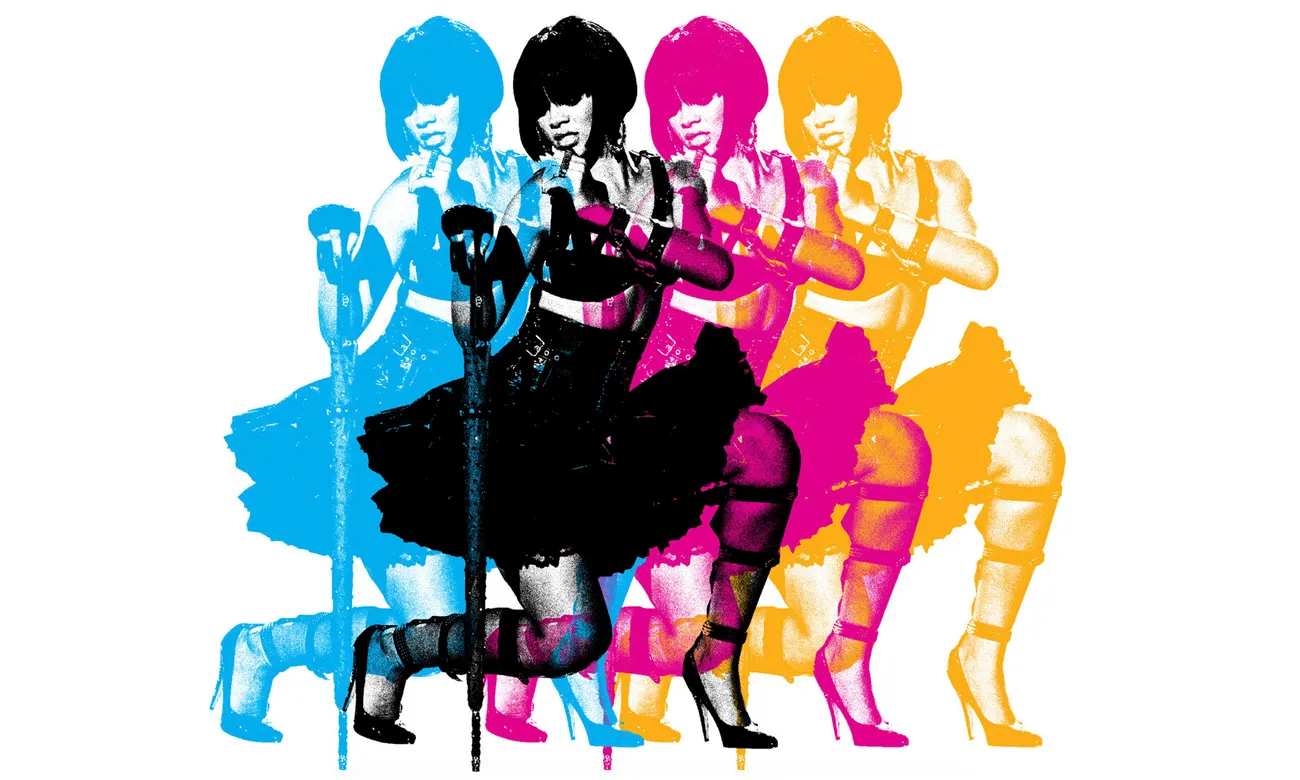
\includegraphics[width=1\textwidth]{misc/title.png}
  \label{titelbild}
\end{figure}

\begin{center}
\textbf{}


\end{center} 

\vspace{1.0cm}


\end{titlepage}
%\restoregeometry

\ifdefined\Shaded\renewenvironment{Shaded}{\begin{tcolorbox}[breakable, frame hidden, interior hidden, enhanced, boxrule=0pt, sharp corners, borderline west={3pt}{0pt}{shadecolor}]}{\end{tcolorbox}}\fi

\renewcommand*\contentsname{Table of contents}
{
\setcounter{tocdepth}{2}
\tableofcontents
}
\mainmatter
\bookmarksetup{startatroot}

\hypertarget{title}{%
\chapter*{Welcome}\label{title}}
\addcontentsline{toc}{chapter}{Welcome}

\markboth{Welcome}{Welcome}

A collection of hand picked songs. This book is hosted as an online
version on \url{http://songs.ratnaweera.net/} and includes a pdf version
(click on the download symbol). Edits and feedback can be made via the
\href{https://github.com/ratnanil/songs}{github repo}.

\part{Selected Songs}

\hypertarget{i-will-follow-you-into-the-dark}{%
\chapter{I will follow you into the
Dark}\label{i-will-follow-you-into-the-dark}}

{[}C{]}\\
Love of mine\\
\hspace*{0.333em} ~ ~ ~ ~ ~ ~ ~{[}Am{]} (D root note)\\
Someday you will die\\
\hspace*{0.333em} ~ ~ ~ ~ ~ ~ ~ ~ ~ {[}F{]}\\
But I will be close behind\\
\hspace*{0.333em} ~ ~ ~ ~{[}C{]} ~ ~ ~ ~ ~ ~ ~ ~{[}G{]}\\
I will follow, you into the dark

No blinding light\\
Or tunnels to gates of white\\
Just our hands clasped so tight\\
Waiting for, the hint of a spark

~{[}Am{]} ~ ~ ~ ~ ~ ~ ~ {[}C{]} ~ ~\\
If heaven and hell decide, ~ ~ ~\\
\hspace*{0.333em} ~ ~ ~ ~{[}F{]} ~ ~ ~ ~ {[}C{]}G\\
that they both are satisfied\\
{[}Am{]} ~ ~ ~ ~ ~ ~{[}C{]} ~ ~ ~ ~ ~ ~ ~ ~G(bar)\\
Illuminate the "no\textquotesingle s", on their vacancy signs\\
{[}Am{]} ~ ~ ~ ~ ~ ~ ~ ~ ~ ~ {[}C{]}\\
If there\textquotesingle s no one beside you,\\
\hspace*{0.333em} ~ ~ ~ ~{[}E{]} ~ ~{[}Am{]}G\\
when your soul embarks\\
Bb ~ ~ ~ ~ ~ ~ ~ ~ Bbm ~ ~ ~ ~ ~ \href{C\%20root\%20note}{F}\\
Then I will follow you into the dark

Catholic school\\
As vicious as roman rule\\
I got my knuckles bruised\\
By a lady in black\\
\hspace*{0.333em} ~\\
And I held my tongue\\
as she told me "son, fear is the heart of love."\\
So I never went back

\{chorus\}

You and me, have seen everything to see\\
From Bangkok to Calgary ~\\
And the soles of your shoes

Are all worn down, the time for sleep is now\\
But it\textquotesingle s nothing to cry about ~\\
Because we\textquotesingle ll hold each other soon\\
{[}Am{]} ~ ~ ~ ~ ~ ~ ~ ~ Fm ~ ~Fm\\
in the blackest of rooms

{[}Am{]} ~ ~ ~ ~ ~ ~ ~ ~{[}C{]} ~ ~\\
If heaven and hell decide,\\
\hspace*{0.333em} ~ ~ ~ ~{[}F{]} ~ ~ ~ ~ ~{[}C{]}G\\
that they both are satisfied\\
{[}Am{]} ~ ~ ~ ~ ~ ~{[}C{]} ~ ~ ~ ~ ~ ~ ~ ~G(bar)\\
Illuminate the "no\textquotesingle s", on their vacancy signs\\
{[}Am{]} ~ ~ ~ ~ ~ ~ ~ ~ ~ ~ {[}C{]} ~ ~ ~ ~ ~ ~{[}E{]} ~ ~{[}Am{]}G\\
If there\textquotesingle s no one beside you, when your soul embarks\\
{[}F{]} ~ ~ ~ ~ ~ ~ ~ Fm ~ ~ ~ ~ ~ {[}C{]} ~\\
Then I will follow you into the dark

E-\/-\/-\/-\/-\/-\/-\/-\/-\/-\/-\/-\/-\/-\/-\/-\/-\/-\/-\/-\/-\textbar{}\\
B-\/-\/-1-\/-\/-1-\/-\/-\/-\/-\/-\/-\/-1-\/-\/-\/-\textbar{}\\
G-\/-\/-2-\/-\/-2-\/-\/-\/-\/-\/-\/-\/-2-\/-\/-\/-\textbar{}\\
D-\/-\/-0-\/-\/-0-\/-\/-\/-\/-\/-\/-\/-2-\/-\/-\/-\textbar{}\\
A-\/-\/-3-\/-\/-2-\/-\/-\/-0-\/-\/-0-\/-\/-\/-\textbar{}\\
E-\/-\/-\/-\/-\/-\/-\/-\/-\/-\/-\/-\/-\/-\/-\/-\/-\/-\/-\/-\/-\textbar{}

{[}F{]} ~ ~ ~ ~ ~ ~ ~ Fm ~ ~ ~ ~ ~ {[}C{]} ~\\
Then I will follow you into the dark

\hypertarget{suzanne}{%
\chapter{Suzanne}\label{suzanne}}

{[}E{]} ~ ~ ~ ~ ~ ~ ~\\
Suzanne takes you down\\
to her place by the river\\
\hspace*{0.333em} ~ ~ ~{[}F\#m{]} ~ ~ ~ ~ ~\\
You can hear the boats go by,\\
you can spend the night beside herw\\
\hspace*{0.333em} ~ ~ ~ {[}E{]} ~ ~ ~ ~ ~ ~ ~ ~ ~\\
And you know that she\textquotesingle s half crazy\\
but that\textquotesingle s why you want to be there\\
\hspace*{0.333em} ~ ~ ~ G\#m ~ ~ ~ ~ ~ ~\\
And she feeds you tea and oranges\\
\hspace*{0.333em} ~ ~ ~ ~{[}A{]} ~ ~ ~ ~ ~ ~ ~\\
that come all the way from China\\
\hspace*{0.333em} ~ {[}E{]}\\
And just when you mean to tell\\
\hspace*{0.333em} ~ ~ ~ ~ ~{[}F\#m{]}\\
her that you have no love to give her\\
\hspace*{0.333em} ~ ~ ~ {[}E{]}\\
Then she gets you on her wavelength\\
\hspace*{0.333em} ~ ~ ~{[}F\#m{]}\\
And she lets the river answer ~ ~ ~ ~ ~ ~ ~ ~ ~ ~ ~ ~\\
\hspace*{0.333em} ~ ~ ~ ~ ~ {[}E{]}\\
that you\textquotesingle ve always been her lover\\
\hspace*{0.333em} ~ ~ ~ {[}G\#m{]}\\
And you want to travel with her\\
\hspace*{0.333em} ~ ~ ~{[}A{]}\\
And you want to travel blind\\
\hspace*{0.333em} ~ ~ ~ {[}E{]}\\
And you know that she will trust you\\
\hspace*{0.333em} ~ ~ ~ ~ ~{[}F\#m{]} ~ ~ ~\\
For you\textquotesingle ve touched her perfect body ~ ~ ~ ~ ~ ~ ~ ~\\
\hspace*{0.333em} ~ ~ ~ ~{[}E{]}\\
with your mind

And Jesus was a sailor\\
when He walked upon the water\\
And He spent a long time watching\\
from his lonely wooden tower\\
And when He knew for certain\\
only drowning men could see Him\\
He said, "All men will be sailors\\
then until the sea shall free them"\\
But He Himself was broken\\
long before the sky would open\\
Forsaken, almost human,\\
He sank beneath your wisdom like a stone

And you want to travel with him\\
And you want to travel blind\\
And you think maybe you\textquotesingle ll trust him\\
For he\textquotesingle s touched your perfect body\\
with his mind

Suzanne takes your hand,\\
and she leads you to the river ~\\
She is wearing rags and feathers\\
from Salvation Army counters\\
And the sun pours down like honey\\
on our lady of the harbor\\
And she shows you where to look\\
among the garbage and the flowers\\
There are heroes in the seaweed,\\
there are children in the morning ~ ~\\
They are leaning out for love\\
and they will lean that way forever ~\\
while Suzanne holds the mirror

And you want to travel with her\\
And you want to travel blind\\
And you know that you will trust her\\
For she\textquotesingle s touched your perfect body\\
with her mind

\hypertarget{for-the-windows-in-paradise}{%
\chapter{For the Windows in
Paradise}\label{for-the-windows-in-paradise}}

{[}Am{]} ~ ~ ~ ~ Fmaj7 ~ ~{[}C{]} ~ ~ ~ ~ ~ ~ {[}G{]}\\
I have called you children, I have called you son,\\
{[}Am{]} ~ ~ ~ ~Fmaj7 ~ ~ {[}C{]} ~ ~ ~ ~ {[}G{]}\\
What is there to answer when I\textquotesingle m the only one?\\
{[}Am{]} ~ ~ ~ ~Fmaj7 ~ {[}C{]} ~ ~ ~ ~ ~ {[}G{]}\\
Morning comes in paradise, morning comes in light,\\
{[}Am{]} ~ ~Fmaj7 ~ {[}C{]} {[}G{]}\\
Still I must obey, still I must invite.

~ ~ ~ ~ ~{[}Am{]} ~ ~ ~ Fmaj7 ~ ~ ~ {[}C{]} ~{[}G{]}\\
If there\textquotesingle s anything to say, if there\textquotesingle s
anything to do,\\
\hspace*{0.333em} ~ ~ ~ ~{[}Am{]} ~ ~ Fmaj7 ~{[}C{]} ~ ~ ~{[}G{]}\\
If there\textquotesingle s any other way, I\textquotesingle ll do
anything for you.

I was dressed embarrassment.\\
I was dressed in wine.\\
If you had a part of me, will you take you\textquotesingle re time?\\
Even if I come back, even if I die\\
Is there some idea to replace my life?

Like a father to impress;\\
Like a mother\textquotesingle s mourning dress,\\
If you ever make a mess, I\textquotesingle ll do anything for you

I have called you preacher; I have called you son.\\
If you have a father or if you haven\textquotesingle t one,\\
I\textquotesingle ll do anything for you (4x)

I did everything for you (repeat.. about 8x)

\hypertarget{all-the-world-is-green}{%
\chapter{All the World is Green}\label{all-the-world-is-green}}

{[}Bm{]} ~ ~ ~ ~ ~ {[}Em{]} ~{[}A7{]} ~ ~ ~ ~ ~ ~{[}D{]}\\
I fell into the ocean ~and you became my wife\\
{[}G7{]} ~ ~ ~ ~ ~ ~ ~ ~ ~ ~ ~ ~ ~ ~ ~ ~ ~ ~ ~ ~{[}Bm{]}\\
I risked it all against the sea to have a better life\\
\hspace*{0.333em} ~ ~ ~ ~{[}Em{]} ~ ~ ~ ~ ~ ~ {[}A7{]} ~ ~ ~ ~ {[}D{]}\\
Marie you are the wild blue sky, men do foolish things\\
{[}G7{]} ~ ~ ~ ~ ~ ~ ~ ~ ~ ~ ~ ~ ~ ~ ~ ~ ~ ~ ~{[}Bm{]}\\
You turn kings into beggars and beggars into kings

~{[}G{]} ~ ~ ~ ~ ~ ~ ~ ~ ~{[}D{]}\\
Pretend that you owe me nothing ~ ~ ~\\
\hspace*{0.333em} {[}A7{]} ~ ~ ~ ~ ~ ~ {[}D{]}\\
and all the world is green\\
{[}G{]} ~ ~ ~ ~ ~ ~ ~ ~ ~ {[}D{]} ~ ~ ~ ~\\
We can bring back the old days again ~ ~\\
\hspace*{0.333em} ~{[}A7{]} ~ ~ ~ ~ ~ ~ {[}D{]}\\
when all the world is green

The face forgives the mirror\\
The worm forgives the plow\\
The questions begs the answer\\
Can you forgive me somehow?

Maybe when our story\textquotesingle s over\\
We\textquotesingle ll go where it\textquotesingle s always spring\\
The band is playing our song again\\
And all the world is green {[}Play Chorus{]}

The moon is yellow silver\\
On the things that summer brings\\
It\textquotesingle s a love you\textquotesingle d kill for\\
And all the world is green

He\textquotesingle s balancing a diamond\\
On a blade of grass\\
The dew will settle on our graves\\
When all the world is green

\{Comment: Play chorus, solo, repeat last verse\}

\hypertarget{dance-me-to-the-end-of-love}{%
\chapter{Dance me to the end of
Love}\label{dance-me-to-the-end-of-love}}

{[}Am{]} ~ ~ ~ ~ ~ ~ ~ ~ ~ ~ ~ ~ ~{[}Em{]}\\
Dance me to your beauty with a burning violin\\
{[}Am{]} ~ ~ ~ ~ ~ ~ ~ ~ ~ ~ ~ ~ ~ ~ ~ {[}Em{]}\\
Dance me through the panic \textquotesingle til I\textquotesingle m
gathered safely in\\
{[}Am{]} ~ ~ ~ ~ ~ ~ ~ ~ ~ ~ ~ ~ ~ ~{[}Em{]}\\
Lift me like an olive branch and be my homeward dove\\
{[}B7{]} ~ ~ ~ ~ ~ ~ ~ ~{[}Em{]}\\
Dance me to the end of love\\
{[}B7{]} ~ ~ ~ ~ ~ ~ ~ ~{[}Em{]}\\
Dance me to the end of love

Oh let me see your beauty when the witnesses are gone\\
Let me feel you moving like they do in Babylon\\
Show me slowly what I only know the limits of\\
Dance me to the end of love\\
Dance me to the end of love

Dance me to the wedding now, dance me on and on\\
Dance me very tenderly and dance me very long\\
We\textquotesingle re both of us beneath our love, we\textquotesingle re
both of us above\\
Dance me to the end of love\\
Dance me to the end of love

Dance me to your beauty with a burning violin\\
Dance me through the panic till I\textquotesingle m gathered safely in\\
Touch me with your naked hand or touch me with your glove\\
Dance me to the end of love (3x)

\{comment: play intro again\}

\hypertarget{build-me-up-buttercup}{%
\chapter{Build me up Buttercup}\label{build-me-up-buttercup}}

Why do you build me up (build me up) Buttercup, baby\\
Just to let me down (let me down)and mess me around\\
And then worst of all (worst of all) you never call, baby\\
When you say you will (say you will) but I love you still\\
I need you (I need you) more than anyone, darlin\textquotesingle{}\\
You know that I have from the start\\
So build me up (build me up) Buttercup,\\
don\textquotesingle t break my heart

"I\textquotesingle ll be over at ten", you told me time and again\\
But you\textquotesingle re late, I wait around and then (bah-dah-dah)\\
I run to the door, I can\textquotesingle t take any more\\
It\textquotesingle s not you, you let me down again

(Hey, hey, hey!) Baby, baby, try to find\\
(Hey, hey, hey!){[}A{]}little time, and I\textquotesingle ll make you
happy\\
(Hey, hey, hey!) I\textquotesingle ll be home\\
I\textquotesingle ll be beside the phone waiting for you\\
Ooo-oo-ooo, ooo-oo-ooo

\{chorus\}

You were my toy but I could be the boy you adore\\
If you\textquotesingle d just let me know (bah-dah-dah)\\
Although you\textquotesingle re untrue, I\textquotesingle m attracted to
you all the more\\
Why do I need you so

\{bridge\}

\{chorus\}

\hypertarget{hallelujah}{%
\chapter{Hallelujah}\label{hallelujah}}

Well I heard there was a secret chord\\
That David played, and it pleased the Lord\\
But you don\textquotesingle t really care for music, do ya?\\
Well it goes like this\\
The fourth, the fifth\\
The minor fall and the major lift\\
The baffled king composing Hallelujah\\
Hallelujah (4x)

Well Your faith was strong but you needed proof\\
You saw her bathing on the roof\\
Her beauty and the moonlight overthrew you\\
she tied you to her kitchen chair\\
And she broke your throne and she cut your hair\\
And from your lips she drew the Hallelujah\\
Hallelujah (4x)

Well baby I\textquotesingle ve been here before\\
I\textquotesingle ve seen this room and I\textquotesingle ve walked this
floor\\
I used to live alone before I knew ya\\
I\textquotesingle ve seen your flag on the marble arch\\
Love is not a victory march\\
It\textquotesingle s a cold and it\textquotesingle s a broken
Hallelujah\\
Hallelujah (4x)

Well there was a time when you let me know\\
What\textquotesingle s really going on below\\
But now you never show that to me do you?\\
And remember when I moved in you?\\
And the holy dove was moving too\\
And every breath we drew was Hallelujah\\
Hallelujah (4x)

Well maybe there\textquotesingle s a God above\\
But all I\textquotesingle ve ever learned from love\\
Was how to shoot somebody who\textquotesingle d OUT DREW YA\\
And it\textquotesingle s not a cry that you hear at night\\
It\textquotesingle s not somebody who\textquotesingle s seen in the
light\\
It\textquotesingle s a cold and it\textquotesingle s a broken
Hallelujah\\
Hallelujah (repeat... hold...)

\hypertarget{jar-of-hearts}{%
\chapter{Jar of Hearts}\label{jar-of-hearts}}

{[}Bm{]} ~ ~ ~ ~ ~ ~ ~ ~ ~ ~ ~ ~ {[}D{]}\\
I know I can\textquotesingle t take one more step towards you\\
{[}A{]} ~ ~ ~ ~ ~ ~ ~ ~ ~ ~ ~ ~ ~ {[}Em{]}\\
\textquotesingle Cause all thats waiting is regret\\
{[}Bm{]} ~ ~ ~ ~ ~ ~ ~ ~ ~ ~ ~ ~ ~ ~{[}D{]}\\
And don\textquotesingle t you know I\textquotesingle m not your ghost
anymore\\
{[}A{]} ~ ~ ~ ~ ~ ~ ~ ~ ~ ~ ~ ~ ~ {[}G{]}\\
You lost the love I loved the most\\
{[}Em{]} ~ ~ ~ ~ ~ ~ ~{[}D{]} ~ ~{[}A{]}\\
I learned to live half a life\\
{[}Em{]} ~ ~ ~ ~{[}D{]} ~ ~ ~ ~ ~ {[}Asus4{]}{[}A{]}\\
And now you want me one more time

{[}D{]} ~ ~ ~ ~ ~ ~ ~ ~ ~{[}A{]}\\
Who do you think you are?\\
\hspace*{0.333em} ~ ~ ~ ~ ~ ~ ~ ~ ~ ~ {[}Bm{]}\\
Running \textquotesingle round leaving scars\\
\hspace*{0.333em} ~ ~ ~ ~ ~ ~ ~ ~ ~ {[}G{]}\\
Collecting a jar of hearts\\
Gm ~ ~ ~ ~ ~ {[}D{]}\\
Tearing love apart\\
{[}D{]} ~ ~ ~ ~ ~ ~ ~ ~ ~{[}A{]}\\
You\textquotesingle re gonna catch a cold\\
\hspace*{0.333em} ~ ~ ~ ~ ~ ~ ~ ~ ~ ~ ~ {[}Bm{]}\\
From the ice inside your soul\\
\hspace*{0.333em} ~ ~ ~ ~ ~ ~ ~ ~ ~{[}G{]}\\
Don\textquotesingle t come back for me\\
Gm ~ ~ ~ ~ ~ ~ ~ ~ ~ {[}D{]}\\
Who do you think you are?

{[}Bm{]} ~ ~ ~ ~ ~ ~ ~ ~ ~ ~ ~{[}D{]}\\
I hear you\textquotesingle re asking all around\\
{[}A{]} ~ ~ ~ ~ ~ ~ ~ ~ ~ ~ {[}Em{]}\\
If I am anywhere to be found\\
{[}Bm{]} ~ ~ ~ ~ ~ ~ ~ ~ ~{[}D{]}\\
But I have grown too strong\\
{[}A{]} ~ ~ ~ ~ ~ ~ ~ ~ ~ ~ ~ {[}G{]}\\
To ever fall back in your arms\\
{[}Em{]} ~ ~ ~ ~ ~ ~ ~ ~ {[}D{]} ~ ~{[}A{]}\\
I\textquotesingle ve learned to live half a life\\
{[}Em{]} ~ ~ ~ ~{[}D{]} ~ ~ ~ ~ ~{[}Asus4{]}{[}A{]}\\
And now you want me one more time

\{chorus\}

{[}Bm{]} ~ ~ ~ {[}F\#{]} ~ ~ ~ ~ {[}D{]} ~ ~ {[}E{]}\\
It took so long just to feel alright\\
{[}Bm{]} ~ ~ ~ ~ ~{[}F\#{]} ~ ~ ~ ~ ~ {[}D{]} ~ ~ ~ ~{[}E{]}\\
Remember how to put back the light in my eyes\\
\hspace*{0.333em}{[}Bm{]} ~ ~ ~ ~{[}F\#{]} ~ ~ ~ ~ ~ ~{[}D{]} ~ ~ ~ ~ ~
{[}E{]}\\
I wish I had missed the first time that we kissed\\
\hspace*{0.333em} ~ ~ {[}Bm{]} ~ ~ ~{[}F\#{]} ~ ~ {[}D{]} ~ {[}E{]}\\
\textquotesingle Cause you broke all your promises\\
\hspace*{0.333em} ~{[}G{]}\\
And now you\textquotesingle re back\\
\hspace*{0.333em} ~ ~ ~ ~ ~ ~ ~{[}F\#{]}\\
You don\textquotesingle t get to get me back

\{chorus\}

\{comment: (...Don\textquotesingle t come back at all) x2\}

Gm ~ ~ ~ ~ ~ ~ ~ ~ ~ ~{[}D{]}\\
Who do you think you are?\\
Gm ~ ~ ~ ~ ~ ~ ~ ~ ~ ~{[}D{]}\\
Who do you think you are?\\
Gm ~ ~ ~ ~ ~ ~ ~ ~ ~ ~{[}D{]}\\
Who do you think you are?

\hypertarget{new-slang}{%
\chapter{New Slang}\label{new-slang}}

Am C F C G C Am G x4\\
C

{[}Am{]} ~ ~ ~ ~ ~ ~{[}C{]} ~ ~ ~ ~ ~ ~{[}F{]}\\
Gold teeth and a curse for this town\\
{[}C{]} ~ ~ ~ ~ ~ {[}G{]}\\
Were all in my mouth\\
\hspace*{0.333em} ~{[}C{]} ~ ~ ~ ~ ~{[}F{]} ~ ~ ~ ~ ~{[}Am{]} {[}G{]}\\
Only I don\textquotesingle t know how they got out, dear\\
{[}Am{]} ~ ~ ~ ~ ~{[}C{]} ~ ~{[}F{]}\\
Turn me back into the pet\\
{[}C{]} ~ ~ ~ ~ ~{[}G{]}\\
I was when we met\\
{[}C{]} ~ ~ ~ ~ ~{[}F{]} ~ ~ ~ ~ ~{[}Am{]} {[}G{]}\\
I was happier then with no mind set

{[}G{]} ~ ~ ~ ~ ~ ~ ~ ~ ~ {[}C{]}\\
And if you\textquotesingle d a took to me like\\
{[}F{]} ~{[}C{]} ~ ~ ~ ~ ~{[}G{]}\\
A gull takes to the wind\\
\hspace*{0.333em} ~ ~ ~ ~ {[}G{]} ~ ~ ~ ~ {[}C{]}\\
Well, I\textquotesingle d a jumped from my tree\\
\hspace*{0.333em} {[}F{]} ~ {[}C{]} ~ ~ ~ ~ ~ ~ {[}F{]} ~ ~ ~ ~
{[}C{]}\\
And I\textquotesingle d a danced like the king of the eyesores\\
{[}F{]} ~ ~ ~ ~ ~ ~ ~ ~{[}C{]} ~ ~ ~ ~ ~ {[}G{]}\\
And the rest of our lives would\textquotesingle a fared well

{[}Am{]} ~ ~ ~ ~ ~ ~ ~{[}C{]} ~ ~ ~ ~{[}F{]}\\
New slang when you notice the stripes\\
{[}C{]} ~ ~ ~ ~ ~ ~ {[}G{]}\\
The dirt in your fries\\
\hspace*{0.333em} ~{[}C{]} ~ ~ ~ ~ ~ ~ ~ ~ {[}F{]}\\
Hope it\textquotesingle s right when you die\\
\hspace*{0.333em} ~ ~ {[}Am{]}{[}G{]}\\
Old and bo..ny\\
{[}Am{]} ~ ~ ~ ~ ~ ~ ~{[}C{]} ~ ~ ~ ~ ~ ~ ~{[}F{]}\\
Dawn breaks like a bull through the hall\\
{[}C{]} ~ ~ ~ ~ ~ {[}G{]}\\
Never should\textquotesingle a called\\
\hspace*{0.333em} {[}C{]} ~ ~ ~ ~ ~ ~ {[}F{]}\\
But my heads to the wall\\
\hspace*{0.333em} ~ ~ {[}Am{]}{[}G{]}\\
And I\textquotesingle m lonely

\{chorus\}

{[}Am{]} ~ ~ ~ ~ ~ ~ {[}C{]} ~ ~ ~ ~{[}F{]}\\
God speed all the baker\textquotesingle s at dawn\\
\hspace*{0.333em} ~ ~ ~ ~ ~{[}C{]} ~ ~ ~ {[}G{]}\\
May they all cut their thumbs\\
\hspace*{0.333em} {[}C{]} ~ ~ ~ ~ ~ ~ ~{[}F{]}\\
And bleed into their buns\\
\hspace*{0.333em} ~ ~ ~ ~{[}Am{]} {[}G{]}\\
\textquotesingle Till they melt away

\{start.of.chorus: Chorus 2\}\\
{[}G{]} ~ ~ ~ ~ ~ ~ ~ ~ ~ {[}C{]}\\
I\textquotesingle m looking in on the good life\\
\hspace*{0.333em} ~ ~ ~ ~{[}F{]} ~ ~{[}C{]} ~ ~ ~{[}G{]}\\
I might be doomed never to find\\
\hspace*{0.333em} ~ ~ ~ ~ ~ ~ ~ ~ ~ ~ ~ ~{[}C{]}\\
Without a trust or flaming fields\\
\hspace*{0.333em} ~{[}F{]} {[}C{]} ~ ~ {[}G{]}\\
{[}Am{]} too dumb to refine?\\
\hspace*{0.333em} ~ ~ ~ ~ ~ ~ ~ ~ ~ ~{[}C{]}\\
And if you\textquotesingle d a took to me like\\
\hspace*{0.333em} ~{[}F{]} ~ {[}C{]} ~ ~ ~ ~ ~ ~ {[}F{]} ~ ~ ~ ~
~{[}C{]}\\
Well I\textquotesingle d a danced like the queen of the eyesores\\
{[}F{]} ~ ~ ~ ~ ~ ~ ~ ~{[}C{]} ~ ~ ~ ~ ~ {[}G{]}\\
And the rest of our lives would\textquotesingle a fared well\\
:::

\hypertarget{viva-la-vida}{%
\chapter{Viva la Vida}\label{viva-la-vida}}

C - D - G - Em

(Em) ~ ~ {[}C{]} ~ ~ ~{[}D{]}\\
I used to rule the world\\
\hspace*{0.333em} ~ ~ ~ ~{[}G{]} ~ ~ ~ ~ ~ ~ ~ ~ ~{[}Em{]}\\
Seas would rise when I gave the word\\
\hspace*{0.333em} ~ ~ ~ ~ ~ ~ ~ ~ ~{[}C{]} ~ ~ {[}D{]}\\
Now in the morning I sleep alone\\
\hspace*{0.333em} ~ ~ ~ {[}G{]} ~ ~ ~ ~ ~ ~ ~ {[}Em{]}\\
Sweep the streets I used to own

C - D - G - Em ~ ~x2

I used to roll the dice\\
Feel the fear in my enemy\textquotesingle s eyes\\
Listen as the crowd would sing\\
"Now the old king is dead! Long live the king!"

One minute I held the key\\
Next the walls were closed on me\\
And I discovered that my castles stand\\
Upon pillars of salt and pillars of sand

{[}C{]} ~ ~ ~ ~ ~ ~{[}D{]}\\
I hear Jerusalem bells are ringing\\
{[}G{]} ~ ~ ~ ~ ~{[}Em{]}\\
Roman Cavalry choirs are singing\\
{[}C{]} ~ ~ ~ ~ ~ ~ {[}D{]}\\
Be my mirror, my sword, and shield\\
\hspace*{0.333em}{[}G{]} ~ ~ ~ ~ ~ ~ ~ {[}Em{]}\\
My missionaries in a foreign field\\
{[}C{]} ~ ~ ~ ~ ~ ~ ~{[}D{]}\\
For some reason I can\textquotesingle t explain\\
{[}G{]} ~ ~ ~ ~ ~ ~ ~ ~ ~{[}Em{]} ~ ~ ~ ~ ~ ~{[}C{]} ~ ~{[}D{]}\\
Once you go there was never, never an honest word\\
\hspace*{0.333em} ~ ~ ~{[}Bm{]} ~ ~ ~ ~ ~ ~ {[}Em{]}\\
That was when I ruled the world

It was the wicked and wild wind\\
Blew down the doors to let me in\\
Shattered windows and the sound of drums\\
People couldn\textquotesingle t believe what I\textquotesingle d become

Revolutionaries wait\\
For my head on a silver plate\\
Just a puppet on a lonely string\\
Oh who would ever want to be king?

\{chorus\}

\hypertarget{wagon-wheel}{%
\chapter{Wagon Wheel}\label{wagon-wheel}}

{[}G{]} ~ ~ ~ ~ ~ ~ ~ ~ ~ ~ {[}D{]}\\
Headed down south to the land of the pines\\
\hspace*{0.333em} ~ ~ {[}Em{]} ~ ~ ~ ~ ~ ~ ~ ~ {[}C{]}\\
And I\textquotesingle m thumbin\textquotesingle{} my way into North
Caroline\\
{[}G{]}\\
Starin\textquotesingle{} up the road\\
\hspace*{0.333em} ~ ~ ~ ~ {[}D{]} ~ ~ ~ {[}C{]}\\
And pray to God I see headlights

I made it down the coast in seventeen hours\\
Pickin\textquotesingle{} me a bouquet of dogwood flowers\\
And I\textquotesingle m a hopin\textquotesingle{} for Raleigh\\
I can see my baby tonight

~{[}G{]} ~ ~ ~ ~ ~ ~ ~ ~ {[}D{]}\\
So rock me mama like a wagon wheel\\
{[}Em{]} ~ ~ ~ ~ ~ {[}C{]}\\
Rock me mama anyway you feel\\
{[}G{]}{[}D{]} ~ {[}C{]}\\
Hey, mama rock me\\
{[}G{]} ~ ~ ~ ~ ~ ~ ~ ~ ~{[}D{]}\\
Rock me mama like the wind and the rain\\
{[}Em{]} ~ ~ ~ ~ ~ ~ ~ {[}C{]}\\
Rock me mama like a south-bound train\\
{[}G{]}{[}D{]} ~ {[}C{]}\\
Hey, mama rock me

Intro

Runnin\textquotesingle{} from the cold up in New England\\
I was born to be a fiddler in an old-time stringband\\
My baby plays the guitar\\
I pick a banjo now

Oh, the North country winters keep a gettin\textquotesingle{} me now\\
Lost my money playin\textquotesingle{} poker so I had to up and leave\\
But I ain\textquotesingle t a turnin\textquotesingle{} back\\
To livin\textquotesingle{} that old life no more

\{chorus\}

Walkin\textquotesingle{} to the south out of Roanoke\\
I caught a trucker out of Philly\\
Had a nice long toke\\
But he\textquotesingle s a headed west from the Cumberland Gap\\
To Johnson City, Tennessee

And I gotta get a move on before the sun\\
I hear my baby callin\textquotesingle{} my name\\
And I know that she\textquotesingle s the only one\\
And if I die in Raleigh\\
At least I will die free

\{chorus\}

\hypertarget{mad-world}{%
\chapter{Mad World}\label{mad-world}}

All around me are familiar faces\\
Worn out places, worn out faces\\
Bright and early for their daily races\\
Going nowhere, going nowhere\\
Their tears are filling up their glasses\\
No expression, no expression\\
Hide my head, I want to drown my sorrow\\
No tomorrow, no tomorrow

And I find it kinda funny, I find it kinda sad\\
The dreams in which I\textquotesingle m dying are the best
I\textquotesingle ve ever had\\
I find it hard to tell you, I find it hard to take\\
When people run in circles it\textquotesingle s a very very\\
Mad world, mad world

Children waiting for the day, they feel good\\
Happy birthday, happy birthday\\
Made to feel the way that every child should\\
Sit and listen, sit and listen

Went to school and I was very nervous\\
No one knew me, no one knew me\\
Hello teacher, tell me what\textquotesingle s my lesson\\
Look right through me, look right through me

And I find it kinda funny, I find it kinda sad\\
The dreams in which I\textquotesingle m dying are the best
I\textquotesingle ve ever had\\
I find it hard to tell you, I find it hard to take\\
When people run in circles it\textquotesingle s a very very\\
Mad world, mad world\\
Enlarge your world\\
Mad world

\part{Guitar Classics}

\hypertarget{hurt}{%
\chapter{Hurt}\label{hurt}}

{[}Am{]}{[}C{]} ~ ~ {[}D{]} ~ {[}Am{]} ~ ~ {[}C{]} ~ ~{[}D{]} ~ ~
{[}Am{]}\\
\hspace*{0.333em} I hurt myself today ~ to see if I still feel\\
{[}C{]} ~{[}D{]} ~ ~ ~{[}Am{]} ~ ~ ~{[}C{]} ~ ~{[}D{]} ~ ~ ~ ~{[}Am{]}\\
I focus on the pain ~ the only thing that\textquotesingle s real\\
\hspace*{0.333em} {[}C{]} ~ ~{[}D{]} ~ ~ {[}Am{]} ~ ~ ~ {[}C{]} ~
~{[}D{]} ~ ~ {[}Am{]}\\
The needle tears a hole ~ the old familiar sting\\
\hspace*{0.333em} ~ ~{[}C{]} ~ ~{[}D{]} ~ ~{[}Am{]} ~ ~ ~ ~ {[}C{]} ~
~{[}D{]} ~ ~{[}G{]} ~ ~ ~ ~\\
Try to kill it all away ~ but I remember everything

{[}Am{]} ~ ~ ~ ~ ~ {[}F{]} ~ {[}C{]} ~ ~ ~ ~ ~ ~ {[}G{]}\\
What have I become? ~ ~ My sweetest friend\\
{[}Am{]} ~ ~ ~ {[}F{]} ~ ~ ~ ~ ~ {[}C{]} ~ ~ ~{[}G{]}\\
Everyone I know ~goes away in the end\\
\hspace*{0.333em} {[}Am{]} ~ ~ ~ ~ ~ ~ ~ {[}F{]} ~{[}G{]} ~ ~ ~ ~ ~ ~
{[}G{]}\\
And you could have it all ~ My empire of dirt\\
{[}Am{]} ~ ~ ~ ~ ~ {[}F{]} ~ ~{[}G{]} ~ ~ ~ ~ ~ ~ ~{[}Am{]}\\
I will let you down ~ ~I will make you hurt

I wear this crown of thorns ~ upon my liar\textquotesingle s chair\\
Full of broken thoughts ~ I cannot repair\\
Beneath the stains of time ~ the feelings disappear\\
You are someone else ~ I am still right here

\{chorus\}

~{[}Am{]} ~ ~ ~ ~ ~ ~ {[}F{]} ~ {[}G{]} ~ ~ ~ ~ ~ ~{[}G{]}\\
If I could start again ~a million miles away\\
{[}Am{]} ~ ~ ~ ~ ~ {[}F{]} ~{[}G{]}\\
I would keep myself ~I would find a way

\hypertarget{where-have-all-the-flowers-gone}{%
\chapter{Where have all the flowers
Gone?}\label{where-have-all-the-flowers-gone}}

C ~ ~ ~ ~ ~ ~ ~ ~ ~Am ~ ~ ~ ~ ~ ~F ~ ~ ~ ~ ~G\\
Where have all the flowers gone, long time passing\\
C ~ ~ ~ ~ ~ ~ ~ ~ ~Am ~ ~ ~ ~ ~ ~F ~ ~ ~ ~ ~G\\
Where have all the flowers gone, long time ago\\
C ~ ~ ~ ~ ~ ~ ~ ~ ~Am ~ ~ ~ ~ ~ ~F ~ ~ ~ ~ ~ G\\
Where have all the flowers gone, young girls picked them every one\\
F ~ ~ ~ ~ C ~ ~ ~ ~ ~ ~ ~ ~ ~F ~ ~ ~ ~ G ~ ~ ~ ~ ~C ~\\
When will they ever learn? , when will they ever learn?

C ~ ~ ~ ~ ~ ~ ~ ~ ~ Am ~ ~ ~ ~ ~ F ~ ~ ~ ~ ~ ~G\\
Where have all the young girls gone, Gone to young men every one

C ~ ~ ~ ~ ~ ~ ~ ~ ~ Am ~ ~ ~ ~ ~ F ~ ~ ~ ~ ~ ~G\\
Where have all the young men gone, Gone to soldiers every one

C ~ ~ ~ ~ ~ ~ ~ ~ ~ Am ~ ~ ~ ~ ~ F ~ ~ ~ ~ ~ ~G ~\\
Where have all the soldiers gone, Gone to graves every one

C ~ ~ ~ ~ ~ ~ ~ ~ ~ Am ~ ~ ~ ~ ~ F ~ ~ ~ ~ ~ ~G ~\\
Where have all the graves gone, Gone to flowers every one.

F ~ ~ ~ ~ C ~ ~ ~ ~ ~ ~ ~ ~ ~F ~ ~ ~ ~ G ~ ~ ~ ~ ~C\\
When will they ever learn? , when will they ever learn?

\hypertarget{ein-bett-im-kornfeld}{%
\chapter{Ein Bett im Kornfeld}\label{ein-bett-im-kornfeld}}

{[}D{]}\\
Sommerabend über blühendem Land.\\
Schon seit Mittag stand ich am\\
Straßenrand.\\
\hspace*{0.333em} ~ ~ ~ ~ {[}A{]}\\
Bei jedem Wagen, der vorüber fuhr,\\
\hspace*{0.333em} ~ ~ ~ ~ ~{[}D{]}\\
hob ich den Daumen.\\
auf einem Fahrrad kam da ein\\
Mädchen her.\\
Und sie sagte: "Ich bedaure dich sehr."\\
\hspace*{0.333em} ~ ~ ~ ~{[}A{]} ~ ~ ~ ~ ~ ~ ~ ~ ~ ~ ~ ~ ~ ~ ~ ~ ~ ~ ~ ~
{[}D{]}\\
Doch ich lachte und sprach: "Ich brauch keine weichen Daunen"

~ ~ ~ ~ ~ ~ {[}G{]}\\
Ein Bett im Kornfeld,\\
Das ist immer frei, denn es ist\\
{[}D{]}\\
Sommer, und was ist schon dabei.\\
\hspace*{0.333em} ~ ~ ~ ~ ~{[}A{]}\\
Die Grillen singen und es duftet\\
\hspace*{0.333em} ~ ~ ~ ~ ~ ~ ~ ~ {[}D{]}\\
nach Heu, wenn ich träume.\\
\hspace*{0.333em} ~ ~ ~ ~ ~ {[}G{]}\\
Ein Bett im Kornfeld, zwischen\\
Blumen und Stroh,\\
\hspace*{0.333em} ~ ~ ~ {[}D{]}\\
Und die Sterne leuchten mir sowieso\\
\hspace*{0.333em} ~ ~ ~ ~ ~ {[}A{]}\\
Ein Bett im Kornfeld mach ich mir\\
\hspace*{0.333em} ~ ~ ~ ~ ~ ~ {[}D{]}\\
irgendwo ganz alleine.

{[}D{]}\\
Etwas später lag ihr Fahrrad im\\
Gras, Und so kam es, dass sie die\\
Zeit vergass,\\
\hspace*{0.333em} ~ ~ ~ {[}A{]}\\
Mit der Gitarre hab ich ihr erzählt\\
\hspace*{0.333em} ~ ~ ~ ~ {[}D{]}\\
Von meinem Leben.\\
Auf einmal rief sie\\
"Es ist höchste Zeit, Schon ist es\\
dunkel und mein Weg ist noch Weit"\\
\hspace*{0.333em} ~ ~ ~ ~{[}A{]}\\
Doch ich lachte und sprach:\\
\hspace*{0.333em} ~ ~ ~ ~ ~ ~ ~ ~ ~ ~ ~ ~ {[}D{]}\\
"Ich hab dir noch viel zu geben".

\{chorus\}

\hypertarget{house-of-the-rising-sun}{%
\chapter{House of the Rising Sun}\label{house-of-the-rising-sun}}

:::\{.song-grid\} \\
Am, C, D, F, Am, E, Am , E\\
:::

~ ~ {[}Am{]} {[}C{]} ~ ~ ~{[}D{]} ~ ~ ~ ~ {[}F{]}\\
There is a house in New Orleans\\
\hspace*{0.333em} ~{[}Am{]} ~ ~ {[}C{]} ~ ~{[}E{]} ~{[}E7{]}\\
They call the Risin\textquotesingle{} Sun\\
\hspace*{0.333em} ~ ~ ~{[}Am{]} ~ ~ {[}C{]} ~ ~ {[}D{]} ~ ~ ~ ~
{[}F{]}\\
And it\textquotesingle s been the ruin of many a poor boy.\\
\hspace*{0.333em} {[}Am{]} ~ {[}E{]} ~ ~ ~{[}Am{]}\\
And God, I know I\textquotesingle m one.

My mother was a tailor.\\
She sewed my new blue jeans.\\
My father was a gamblin\textquotesingle{} man\\
Down in New Orleans.

C, D, F, Am, E, Am , E

Now, the only thing a gambler needs\\
Is a suitcase and a trunk\\
And the only time that he\textquotesingle s satisfied\\
Is when he\textquotesingle s on a drunk

Oh, Mothers, tell your children\\
Not to do what I have done.\\
Spend your lives in sin and misery\\
In the house of the risin\textquotesingle{} sun.

Well, I\textquotesingle ve got one foot on the platform.\\
the other foot on the train.\\
I\textquotesingle m goin\textquotesingle{} down to New Orleans\\
To wear that ball and chain.

\{comment: Play first verse again\}

\hypertarget{sweet-home-alabama}{%
\chapter{Sweet Home Alabama}\label{sweet-home-alabama}}

e\textbar-\/-\/-\/-\/-\/-\/-\/-\/-\/-\/-\/-\/-\/-\/-\/-\/-\/-\/-\/-\/-\/-\/-\/-\/-3-\textbar{}\\
B\textbar-\/-\/-\/-\/-3-\/-\/-\/-\/-\/-\/-\/-\/-3-\/-\/-\/-\/-\/-\/-\/-\/-3-\textbar{}\\
G\textbar-\/-\/-\/-\/-\/-\/-2-\/-\/-\/-\/-\/-\/-\/-\/-\/-0-\/-\/-\/-\/-\/-0-\textbar{}
~x4\\
D\textbar-0-0-\/-\/-\/-\/-\/-\/-\/-\/-\/-\/-\/-\/-\/-\/-\/-\/-\/-\/-\/-\/-0-\textbar{}
~ ~\\
A\textbar-\/-\/-\/-\/-\/-\/-\/-\/-\/-3-3-\/-\/-\/-\/-\/-\/-\/-\/-\/-\/-\/-2-\textbar{}\\
E\textbar-\/-\/-\/-\/-\/-\/-\/-\/-\/-\/-\/-\/-\/-\/-\/-\/-\/-\/-\/-\/-3-3-3-\textbar{}

{[}D{]} {[}Cadd9{]} ~ ~ ~ {[}G{]}\\
Big wheels keep on turning\\
{[}D{]} ~ ~ {[}Cadd9{]} ~ ~ ~ ~{[}G{]}\\
Carry me home to see my kin\\
{[}D{]} ~ ~{[}Cadd9{]} ~ ~ ~ ~ {[}G{]}\\
Singing songs about the south land\\
{[}D{]} ~ ~ {[}Cadd9{]} ~ ~ ~ ~{[}G{]} ~ ~ ~ ~ ~ ~ ~ ~ ~ ~ ~ ~ ~\\
I miss \textquotesingle ole\textquotesingle{} \textquotesingle bamy once
again and I think it\textquotesingle s a sin

{[}D{]} ~ ~ ~ ~ ~ ~ {[}Cadd9{]} ~ ~ ~ ~ ~{[}G{]}\\
Well I heard Mr. Young sing about her\\
{[}D{]} ~ ~ ~ ~ ~ ~ {[}Cadd9{]} ~ ~ ~{[}G{]}\\
Well I heard old Neil put her down\\
{[}D{]} ~ ~ ~ ~ ~ ~ {[}Cadd9{]} ~ ~{[}G{]}\\
Well I hope Neil Young will remember\\
{[}D{]} ~ ~ ~ {[}Cadd9{]} ~ ~ ~ ~ ~ ~{[}G{]} ~ ~ ~ ~ ~ ~ ~\\
{[}A{]}outhern man don't need him around, anyhow

{[}Chorus{]}

{[}D{]} ~{[}Cadd9{]} {[}G{]} ~ {[}D{]} ~ ~ ~ {[}Cadd9{]} ~ ~ ~{[}G{]} ~
~ ~ ~\\
Sweet home Alabama, where the skies are so blue\\
{[}D{]} ~{[}Cadd9{]} {[}G{]} ~ {[}D{]} ~ ~ ~ {[}Cadd9{]} ~ ~ ~ {[}G{]} ~
~\\
Sweet home Alabama, lord I'm coming home to you.

{[}F{]}\\
{[}D{]}add9{[}G{]}\\
{[}D{]}add9{[}G{]}

{[}D{]} ~ ~ ~{[}Cadd9{]} ~ ~ ~ ~ ~ {[}G{]} ~ ~ ~{[}F{]} {[}C{]}
{[}D{]}\\
In Birmingham they love the Gov\textquotesingle nor, boo-hoo-hoo\\
{[}D{]} ~ ~ ~ {[}Cadd9{]} ~ ~ ~ ~ ~ {[}G{]}\\
Now we all did what we could do\\
{[}D{]} ~ ~ ~{[}Cadd9{]} ~ ~ {[}G{]}\\
Now watergate doesn\textquotesingle t bother me\\
{[}D{]} ~ ~ ~{[}Cadd9{]} ~ ~ ~ ~ ~{[}G{]}\\
Does you conscience bother you, (now tell the truth!)

\{chorus\}

{[}D{]}{[}Cadd9{]} ~ ~ ~ ~ ~ ~ ~ ~ ~ {[}G{]}\\
Now Muscle Shoals has got the Swappers\\
{[}D{]} ~ ~ ~ ~ ~ ~ {[}Cadd9{]} ~ ~ ~ ~ ~ ~ ~ ~ {[}G{]}\\
And they\textquotesingle ve been known to pick a song or two (yes we
do)\\
{[}D{]} ~ ~ ~{[}Cadd9{]} ~ ~ ~ {[}G{]}\\
Lord they get me off so much\\
{[}D{]} ~ ~ ~ ~ {[}Cadd9{]} ~ ~ ~ ~ ~ ~{[}G{]} ~\\
They pick me up when I\textquotesingle m feeling blue, Now how about
you?

\{chorus\}

{[}D{]} ~{[}Cadd9{]} {[}G{]} ~ ~\\
Sweet home Alabama (Oh sweet home baby)\\
{[}D{]} ~ ~ ~{[}Cadd9{]} ~ ~ ~{[}G{]} ~\\
Where the skies are so blue (And the governor\textquotesingle s true)\\
{[}D{]} ~{[}Cadd9{]} {[}G{]}\\
Sweet Home Alabama, (Lord, yeah)\\
{[}D{]} ~ ~ ~{[}Cadd9{]} ~ ~ ~ ~{[}G{]}\\
Lord, I\textquotesingle m coming home to you

\hypertarget{streets-of-london}{%
\chapter{Streets of London}\label{streets-of-london}}

{[}C{]} ~ ~ ~ ~ ~ ~ ~{[}G{]} ~ ~ ~{[}Am{]} ~ ~ ~ ~ ~ ~ ~ {[}Em{]}\\
Have you seen the old man, in the closed-down market\\
{[}F{]} ~ ~ ~ ~ ~ {[}C{]} ~ ~ ~ ~ ~ ~ ~{[}D7{]} ~ ~ {[}G7{]}\\
picking up the papers, with his worn-out shoes?\\
{[}C{]} ~ ~ ~ ~ ~ ~{[}G{]} ~ ~ ~ ~ ~ {[}Am{]} ~ ~ ~ ~ ~ ~ {[}Em{]}\\
In his eyes you see no pride, and held loosely by his side\\
{[}F{]} ~ ~ ~ ~{[}C{]} ~ ~ ~ ~ ~ ~ {[}G7{]} ~ ~ ~ ~{[}C{]}\\
yesterday\textquotesingle s papers, telling yesterday\textquotesingle s
news

~ ~ {[}F{]} ~ ~ ~ ~ {[}Em{]} ~ ~ ~ ~ ~ ~{[}C{]} ~{[}G7{]} ~ {[}Am{]}\\
\hspace*{0.333em} ~So how can you tell me, you\textquotesingle re lo -
ne - ly\\
{[}D7{]} ~ ~ ~ ~ {[}D7{]} ~ ~ ~ ~ ~ ~ ~ ~ ~ {[}G{]} ~ ~{[}G7{]}\\
\hspace*{0.333em}and say for you that the sun don\textquotesingle t
shine?\\
{[}C{]} ~ ~ ~ ~ ~ ~{[}G{]} ~ ~ ~ ~ ~ ~ ~{[}Am{]} ~ ~ ~ ~ ~ ~ ~ ~
{[}Em{]}\\
Let me take you by the hand, and lead you through the streets of
London\\
{[}F{]} ~ ~ ~ ~ ~ ~{[}C{]} ~ ~ ~ ~ ~ {[}G7{]} ~ ~ ~ ~ ~ ~ ~ ~ {[}C{]} ~
~{[}C{]}\\
\hspace*{0.333em}I\textquotesingle ll show you something, to make you
change your mind

Have you seen the old gal, who walks the streets of London\\
dirt in her hair, and her clothes in rags?\\
She\textquotesingle s no time for talking, she just keeps right on
walking\\
Carrying her home, in two carrier bags

\{chorus\}

And in the all-night cafe, at a quarter past eleven\\
some old man sitting there, all on his own\\
Looking at the world, over the rim of his tea-cup\\
Each day lasts an hour, then he wanders home alone

\{chorus\}

And have you seen the old man, outside the seaman\textquotesingle s
mission?\\
His memory\textquotesingle s fading, with those medal ribbons that he
wears\\
And in our winter city, the rain cries little pity\\
For one more forgotten hero, and a world that doesn\textquotesingle t
care

\hypertarget{california-dreaming}{%
\chapter{California Dreaming}\label{california-dreaming}}

~ ~NC/(Em) ~ ~ ~ ~ ~{[}Am{]} ~ ~ ~{[}G{]} ~ ~ ~ ~{[}F{]}\\
All the leaves are brown (all the leaves are brown)\\
\hspace*{0.333em} ~ ~ {[}G{]} ~ ~{[}Am{]} ~ ~ ~ ~ ~ ~ ~ ~ ~ {[}E{]}\\
And the sky is gray ~(and the sky is gray)\\
\hspace*{0.333em} ~ ~{[}F{]} ~ ~ ~ ~ ~ ~ {[}C{]} ~ ~ ~ ~{[}E{]}
~{[}Am{]}\\
I\textquotesingle ve been for a walk ~(I\textquotesingle ve been for a
walk)\\
\hspace*{0.333em} ~ {[}F{]} ~ ~ ~{[}Am{]} ~ ~ ~ ~ ~ ~ ~ ~{[}E{]}\\
On a winter\textquotesingle s day ~(on a winter\textquotesingle s day)\\
\hspace*{0.333em} ~ ~ {[}E{]} ~ ~ ~ ~ ~ ~ {[}Am{]} ~ ~{[}G{]} ~ ~
~{[}F{]}\\
I\textquotesingle d be safe and warm (I\textquotesingle d be safe and
warm)\\
\hspace*{0.333em} ~{[}G{]} ~ ~{[}Am{]} ~ ~ ~ ~ ~ ~ ~ {[}E{]}\\
If I was in L.A. ~(if I was in L.A.)

{[}E{]} ~ ~ ~ ~ ~{[}Am{]} ~ ~ {[}G{]} ~ ~ ~ {[}F{]}\\
California dreamin ~(California dreamin\textquotesingle)\\
\hspace*{0.333em} {[}G{]} ~ ~{[}Am{]} ~ ~ {[}E{]}\\
On such a winter\textquotesingle s day

{[}E{]} ~ ~ ~ ~ ~ ~{[}Am{]}\\
Stopped in to a church\\
{[}G{]} ~ ~ ~ ~ ~{[}F{]}\\
I passed along the way\\
\hspace*{0.333em} ~ ~ {[}G{]} ~ ~ ~ ~ ~ ~{[}Am{]} ~ ~ ~ ~ ~ ~{[}E{]}\\
Well I got down on my knees (got down on my knees)\\
{[}F{]} ~ ~ ~ ~ ~ ~ {[}Am{]} ~ ~ ~ ~ ~ ~ ~ {[}E{]}\\
And I pretend to pray (I pretend to pray)\\
{[}E{]} ~ ~ ~ ~ ~ ~ ~ ~ ~{[}Am{]} ~ ~ ~{[}G{]} ~ ~ ~ ~ ~ ~ ~ ~{[}F{]}\\
You know the preacher likes the cold (preacher likes the cold)\\
\hspace*{0.333em} ~ ~ ~{[}G{]} ~ ~ ~ {[}Am{]} ~ ~ ~ ~ ~ ~ ~ ~ ~{[}E{]}\\
He knows I\textquotesingle m gonna stay (knows I\textquotesingle m gonna
stay)

\{chorus\}

{[}E{]} ~ ~ ~ ~ ~ ~ ~{[}Am{]} ~ ~ ~{[}G{]} ~ ~ ~ ~{[}F{]}\\
All the leaves are brown (all the leaves are brown)\\
\hspace*{0.333em} ~ ~ {[}G{]} ~ ~{[}Am{]} ~ ~ ~ ~ ~ ~ ~ ~ ~ {[}E{]}\\
And the sky is gray (and the sky is gray)\\
{[}F{]} ~ ~ ~ ~ ~ ~{[}C{]} ~ ~ ~ ~{[}E{]} ~{[}Am{]}\\
I\textquotesingle ve been for a walk (I\textquotesingle ve been for a
walk)\\
\hspace*{0.333em} ~{[}F{]} ~ ~ ~{[}Am{]} ~ ~ ~ ~ ~ ~ ~ ~{[}E{]}\\
On a winter\textquotesingle s day ~(on a winter\textquotesingle s day)\\
\hspace*{0.333em} ~ ~ {[}E{]} ~ ~ ~ ~ ~ ~ {[}Am{]} ~ ~{[}G{]} ~ ~
~{[}F{]}\\
If I didn\textquotesingle t tell her ~(if I didn\textquotesingle t tell
her)\\
\hspace*{0.333em} ~ ~ {[}G{]} ~ {[}Am{]} ~ ~ ~ ~ ~ ~ ~ ~ {[}E{]}\\
I could leave today (I could leave today)

{[}E{]} ~ ~ ~ ~ ~{[}Am{]} ~ ~ {[}G{]} ~ ~ ~ {[}F{]}\\
California dreamin (California dreamin\textquotesingle)\\
\hspace*{0.333em}{[}G{]} ~ ~{[}Am{]} ~ ~ {[}E{]} ~ ~ ~ ~ ~{[}G{]} ~ ~
~{[}F{]}\\
On such a winter\textquotesingle s day (California
dreamin\textquotesingle)\\
\hspace*{0.333em}{[}G{]} ~ ~{[}Am{]} ~ ~ {[}E{]} ~ ~ ~ ~ ~{[}G{]} ~ ~
~{[}F{]}\\
On such a winter\textquotesingle s day (California
dreamin\textquotesingle)\\
\hspace*{0.333em}{[}G{]} ~ ~{[}Am{]} ~ ~ {[}E{]} ~ {[}Am{]}\\
On such a winter\textquotesingle s day

\hypertarget{moring-has-broken}{%
\chapter{Moring has broken}\label{moring-has-broken}}

~ ~ ~ ~ ~ {[}C{]} ~ Dm {[}G{]} ~ ~ ~ ~ ~ ~{[}F{]} ~{[}C{]}\\
Morning has brok-en, like the first morn-ing\\
{[}C{]} ~ ~ ~ ~ ~{[}Em{]} {[}Am{]}{[}D7{]} ~ ~ ~ ~ ~ {[}G{]} {[}G{]}\\
Blackbird has spok-en, like the first bird\\
{[}C{]} ~ ~ ~ ~ ~ {[}F{]} ~{[}F{]} ~{[}C{]} ~ ~ ~ ~ ~ ~{[}Am{]}
{[}D{]}\\
Praise for the sing-ing, praise for the morn-ing\\
{[}G{]} ~ ~ ~ ~ ~ ~{[}C{]} ~ ~{[}F{]} {[}G{]} ~ ~ ~ ~ ~ ~{[}C{]}\\
Praise for them spring-ing fresh from the world

~ ~ ~ ~ ~ ~ ~ ~{[}C{]} ~Dm ~ {[}G{]} ~ ~ ~ ~ {[}F{]} ~{[}C{]}\\
Sweet the rain\textquotesingle s new fall, sunlit from heav-en\\
{[}C{]} ~ ~ ~ ~ ~ {[}Em{]}{[}Am{]} ~{[}D7{]} ~ ~ ~ ~ {[}G{]} ~{[}G{]}\\
Like the first dew fall, on the first grass\\
{[}C{]} ~ ~ ~ ~ ~ {[}F{]} ~ {[}F{]} ~{[}C{]} ~ ~ ~ ~{[}Am{]} {[}D{]}\\
Praise for the sweet-ness of the wet gard-en\\
{[}G{]} ~ ~ ~{[}C{]} ~ ~ ~{[}F{]} ~{[}G{]} ~ ~ ~ ~ ~ ~{[}C{]}\\
Sprung in complete-ness where his feet pass

~ ~ ~ ~ ~ {[}D{]} {[}Em{]} ~{[}A{]} ~ ~ ~ ~ {[}G{]} ~{[}D{]}\\
Mine is the sunlight, mine is the morn-ing\\
{[}D{]} ~ ~ ~ ~{[}F\#m{]}Bm ~ ~{[}E{]} ~ ~ ~{[}A{]} {[}A{]}\\
Born of the one light, Eden saw play\\
{[}D{]} ~ ~ ~ ~{[}G{]} {[}G{]} ~ {[}D{]} ~ ~ ~ ~ ~{[}Bm{]} {[}E{]}\\
Praise with ela-tion, praise every morn-ing\\
{[}A{]} ~{[}D{]} ~ ~{[}G{]} ~{[}A{]} ~ ~ ~ ~{[}D{]}\\
God\textquotesingle s recrea-tion of the new day

~ ~ ~ ~ ~ {[}C{]} ~ Dm {[}G{]} ~ ~ ~ ~ ~ ~{[}F{]} ~{[}C{]}\\
Morning has brok-en, like the first morn-ing\\
{[}C{]} ~ ~ ~ ~ ~{[}Em{]} {[}Am{]}{[}D7{]} ~ ~ ~ ~ ~ {[}G{]} {[}G{]}\\
Blackbird has spok-en, like the first bird\\
{[}C{]} ~ ~ ~ ~ ~ {[}F{]} ~{[}F{]} ~{[}C{]} ~ ~ ~ ~ ~ ~{[}Am{]}
{[}D{]}\\
Praise for the sing-ing, praise for the morn-ing\\
{[}G{]} ~ ~ ~ ~ ~ ~{[}C{]} ~ ~{[}F{]} {[}G{]} ~ ~ ~ ~ ~ ~{[}C{]}\\
Praise for them spring-ing fresh from the world

\hypertarget{dust-in-the-wind}{%
\chapter{Dust in the Wind}\label{dust-in-the-wind}}

e\textbar-\/-\/-\/-\/-\/-\/-\/-\/-\/-\/-\textbar{}\\
B\textbar-1-\/-\/-\/-\/-\/-\/-1-\textbar{}\\
G\textbar-\/-\/-\/-\/-0-\/-\/-\/-\/-\textbar{}\\
D\textbar-\/-\/-2-\/-\/-\/-\/-\/-\/-\textbar{}\\
A\textbar-3-\/-\/-\/-\/-3-\/-\/-\textbar{}\\
E\textbar-\/-\/-\/-\/-\/-\/-\/-\/-\/-\/-\textbar{}

{[}C{]} ~ ~G/B {[}Am{]} ~{[}G{]} ~ ~ ~ ~Dm ~ ~ ~ ~ ~ {[}Am{]}\\
I close my eyes only for a moment and a moment´s gone.\\
{[}C{]} G/B ~{[}Am{]} ~ {[}G{]} ~ ~ ~ ~ ~ ~Dm ~ ~ ~ ~ {[}Am{]}\\
All my dreams pass before my eyes a curiosity.

{[}D{]}{[}G{]} ~ ~ ~{[}Am{]} ~{[}D{]} ~ ~ ~ ~ ~{[}G{]} ~ ~ ~ ~
{[}Am{]}\\
Dust in the wind, all we are is dust in the wind.

{[}C{]}G/B {[}Am{]} ~{[}G{]} ~ ~ ~ ~ ~ ~Dm ~ ~ ~ ~ ~ ~ {[}Am{]}\\
Same old song, just a drop of water in the endless sea.\\
{[}C{]} G/B {[}Am{]} {[}G{]} ~ ~ ~ ~ ~ ~ ~ ~Dm ~ ~ ~ ~ ~ ~ ~ {[}Am{]}\\
All we do, crumbles to the ground though we refuse to see.

\{chorus\}

{[}C{]} ~ ~G/B ~{[}Am{]} {[}G{]} ~ ~ ~ ~ ~ ~ ~ Dm ~ ~ ~ ~ ~ ~{[}Am{]}\\
Don\textquotesingle t hang on, nothing last´s forever but the earth and
sky.\\
{[}C{]}G5 ~ ~ {[}Am{]}{[}G{]} ~ ~ ~ ~ ~ ~ ~ ~ Dm ~ ~ ~ ~{[}Am{]}\\
It slips away all your money won´t another minute buy.

\{chorus\}\\
\{chorus\}

\hypertarget{blowing-in-the-wind}{%
\chapter{Blowing in the Wind}\label{blowing-in-the-wind}}

{[}C{]} ~ ~ ~ {[}F{]} ~ ~ ~ ~{[}C{]} ~ ~ ~{[}Am{]}\\
How many roads must a man walk down,\\
\hspace*{0.333em}{[}C{]} ~ ~ ~ ~{[}F{]} ~{[}G{]}-{[}G7{]}\\
before you call him a man?\\
{[}C{]} ~ ~ {[}F{]} ~ ~ ~ ~ ~{[}C{]} ~ ~ ~ {[}Am{]}\\
How many seas must a white dove sail,\\
\hspace*{0.333em}{[}C{]} ~ ~ ~ ~{[}F{]} ~ ~ ~ ~{[}G{]}-{[}G7{]}\\
before she sleeps in the sand?\\
{[}C{]} ~ ~ {[}F{]} ~ ~ ~ ~ ~ ~ ~ {[}C{]} ~{[}Am{]}\\
How many times must the cannonballs fly,\\
\hspace*{0.333em}{[}C{]} ~ ~ ~ ~ ~ {[}F{]} ~ ~{[}G{]}\\
before they\textquotesingle re forever banned?\\
\hspace*{0.333em} ~ ~{[}F{]} ~ ~ ~ {[}G{]} ~ ~ ~C-E-Am ~ ~ ~ ~ ~ ~\\
The answer my friend, is blowing in the wind.\\
\hspace*{0.333em} ~ ~{[}F{]} ~ ~ ~ {[}G{]} ~ ~ ~ ~ {[}C{]}\\
The answer is blowing in the wind.

How many years must a mountain exist,\\
before it is washed to the sea?\\
How many years can some people exist,\\
before they\textquotesingle re allowed to be free?\\
How many times can a man turn his head,\\
and pretend that he just doesn\textquotesingle t see?\\
The answer my friend, is blowing in the wind.\\
The answer is blowing in the wind.

How many times must a man look up,\\
before he can see the sky?\\
How many ears must one man have,\\
before he can hear people cry?\\
How many deaths will it take \textquotesingle till he knows,\\
that too many people have Died?\\
The answer my friend, is blowing in the wind.\\
The answer is blowing in the wind.

\hypertarget{winds-of-change}{%
\chapter{Winds of Change}\label{winds-of-change}}

F ~Dm ~F ~ Dm Am ~ G ~Am ~G ~C ~ C

{[}C{]} ~ ~ ~ ~ ~ ~{[}Dm{]}\\
I follow the Moskva\\
\hspace*{0.333em} ~ ~ ~ ~ ~ {[}C{]}\\
Down to Gorky Park\\
\hspace*{0.333em} ~ ~ ~ ~ ~ ~ ~{[}Dm{]} ~ ~ {[}Am{]} {[}G{]}{[}C{]}\\
Listening to the wind of change

{[}C{]} ~ ~ ~ ~ ~ ~ {[}Dm{]}\\
An August summer night\\
\hspace*{0.333em} ~ ~ ~ ~ ~ ~ ~{[}C{]}\\
Soldiers passing by\\
\hspace*{0.333em} ~ ~ ~ ~ ~ ~ ~{[}Dm{]} ~ ~ {[}Am{]} {[}G{]}{[}C{]}\\
Listening to the wind of change

The world is closing in\\
Did you ever think\\
That we could be so close, like brothers

The future\textquotesingle s in the air\\
I can feel it everywhere\\
Blowing with the wind of change

{[}C{]} {[}G{]} ~ ~ ~ {[}Dm{]} ~ ~ ~ ~ {[}G{]}\\
Take me to the magic of the moment\\
\hspace*{0.333em} ~{[}C{]} ~ {[}G{]}\\
On a glory night\\
\hspace*{0.333em} ~ ~ ~ {[}Dm{]} ~ ~ ~ ~ ~{[}G{]} ~ ~ ~ ~ ~ {[}Am{]}\\
Where the children of tomorrow dream away\\
{[}F{]} ~ ~ ~ ~ ~ ~ {[}G{]}\\
In the wind of change\\
Walking down the street\\
Distant memories\\
Are buried in the past forever

I follow the Moskva\\
Down to Gorky Park\\
Listening to the wind of change\\
Chorus (1st Part):\\
Take me to the magic of the moment\\
On a glory night\\
Where the children of tomorrow share their dreams\\
With you and me

Take me to the magic of the moment\\
On a glory night\\
Where the children of tomorrow dream away\\
In the wind of change

{[}Am{]} ~ ~ ~ ~ ~ ~ ~ ~ ~ ~ {[}G{]}\\
The wind of change blows straight\\
\hspace*{0.333em} ~ ~ ~ ~ ~ ~ ~ {[}Am{]}\\
Into the face of time\\
\hspace*{0.333em} ~ ~ ~ ~ ~ ~ ~ ~ ~ ~ ~ ~{[}G{]}\\
Like a stormwind that will ring\\
\hspace*{0.333em} ~ ~ ~ ~ ~ ~ ~ ~ ~ ~ ~ ~ ~ {[}Am{]}\\
The freedom bell for peace of mind\\
\hspace*{0.333em} ~ ~ ~ ~ ~ ~ ~ ~{[}C{]}\\
Let your balalaika sing\\
\hspace*{0.333em} ~ ~ ~ ~ ~ ~ ~ ~ ~ ~ {[}Em{]} ~ ~{[}E7{]}\\
What my guitar wants to say

\{chorus\}

\{comment: play outro, same as intro\}

\hypertarget{boulevard-of-broken-dreams}{%
\chapter{Boulevard of Broken Dreams}\label{boulevard-of-broken-dreams}}

{[}Em{]} ~ ~ {[}G{]} ~ ~ ~ ~ ~ ~{[}D{]} ~ ~ ~ ~ ~ ~{[}A{]} ~ ~ ~ ~ ~
{[}Em{]}\\
I walk a lonely road, the only one that I have ever known\\
\hspace*{0.333em} ~ ~ ~ ~ {[}G{]} ~ ~ ~ ~ ~ {[}D{]} ~ ~ ~ ~ ~ ~ ~{[}A{]}
~ ~ ~ ~ ~ ~ {[}Em{]}\\
Don\textquotesingle t know where it goes, but it\textquotesingle s home
to me and I walk alone

Em..\textbar G...\textbar D...\textbar A...\textbar{}

I walk this empty street, on the boulevard of broken dreams\\
Where the city sleeps, and I\textquotesingle m the only one and I walk
alone

{[}Em{]}{[}G{]}{[}D{]} ~ ~ ~ ~ ~{[}A{]} ~ ~ ~ ~ {[}Em{]}\\
.........I walk alone, I walk alone.\\
{[}Em{]}{[}G{]}{[}D{]} ~ ~ ~ ~ ~{[}A{]}\\
.........I walk alone, I walk a....

{[}C{]} ~ ~{[}G{]} ~ ~ ~ ~ ~{[}D{]} ~ ~ ~ ~ ~ ~{[}Em{]}\\
\hspace*{0.333em} ~My shadow\textquotesingle s the only one that walks
beside me\\
{[}C{]} ~ ~ {[}G{]} ~ ~ {[}D{]} ~ ~ ~ ~ ~ ~ {[}Em{]}\\
\hspace*{0.333em} ~My shallow heart\textquotesingle s the only thing
that\textquotesingle s beating\\
{[}C{]} ~ ~ {[}G{]} ~ ~ {[}D{]} ~ ~ ~ ~ ~ ~ ~ {[}Em{]}\\
\hspace*{0.333em} ~Sometimes I wish someone out there will find me\\
{[}C{]} ~ ~ ~{[}G{]} ~ ~{[}B7{]}\\
\hspace*{0.333em} ~Till then I walk alone

{[}Em{]} ~{[}G{]} ~ {[}D{]} ~ ~ {[}A{]}\\
Ah-Ah Ah-Ah Ah-Ah ~ Ahhh-Ah\\
\hspace*{0.333em} ~{[}Em{]} {[}G{]} ~ {[}D{]} ~ ~ {[}A{]}\\
haaa-ah ~Ah-Ah Ah-Ah ~ Ah-Ah

I\textquotesingle m walking down the line\\
That divides me somewhere in my mind\\
On the border line of the edge\\
And where I walk alone

Em G ~D ~A

Read between the lines\\
What\textquotesingle s fucked up and everything\textquotesingle s all
right\\
Check my vital signs, to know I\textquotesingle m still alive\\
And I walk alone

I walk alone, I walk alone.\\
I walk alone, I walk a....

\{chorus\}

Ah-Ah Ah-Ah Ah-Ah ~ Ahhh-Ah\\
haaa-ah ~Ah-Ah Ah-Ah ~I walk alone, I walk a...

C G ~D ~Em\\
C G ~D ~Em\\
C G ~D ~Em\\
C G ~B ~B7

I walk this empty street, on the boulevard of broken dreams\\
Where the city sleeps, and I\textquotesingle m the only one and I walk
a...

\{chorus\}

\hypertarget{sound-of-silence}{%
\chapter{Sound of Silence}\label{sound-of-silence}}

{[}Am{]} ~ ~ ~ ~ ~ ~ ~ ~ ~ ~{[}G{]}\\
Hello darkness, my old friend,\\
\hspace*{0.333em} ~ ~ ~ ~ ~ ~ ~ ~ ~ ~ ~ ~{[}Am{]}\\
I\textquotesingle ve come to talk with you again,\\
\hspace*{0.333em} ~ ~ ~ ~ ~ ~ ~ {[}F{]} ~ {[}C{]} ~ ~ ~ ~\\
Because a vision softly creeping,\\
\hspace*{0.333em} ~ ~ ~{[}Am{]} ~ ~ ~ ~ ~ {[}F{]} ~ {[}C{]} ~ ~ ~ ~ ~ ~
~ ~\\
Left its seeds while I was sleeping,\\
\hspace*{0.333em} ~ ~ ~{[}F{]} ~ ~ ~ ~ ~ ~ ~ ~ ~ ~ ~ ~ ~ ~ {[}C{]} ~\\
And the vision that was planted in my brain\\
\hspace*{0.333em} ~ ~{[}Am{]} ~ ~ ~\\
Still remains\\
\hspace*{0.333em} ~ ~ ~ ~ ~{[}G{]} ~ ~ {[}Am{]} ~ ~ ~ ~ ~ ~ ~\\
Within the sound of silence.

{[}Am{]} ~ ~ ~ ~ ~ ~ ~ ~ ~ ~ ~ ~{[}G{]} ~ ~ ~ ~\\
In restless dreams I walked alone\\
\hspace*{0.333em} ~ ~ ~ ~ ~ ~ ~ ~ ~ ~ {[}Am{]}\\
Narrow streets of cobblestone,\\
{[}Am{]} ~ ~ ~ ~ ~ ~ ~ {[}F{]} ~ ~ ~{[}C{]}\\
\textquotesingle Neath the halo of a street lamp,\\
\hspace*{0.333em} ~ ~ ~ ~ ~ {[}Am{]} ~ ~ ~ ~ {[}F{]} ~ ~ ~{[}C{]}\\
I turned my collar to the cold and damp\\
\hspace*{0.333em} ~ ~ {[}F{]} ~ ~ ~ ~ ~ ~ ~ ~ ~ ~ ~ ~ ~ ~ ~ ~ ~ ~ ~
{[}C{]} ~ ~\\
When my eyes were stabbed by the flash of a neon light\\
\hspace*{0.333em} ~ ~ ~ ~ ~ ~{[}Am{]}\\
That split the night\\
\hspace*{0.333em} ~ ~ ~ ~ ~ ~ {[}G{]} ~ ~ ~{[}Am{]}\\
And touched the sound of silence.

{[}Am{]} ~ ~ ~ ~ ~ ~ ~ ~ ~ ~ ~{[}G{]}\\
And in the naked light I saw\\
\hspace*{0.333em} ~ ~ ~ ~ ~ ~ ~ ~ ~ ~ ~ ~{[}Am{]}\\
Ten thousand people, maybe more.\\
{[}Am{]} ~ ~ ~ ~ ~ ~ {[}F{]} ~ ~ {[}C{]}\\
People talking without speaking,\\
{[}Am{]} ~ ~ ~ ~ ~ ~ ~ ~ {[}F{]} ~ ~ {[}C{]}\\
People hearing without listening,\\
\hspace*{0.333em} ~ ~ ~ ~ ~ ~ ~{[}F{]} ~ ~ ~ ~ ~ ~ ~ ~ ~ ~ {[}C{]}\\
People writing songs that voices never share\\
\hspace*{0.333em} ~ ~ ~ ~{[}Am{]}\\
And no one dare\\
\hspace*{0.333em} ~ ~ ~ ~ ~{[}G{]} ~ ~ ~{[}Am{]}\\
Disturb the sound of silence.

{[}Am{]} ~ ~ ~ ~ ~ ~ ~ ~ ~ ~ ~{[}G{]}\\
Fools said I, you do not know\\
\hspace*{0.333em} ~ ~ ~ ~ ~ ~ ~ ~ ~ {[}Am{]}\\
Silence like a cancer grows.\\
{[}Am{]} ~ ~ ~ ~ ~ ~ ~ ~ ~{[}F{]} ~ ~ ~ ~{[}C{]}\\
Hear my words that I might teach you,\\
{[}Am{]} ~ ~ ~ ~ ~ ~ ~ ~ {[}F{]} ~ ~ ~ ~ {[}C{]}\\
Take my arms that I might reach you.\\
\hspace*{0.333em} ~ ~ ~{[}F{]} ~ ~ ~ ~ ~ ~ ~ ~ ~ ~ ~ ~{[}C{]}\\
But my words like silent raindrops fell,\\
\hspace*{0.333em} ~ {[}Am{]}\\
And echoed\\
\hspace*{0.333em} ~ ~{[}G{]} ~ ~ ~{[}Am{]}\\
In the wells of silence

{[}Am{]} ~ ~ ~ ~ ~ ~ ~ ~ ~ ~ {[}G{]}\\
And the people bowed and prayed\\
\hspace*{0.333em} ~ ~ ~ ~ ~ ~ ~ ~ ~{[}Am{]}\\
To the neon God they made.\\
{[}Am{]} ~ ~ ~ ~ ~ ~ ~ ~ ~ ~ ~{[}F{]} ~ ~{[}C{]}\\
And the sign flashed out its warning,\\
{[}Am{]} ~ ~ ~ ~ ~ ~ ~ ~ ~{[}F{]} ~ {[}C{]}\\
In the words that it was forming.\\
\hspace*{0.333em} ~ ~ ~{[}Am{]} ~ ~ ~ ~ ~ ~{[}F{]}\\
And the sign said, the words of the prophets\\
\hspace*{0.333em} ~ ~ {[}F{]} ~ ~ ~ ~ ~ ~ ~ ~ ~{[}C{]}\\
Are written on the subway walls\\
\hspace*{0.333em} ~ ~ ~ ~ ~ ~{[}Am{]}\\
And tenement halls.\\
\hspace*{0.333em} ~ ~ ~ ~ ~ ~ ~ ~ ~ {[}G{]} ~ ~ ~ {[}Am{]} ~ ~\\
And whispered in the sounds of silence.

\hypertarget{lemon-tree}{%
\chapter{Lemon Tree}\label{lemon-tree}}

Em..\textbar Bm..\textbar Em..\textbar Bm..\textbar{}\\
Am..\textbar Bm..\textbar Em..\textbar Bm.E\textbar{}

{[}Em{]} ~ ~ ~ ~ ~ ~ {[}Bm{]}\\
I\textquotesingle m Sitting Here In{[}A{]}Boring Room\\
{[}Em{]} ~ ~ ~ ~ ~ ~ ~ ~ ~ ~ ~ ~ ~{[}Bm{]}\\
It\textquotesingle s Just Another Rainy Sunday Afternoon\\
{[}Em{]} ~ ~ ~ ~ ~ ~ ~ ~ ~ ~ {[}Bm{]}\\
I\textquotesingle m Wasting My Time I Got Nothing To Do\\
{[}Em{]} ~ ~ ~ ~ ~ ~ ~ ~ ~{[}Bm{]}\\
I\textquotesingle m Hanging Around I\textquotesingle m Waiting For You\\
\hspace*{0.333em} {[}Am{]} ~ ~ ~ ~ ~ ~ ~ ~ {[}Bm{]} ~ ~{[}Em{]}
{[}Bm{]}{[}Em{]}\\
But Nothing Ever Happens - And I Wonder

I\textquotesingle m Driving Around In My Car\\
I\textquotesingle m Driving Too Fast I\textquotesingle m Driving Too
Far\\
I\textquotesingle d Like To Change My Point Of View\\
I Feel So Lonely I\textquotesingle m Waiting For You\\
But Nothing Ever Happens - And I Wonder

Chorus\\
{[}G{]} ~ ~ ~ ~ ~ {[}D{]}\\
I Wonder How I Wonder Why\\
{[}Em{]} ~ ~ ~ ~ ~ ~ ~ ~ ~ ~ ~ ~ ~ {[}Bm{]}\\
Yesterday You Told Me \textquotesingle bout The Blue Blue Sky\\
{[}C{]} ~ ~ ~ ~ ~ ~ ~ {[}D{]} ~ ~ ~ ~ ~ ~ ~ ~ ~{[}G{]} ~ ~ ~ {[}D{]}\\
And All That I Can See Is Just{[}A{]}Yellow Lemon-tree\\
{[}G{]} ~ ~ ~ ~ ~ ~ ~ ~{[}D{]}\\
I\textquotesingle m Turning My Head Up And Down\\
{[}Em{]} ~ ~ ~ ~ ~ ~ ~ ~ ~ ~ ~ ~ ~ ~ ~ ~{[}Bm{]}\\
I\textquotesingle m Turning Turning Turning Turning Turning Around\\
{[}C{]} ~ ~ ~ ~ ~ ~ ~ {[}A{]} ~ ~ ~ ~ ~ ~ ~ ~ ~{[}D{]}\\
And All That I Can See Is Just another Lemon-tree

Em Bm Em Bm Am Bm Em\\
dadada....

I\textquotesingle m Sitting Here I Miss The Power\\
I\textquotesingle d Like To Go Out Taking a Shower\\
But There\textquotesingle s a Heavy Cloud Inside My Head\\
I Feel So Tired Put Myself Into Bed\\
Where Nothing Ever Happens - And I Wonder

{[}B{]} ~ ~ ~ ~ {[}Em{]}\\
Isolation - Is Not Good For Me\\
{[}D{]} ~ ~ ~ ~{[}G{]} ~ ~ ~ ~ ~ ~ ~{[}B{]}\\
Isolation - I Don\textquotesingle t Want To Sit On a Lemon-tree

I\textquotesingle m Steppin\textquotesingle{} Around In a Desert Of
Joy\\
Baby Anyhow I\textquotesingle ll Get Another Toy\\
And Everything Will Happen - And You\textquotesingle ll Wonder

Chorus 2x

{[}C{]} ~ ~ ~ ~ ~ ~ ~ {[}D{]}\\
And All That I Can See\\
{[}C{]} ~ ~ ~ ~ ~ ~ ~ {[}D{]}\\
And All That I Can See\\
{[}C{]} ~ ~ ~ ~ ~ ~ ~ {[}D{]}\\
And All That I Can See\\
\hspace*{0.333em} ~ ~ ~ ~ ~ ~ ~{[}G{]}\\
Is Just a Yellow Lemon-tree.

\part{Mundart \& Deutsch}

\hypertarget{heidi}{%
\chapter{Heidi}\label{heidi}}

\textbar Am......\textbar Dm..Am..\textbar....F...\textbar....Am..\textbar{}\\
\textbar........\textbar Dm..Am..\textbar E...Am..\textbar....E7..\textbar{}\\
\textbar C.......\textbar G7......\textbar C.......\textbar G7..C...\textbar{}

Är wohnt a dr glyche Gass\\
Und i bi mit dir i d\textquotesingle Klass\\
So ischs cho, das mir grad beidi\\
Ds Härz a di verlore hei\\
Heidi, mir wei di beidi\\
Beidi, Heidi, hei di gärn

Är isch grosse Held im Sport\\
I probieres meh mit Wort\\
Jeden uf sy Art umwärbe\\
Mir di, Heidi, ig und är\\
Heidi, mir wei di beidi\\
Beidi, Heidi, hei di gärn

Zum Bewys är heig di gärn\\
Schiesst är Gool bi FC Bärn\\
Ig erkläre mi dir schlicht\\
I Form vo lyrische Gedicht\\
Heidi, mir wei di beidi\\
Beidi, Heidi, hei di gärn

Jede Sunntig dänksch am Mätsch\\
Är syg dä wo d\textquotesingle lieber hätsch\\
Findsch daheim vo mir e Brief\\
De chehrt sech ds Blatt, du süfzgisch tief\\
Heidi, mir wei di beidi\\
Beidi, Heidi, hei di gärn

S\textquotesingle het nid chönne wytergah\\
Hesch nid beidi chönne ha\\
Schliesslech hei du är und i gseit\\
Heidi, jitz entschliessisch di\\
Heidi, entscheid di, beidi\\
Wei di, beidi chasch nid ha

Hätti gwüsst wis usechunnt\\
Einisch ire schwache Stund\\
Hesch du di verlobt, s\textquotesingle isch zvil\\
Mit ihm am Sunntig nach em Spil\\
Nei, di Entscheidig, Heidi\\
Nei dy Bscheid - i bi enttüüscht

\textbar Am......\textbar Dm..Am..\textbar....F...\textbar....Am..\textbar{}\\
\textbar........\textbar Dm..Am..\textbar E...Am..\textbar E...Am..\textbar{}

Dadrus han i glehrt, dass hütt\\
Nümm so vil erreicht, wär d\textquotesingle Lüt\\
Mit Literatur erchlüpft\\
Wi wär a ds rächten Ort hi stüpft

\hypertarget{zundhuxf6lzli}{%
\chapter{Zundhölzli}\label{zundhuxf6lzli}}

\textbar C........\textbar G7.......\textbar Am.......\textbar E........\textbar{}\\
\textbar F........\textbar C........\textbar F......G7\textbar C........\textbar{}

I han es Zündhölzli azündt\\
Und das het e Flamme gäh\\
Und i ha für d\textquotesingle Zigarette\\
Welle Füür vom Hölzli näh\\
Aber ds Hölzli isch dervo-\\
Gspickt und uf e Teppich cho\\
Und es hätt no fasch es Loch\\
i Teppich gäh dervo

Ja me weis was cha passiere\\
We me nid ufpasst mit Füür\\
Und für d\textquotesingle Gluet ar Zigarette\\
Isch e Teppich doch de z\textquotesingle tüür\\
Und vom Teppich hätt o Grus\\
Chönne ds Füür i ds ganze Hus\\
Und wär weis, was da nid alles\\
no wär worde drus

S\textquotesingle hätt e Brand gäh im Quartier\\
Und s\textquotesingle hätti d\textquotesingle Füürwehr müesse cho\\
Hätti ghornet i de Strasse\\
Und dr Schluuch vom Wage gno\\
Und sie hätte Wasser gsprützt\\
Und das hätt de glych nüt gnützt\\
Und die ganzi Stadt hätt brönnt,\\
es hätt se nüt meh gschützt

Und d\textquotesingle Lüt wären umegsprunge\\
I dr Angscht um Hab und Guet\\
Hätte gmeint s\textquotesingle heig eine Füür gleit\\
Hätte ds Sturmgwehr gno ir Wuet\\
Alls hätt brüelet: Wär isch tschuld?\\
Ds ganze Land i eim Tumult\\
Dass me gschosse hätt uf\\
d\textquotesingle Bundesrät am Rednerpult

D\textquotesingle UNO hätt interveniert\\
Und d\textquotesingle UNO-Gägner sofort o\\
Für ir Schwyz dr Fride z\textquotesingle rette\\
Wäre beid mit Panzer cho\\
S\textquotesingle hätt sech usdehnt natina\\
Uf Europa, Afrika\\
S\textquotesingle hätt e Wältchrieg gäh und\\
d\textquotesingle Mönschheit wär jitz nümme da

I han es Zündhölzli azündt\\
Und das het e Flamme gäh\\
Und i ha für d\textquotesingle Zigarette\\
Welle Füür vom Hölzli näh\\
Aber ds Hölzli isch dervo-\\
Gspickt und uf e Teppich cho\\
Gottseidank dass i\textquotesingle s vom\\
Teppich wider furt ha gno

\hypertarget{snuxfcuxfcni-tramm}{%
\chapter{S\textquotesingle Nüüni Tramm}\label{snuxfcuxfcni-tramm}}

\textbar Am.......\textbar........\textbar........\textbar........\textbar{}\\
\textbar.........\textbar........\textbar........\textbar........\textbar{}\\
\textbar G7.......\textbar........\textbar........\textbar........\textbar{}\\
\textbar Am.......\textbar........\textbar E.......\textbar Am6+....\textbar{}

Geschter z\textquotesingle Nacht het ds Nüünitram statt hei i ds Depot
z\textquotesingle gah\\
Plötzlich, niemer weis warum, sys Schinegleis verla\\
Isch zum Himel ufegflogen und dert natina\\
I dr Nacht verschwunden ohni Spure z\textquotesingle hinderla

Sibe Hünd hei kläglich gjoulet grad wo das isch gscheh\\
Und e chalte Windstoss isch dür d\textquotesingle Monbijou-Allee\\
Und s\textquotesingle het e Betrunkne wos als einzige het gseh\\
Dür die lääare Strasse brüelet: Oherjeminee!

Das het amne Polizischt wo dert zur Stell isch gsy\\
Hüenerhut ygjagt, dass är es Ei het gleit derby\\
Und e Frou het tänkt: Wie nützlech doch die Tschugger sy!\\
Het ds Ei gno und\textquotesingle s bräglet bis\textquotesingle s es
Stierenoug isch gsy

Doch dr Stier isch us dr Pfanne drusbrönnt und dervo\\
D\textquotesingle Frou het afa brüele, lut und Zetermordio\\
Bis dr Stier sech in es Tram verwandlet het und so\\
Uf de Gleis isch wytergfahre gäge ds Tramdepot

Druf ischs wider stiller worden und de schliesslech Rue\\
Ds Nüünitram isch hinden um e Rank em Depot zue\\
Eine het no grüeft: I pfuuse, blaset mir id Schue!\\
Und dir heit jitz vo mym Gschichtli sicher alli gnue

\hypertarget{sie-huxf6rt-musik-nur-wenn-sie-laut-ist}{%
\chapter{Sie Hört Musik nur wenn sie Laut
ist}\label{sie-huxf6rt-musik-nur-wenn-sie-laut-ist}}

{[}Gm{]} ~ ~ ~ ~ ~ ~ ~ ~ ~ ~ ~ ~ ~ ~ ~ ~ {[}F\#{]}\\
Sie sitzt den ganzen Tag auf ihrer Fensterbank\\
{[}F{]} ~ ~ ~ ~ ~ ~ ~ ~ ~ ~ D\# ~{[}Bb{]}\\
lässt ihre Beine baumeln zur Musik.\\
{[}Gm{]} ~ ~ ~ ~ ~ ~ ~ ~ ~ ~ ~ ~ ~ ~ ~ ~ {[}F\#{]}\\
Der Lärm aus ihrem Zimmer macht alle Nachbarn krank,\\
{[}F{]} ~ ~ ~ ~ ~ ~ ~ ~ ~ ~ ~ ~ ~D\# ~{[}Bb{]}\\
sie ist beseelt, lächelt vergnügt.

{[}Dm{]} ~ ~ ~ ~ ~ ~ ~ ~ ~ ~{[}Eb{]} ~ ~ ~ ~ ~ ~ ~ ~ ~ {[}Bb{]}\\
Sie weiß nicht, dass der Schnee lautlos auf die Erde fällt,\\
{[}Dm{]} ~ ~ ~ ~ ~ ~ {[}Eb{]} ~ ~ ~ ~ ~ ~ {[}Bb{]} {[}F{]}\\
merkt nichts vom Klopfen an der Wand.

~ ~ ~ {[}Eb{]} ~ ~ ~ ~ ~ ~ ~ ~{[}Bb{]}\\
Sie mag Musik nur, wenn sie laut ist,\\
\hspace*{0.333em} ~ ~ {[}Eb{]} ~ ~ ~ ~ ~ {[}Bb{]}\\
das ist alles was sie hört,\\
\hspace*{0.333em} ~ ~ {[}Gm{]} ~ ~ ~ ~ ~ ~ ~ ~{[}Bb{]}\\
sie mag Musik nur, wenn sie laut ist,\\
\hspace*{0.333em} ~{[}C{]} ~ ~ ~ ~ ~ ~ ~ ~ ~ {[}F{]}\\
wenn sie ihr in den Magen fährt.\\
\hspace*{0.333em} ~ ~ {[}Gm{]} ~ ~ ~ ~ ~ ~ ~ ~{[}Bb{]}\\
Sie mag Musik nur, wenn sie laut ist,\\
\hspace*{0.333em} ~ ~ ~{[}Eb{]} ~ ~ ~ ~ ~ ~ ~ ~ ~{[}Bb{]}\\
wenn der Boden unter den Füßen bebt,\\
\hspace*{0.333em} ~ ~ ~{[}Gm{]} ~ ~ ~ ~ ~ ~ ~ ~{[}F{]} ~ ~ ~ ~{[}G{]}\\
dann vergisst sie, dass sie taub ist.

Gm ~ ~ ~ ~ ~ ~ ~ ~ ~ ~ ~ ~ ~ ~{[}F\#{]}\\
Der Mann ihrer Träume muss ein Bassmann sein\\
\hspace*{0.333em} ~ ~{[}F{]} ~ ~ ~ ~ ~ ~ ~ ~ ~ ~ ~D\# ~{[}Bb{]}\\
das Kitzeln im Bauch macht sie verrückt,\\
{[}Gm{]} ~ ~ ~ ~ ~ ~ ~ ~ ~ ~ ~ ~ ~ ~{[}F\#{]}\\
ihr Mund scheint vor lauter Glück still zu schrei\textquotesingle n\\
{[}F{]} ~ ~ ~ ~ ~ ~ ~ ~ ~ ~ D\# ~{[}Bb{]}\\
ihr Blick ist der Welt entrückt

~ {[}Dm{]} ~ ~ ~ ~ ~ ~ ~ ~ ~ ~ {[}Eb{]} ~ ~ ~ ~ ~ ~ ~ ~ ~{[}Bb{]}\\
ihre Hände wissen nicht, mit wem sie reden sollen\\
\hspace*{0.333em} {[}Dm{]} ~ ~ ~ ~ ~ ~ ~{[}Eb{]} ~ ~ ~ ~ ~ ~ {[}Bb{]}
{[}F{]}\\
es ist niemand da, der mit ihr spricht.

\{chorus\}

\hypertarget{dr-alpeflug}{%
\chapter{Dr Alpeflug}\label{dr-alpeflug}}

Am....\textbar......\textbar......\textbar E7....\textbar{}\\
......\textbar......\textbar......\textbar Am....\textbar{}\\
......\textbar......\textbar......\textbar Dm....\textbar{}\\
......\textbar Am....\textbar E7....\textbar Am....\textbar{}

~ ~ ~ ~ ~{[}Am{]}\\
S\textquotesingle sy zwee Fründen im ne Sportflugzüg\\
\hspace*{0.333em} ~ ~ ~ ~ ~ ~ {[}E7{]}\\
En Alpeflug ga mache

Flügen ufe zu de Gipflen und\\
\hspace*{0.333em} ~ ~ ~ ~ ~ ~ ~ ~ ~{[}Am{]}\\
Z\textquotesingle dürab de Gletscher nache

Hinde sitzt dr Passagier\\
\hspace*{0.333em} ~ ~ ~ ~ ~ ~ ~ ~ ~ ~ {[}Dm{]}\\
Dä wo stüüret, dä sitzt vor\\
\hspace*{0.333em} ~ ~ ~ ~ ~ ~ ~ ~ ~{[}Am{]}\\
Und es ratteret und brummet\\
\hspace*{0.333em} ~ ~{[}E{]} ~ ~ ~{[}Am{]}\\
Um sen ume dr Motor

Da rüeft dä, wo hinde sitzt:\\
Lue, ds Bänzin geit us, muesch lande!\\
Wie? Was seisch? rüeft dr Pilot\\
Los, i ha di nid verstande\\
Wie? Was hesch gseit? rüeft dä hinde\\
Warum landisch nid sofort?\\
Red doch lüter, rüeft dä vorne\\
Bi däm Krach ghör i kes wort

I versta\textquotesingle s nid, rüeft dä hinde\\
Warum machsch\textquotesingle s nid? Bisch drgäge?\\
I versta\textquotesingle s nid, rüeft dä vorne\\
Muesch mer\textquotesingle s würklech lüter säge!\\
Wie? Was seisch? rüeft dise, lue\\
Dr Tank isch läär, du flügsch nümm wyt!\\
Los, bi däm Mordstonnerslärme\\
Rüeft dä vorne, ghör i nüt

Aber los doch, rüeft dä hinde\\
Gottfridstutz mir hei nid d\textquotesingle Weli\\
Tue nid ufgregt, rüeft dä vorne\\
Red doch lüter, gottverteli!\\
Los, rüeft dise, we mir jitz nid lande\\
Gheie mir i ds Tal!\\
Ghöre gäng no nüt, rüeft äine\\
Los begryf doch das emal!

So het im Motorelärme\\
Dr Pilot halt nid verstande\\
Dass ihm jitz ds Bänzin chönnt usga\\
Und dass är sofort sött lande\\
Da uf ds mal wird\textquotesingle s plötzlech still\\
Nämlech wil ds Bänzin usgeit\\
Und jitz wo me\textquotesingle s hätt verstande\\
Hei si beidi nüt meh gseit

\hypertarget{heute-hier-morgen-dort}{%
\chapter{Heute hier morgen Dort}\label{heute-hier-morgen-dort}}

~ ~ {[}G{]} ~ ~ ~ ~ ~ ~ ~ ~ ~ ~ ~ ~{[}C{]} ~ ~ ~ ~{[}G{]}\\
Heute hier, morgen dort bin kaum da muß ich fort\\
\hspace*{0.333em} ~ ~ ~ ~ ~ ~ ~ ~ ~ {[}Em{]} ~ ~{[}D{]}\\
hab mich niemals des wegen beklagt\\
\hspace*{0.333em} ~ ~ {[}G{]} ~ ~ ~ ~ ~ ~ ~ ~ ~ ~ ~ {[}C{]} ~ ~
~{[}G{]}\\
hab es selbst so gewählt nie die Jahre gezählt\\
\hspace*{0.333em} ~ ~ ~ {[}Em{]} ~ ~ ~ {[}D{]} ~ ~ {[}G{]}\\
nie nach gestern und morgen gefragt

~ ~ ~ ~ ~{[}D{]} ~ ~ ~ ~ ~ ~ ~ ~ ~ ~ ~{[}C{]} ~ ~ ~ ~ ~{[}G{]}\\
Manchmal träume ich schwer und dann denk` ich es wär\\
\hspace*{0.333em} ~ ~ ~ {[}D{]} ~ ~ ~ ~ ~ ~ ~ ~ ~ ~{[}C{]} ~ ~ ~
{[}G{]}\\
Zeit zu bleiben und nun was ganz andres zu tun\\
\hspace*{0.333em} ~ ~ ~ ~ ~ ~ ~ ~ ~ ~ ~ ~ {[}C{]} ~ ~ ~ ~ ~ ~{[}G{]}\\
So vergeht Jahr um Jahr und ist mir längst klar\\
\hspace*{0.333em} ~ ~ ~ ~{[}Em{]} ~ ~ ~ ~ ~ ~ ~ {[}D{]} ~ ~ ~ ~ ~
{[}G{]}\\
daß nichts bleibt, daß nichts bleibt wie es war.

~ ~ ~ {[}G{]} ~ ~ ~ ~ ~ ~ ~ ~ ~ ~ ~ ~ ~{[}C{]} ~ ~ ~{[}G{]}\\
Daß man mich kaum vermißt schon nach Tagen vergißt\\
\hspace*{0.333em} ~ ~ ~ ~ ~ ~ ~ ~ ~ ~{[}Em{]} ~ ~ ~{[}D{]}\\
wenn ich längst wieder anders wo bin\\
\hspace*{0.333em} ~ ~ ~ {[}G{]} ~ ~ ~ ~ ~ ~ ~ ~ ~ ~ ~ ~ ~ {[}C{]} ~ ~ ~
~ ~{[}G{]}\\
stört und kümmert mich nicht vielleicht bleibt mein Gesicht\\
\hspace*{0.333em} ~ ~ ~{[}Em{]} ~ ~ {[}D{]} ~ ~ ~ ~{[}G{]}\\
doch dem ein oder andern im Sinn

\{chorus\}

~ ~ ~ ~ ~{[}G{]} ~ ~ ~ ~ ~ ~ ~ ~{[}C{]} ~ ~ ~ ~ ~ ~ {[}G{]}\\
Fragt mich einer warum ich so bin bleib ich stumm\\
\hspace*{0.333em} ~ ~ ~ ~ ~ ~ ~ ~{[}Em{]} ~ ~ ~ ~ ~ {[}D{]}\\
denn die Antwort darauf fällt mir schwer\\
\hspace*{0.333em} ~ ~ ~{[}G{]} ~ ~ ~ ~ ~ ~ ~ ~ ~ ~ ~ {[}C{]} ~ ~ ~ ~
{[}G{]}\\
denn was neu ist wird alt und was gestern noch galt\\
\hspace*{0.333em} ~ ~ ~ ~ ~{[}Em{]} ~ ~ ~ ~{[}D{]} ~ ~ ~ ~ {[}G{]}\\
stimmt schon heut oder morgen nicht mehr.

~ ~ ~ ~ ~ {[}D{]} ~ ~ ~ ~ ~ ~ ~ ~ ~ ~ ~{[}C{]} ~ ~ ~ ~ ~{[}G{]}\\
Manchmal träume ich schwer und dann denk ich es wär\\
\hspace*{0.333em} ~ ~ ~ {[}D{]} ~ ~ ~ ~ ~ ~ ~ ~ ~ ~{[}C{]} ~ ~ ~
{[}G{]}\\
Zeit zu bleiben und nun was ganz andres zu tun\\
\hspace*{0.333em} ~ ~ ~ ~ ~ ~ ~ ~ ~ ~ ~ ~ {[}C{]} ~ ~ ~ ~ ~ ~{[}G{]}\\
So vergeht Jahr um Jahr und ist mir längst klar\\
\hspace*{0.333em} ~ ~ ~ ~{[}Em{]} ~ ~ ~ ~ ~ ~ ~ {[}D{]} ~ ~ ~ ~ ~
{[}G{]}\\
daß nichts bleibt, daß nichts bleibt wie es war.

\hypertarget{arabisch}{%
\chapter{Arabisch}\label{arabisch}}

\textbar Am......\textbar........\textbar{}\\
\textbar........\textbar........\textbar{}\\
\textbar Am......\textbar........\textbar{}\\
\textbar........\textbar........\textbar{}\\
\textbar Dm......\textbar........\textbar{}\\
\textbar Am......\textbar........\textbar{}\\
\textbar E.......\textbar........\textbar{}\\
\textbar Am......\textbar........\textbar{}

Dr Sidi Abdel Assar vo El Hama\\
Het mal am Morge früe no im Pijama\\
Ir Strass vor dr Moschee\\
Zwöi schöni Ouge gseh\\
Das isch dr Afang worde vo sim Drama

S isch d Tochter gsy vom Mohamed Mustafa\\
Dr Abdel Assar het nümm chönne schlafa\\
Bis är bim Mohamed\\
Um d Hand aghalte hed\\
Und gseit: I biete hundertfüfzig Schaf a

Dr Mohamed het gantwortet: Bi Allah\\
Es fröit mi, dass my Tochter dir het gfalla\\
Doch wärt isch si, my Seel\\
Zwöhundertzwänzg Kamel\\
Und drunder chan i dir sen uf ke Fall la

Da het dr Abdel Assar gseit: O Sidi\\
Uf sone tüüre Handel gang i nid y\\
Isch furt, het gly druf scho, e billigeri gno\\
Wo nid so schön isch gsy, drfür e gschydi

Doch wenn es Nacht wird über der Sahara\\
Luegt är dr Mond am Himel häll und klar a\\
Und truuret hie und da\\
De schönen Ouge na\\
Und dänkt: Hätt i doch früecher afa spara

\hypertarget{sag-mir-wo-die-blumen-sind}{%
\chapter{Sag mir wo die Blumen sind}\label{sag-mir-wo-die-blumen-sind}}

C ~ ~ ~ ~ ~ ~ ~ Am ~ ~ ~ ~ ~\\
Sag mir, wo die Blumen sind,\\
F ~ ~ ~ ~ ~ ~ ~ G\\
wo sind sie ge-blie-ben?\\
C ~ ~ ~ ~ ~ ~ ~ Am ~ ~ ~ ~ ~\\
Sag mir, wo die Blumen sind,\\
F ~ ~ ~ ~ ~ ~ ~ ~G\\
was ist ge -schehen?\\
C ~ ~ ~ ~ ~ ~ ~ Am ~ ~ ~ ~ ~\\
Sag mir, wo die Blumen sind,\\
F ~ ~ ~ ~ ~ ~ ~ ~G\\
Mädchen pflückten sie geschwind.\\
F ~ ~ ~ ~ ~ ~ C ~ ~ ~ ~ ~ ~ ~ ~\\
Wann wird man je verstehen? ~ ~\\
F ~ ~ ~ ~ ~ ~ G ~ ~ ~ ~ ~C\\
Wann wird man je ver- stehen?

-Am ~- ~F ~ - ~ C

C ~ ~ ~ ~ ~ ~ ~ Am ~ ~ ~ ~ ~\\
Sag mir, wo die Mädchen sind,\\
F ~ ~ ~ ~ ~ ~ ~ G\\
wo sind sie ge-blie-ben?\\
C ~ ~ ~ ~ ~ ~ ~ Am ~ ~ ~ ~ ~\\
Sag mir, wo die Blumen sind,\\
F ~ ~ ~ ~ ~ ~ ~ ~G\\
was ist ge -schehen?\\
C ~ ~ ~ ~ ~ ~ ~ Am ~ ~ ~ ~ ~\\
Sag mir, wo die Blumen sind,\\
F ~ ~ ~ ~ ~ ~ ~ ~G\\
Männer nahmen sie geschwind.\\
F ~ ~ ~ ~ ~ ~ C ~ ~ ~ ~ ~ ~ ~ ~\\
Wann wird man je verstehen? ~ ~\\
F ~ ~ ~ ~ ~ ~ G ~ ~ ~ ~ ~C\\
Wann wird man je ver- stehen?

\{comment: play bridge\}

C ~ ~ ~ ~ ~ ~ ~ Am ~ ~ ~ ~ ~\\
Sag mir, wo die Männer sind,\\
F ~ ~ ~ ~ ~ ~ ~ G\\
wo sind sie ge-blie-ben?\\
C ~ ~ ~ ~ ~ ~ ~ Am ~ ~ ~ ~ ~\\
Sag mir, wo die Blumen sind,\\
F ~ ~ ~ ~ ~ ~ ~ ~G\\
was ist ge -schehen?\\
C ~ ~ ~ ~ ~ ~ ~ Am ~ ~ ~ ~ ~\\
Sag mir, wo die Blumen sind,\\
F ~ ~ ~ ~ ~ ~ ~ ~G\\
Zogen fort, der Krieg beginnt.\\
F ~ ~ ~ ~ ~ ~ C ~ ~ ~ ~ ~ ~ ~ ~\\
Wann wird man je verstehen? ~ ~\\
F ~ ~ ~ ~ ~ ~ G ~ ~ ~ ~ ~C\\
Wann wird man je ver- stehen?

\{comment: play bridge\}

C ~ ~ ~ ~ ~ ~ ~ Am ~ ~ ~ ~ ~\\
Sag mir, wo die Soldaten sind,\\
F ~ ~ ~ ~ ~ ~ ~ G\\
wo sind sie ge-blie-ben?\\
C ~ ~ ~ ~ ~ ~ ~ Am ~ ~ ~ ~ ~\\
Sag mir, wo die Blumen sind,\\
F ~ ~ ~ ~ ~ ~ ~ ~G\\
was ist ge -schehen?\\
C ~ ~ ~ ~ ~ ~ ~ Am ~ ~ ~ ~ ~\\
Sag mir, wo die Blumen sind,\\
F ~ ~ ~ ~ ~ ~ ~ ~G\\
Über Gräbern weht der Wind.\\
F ~ ~ ~ ~ ~ ~ C ~ ~ ~ ~ ~ ~ ~ ~\\
Wann wird man je verstehen? ~ ~\\
F ~ ~ ~ ~ ~ ~ G ~ ~ ~ ~ ~C\\
Wann wird man je ver- stehen?

\{comment: play bridge\}

C ~ ~ ~ ~ ~ ~ ~ Am ~ ~ ~ ~ ~\\
Sag mir, wo die Gräber sind,\\
F ~ ~ ~ ~ ~ ~ ~ G\\
wo sind sie ge-blie-ben?\\
C ~ ~ ~ ~ ~ ~ ~ Am ~ ~ ~ ~ ~\\
Sag mir, wo die Blumen sind,\\
F ~ ~ ~ ~ ~ ~ ~ ~G\\
was ist ge -schehen?\\
C ~ ~ ~ ~ ~ ~ ~ Am ~ ~ ~ ~ ~\\
Sag mir, wo die Blumen sind,\\
F ~ ~ ~ ~ ~ ~ ~ ~G\\
Blumen blühen im Sommerwind.\\
F ~ ~ ~ ~ ~ ~ C ~ ~ ~ ~ ~ ~ ~ ~\\
Wann wird man je verstehen? ~ ~\\
F ~ ~ ~ ~ ~ ~ G ~ ~ ~ ~ ~C\\
Wann wird man je ver- stehen?

\{comment: play bridge\}

\hypertarget{der-traum-vom-fliegen}{%
\chapter{Der Traum vom Fliegen}\label{der-traum-vom-fliegen}}

\{temp: 8/8\}

:::\{.song-grid\} \\
Am....\textbar D.....\textbar Am....\textbar D.....\textbar{}\\
:::

:::\{.song-grid\} \\
Am....\textbar D.....\textbar G.....\textbar C.....\textbar{}\\
D.....\textbar G..A..\textbar Am....\textbar...Dm.\textbar{}\\
...G..\textbar...C..\textbar...D..\textbar...G..\textbar{}\\
Am....\textbar......\textbar{}\\
:::

:::\{.song-grid\} \\
F.....\textbar G.....\textbar C.....\textbar...D..\textbar{}\\
Am....\textbar G..F..\textbar......\textbar E.....\textbar{}\\
F.....\textbar...C..\textbar......\textbar...D..\textbar{}\\
G.....\textbar......\textbar......\textbar Am....\textbar{}\\
:::

An einem Baum\\
In dem Park der grossen Stadt\\
Hing unter tausenden Blättern ein Blatt\\
Sang der Nachtwind in den Bäumen\\
Wiegte sich das Blatt in Träumen\\
Von der weiten herrlichen Welt

Refr\\
Könnt ich nur einmal wie der Wind\\
Flie ~ gen\\
Mit den Wolken übers Meer\\
Ach mein Leben gäb ich her\\
Könnt ich Flie-gen\\
Könnt ich Fliegen

Bald kam der Herbst\\
Gab dem Blatt sein schönstes Kleid\\
Doch es klagte den Wolken sein Leid:\\
"Bleiben muss ich und verblühen\\
Könnt ich mit den Schwänen ziehen\\
Dorthin wo der Sommer nie vergeht..."

Refr\\
Da rief der Herbstwind: "Du sollst fliegen!\\
Flie ~ gen!"\\
Und er riss vom Baum das Blatt\\
trieb es in die große Stadt\\
ließ es flie gen, ließ es\\
Flie gen

Kurz war das Glück\\
Müde sank das Blatt hinab\\
Auf die Straße, sein regennasses Grab\\
Schon am Ende seines Lebens\\
Rief das kleine Blatt vergebens\\
Zu den stummen Häusern hinauf:\\
Könnt ich nur einmal noch im Wind\\
Flie ~ ~gen!\\
Flög ich hin zu meinem Baum\\
Und vergessen wär der Traum\\
Vom Flie-gen\\
Vom Flie-gen...

\hypertarget{bim-coiffeur}{%
\chapter{Bim Coiffeur}\label{bim-coiffeur}}

\textbar C.......\textbar....Am..\textbar Dm......\textbar....G7..\textbar{}\\
\textbar C.......\textbar....Am..\textbar Dm......\textbar G7......\textbar{}

Bim Coiffeur bin i gsässe vor em Spiegel, luege dry\\
Und gseh dert drinn e Spiegel wo ar Wand isch vis-a-vis\\
Und dert drin spieglet sech dr Spiegel da vor mir\\
Und i däm Spiegel widerum dr Spiegel hindefür

Und so geng wyter, s\textquotesingle isch gsy win e länge Korridor\\
I däm my Chopf gwüss hundertfach vo hinden und vo vor\\
Isch ufgreit gsy i eier Kolonne, z\textquotesingle hinderscht isch dr
Chopf\\
I ha ne nümme gchennt, so chly gsy win e Gufechnopf

My Chopf, dä het sich dert ir Wyti, stellet öich das vor\\
Verloren ir Unäntlechkeit vom länge Korridor\\
I ha mi sälber hinde gseh verschwinde, ha das gseh\\
{[}Am{]}eiterhälle Vormittag und wi we nüt wär gscheh

Vor Chlupf han i mys Muul ufgscperrt, da sy im Korridor\\
Grad hundert Müüler mit ufgange win e Männerchor\\
{[}E{]}ännerchor us mir alei, es cheibe gspässigs Gfüel\\
Es metaphysischs Grusle het mi packt im Coiffeurgstüel

:::\{.song-grid\} \\
\textbar C.......\textbar....Am..\textbar Dm......\textbar....G7..\textbar{}\\
\textbar C.......\textbar....Am..\textbar Dm..G7..\textbar....C...\textbar{}\\
:::

I ha d\textquotesingle Serviette vo mer grissen, ungschore sofort\\
Das Coiffeurgschäft verla mit paar entschuldigende Wort\\
Und wenn dir findet i sött e chly meh zum Coiffeur ga\\
De chöit dir jitz verstah warum i da e Hemmig ha

\hypertarget{eskimo}{%
\chapter{Eskimo}\label{eskimo}}

{[}Am{]} ~ ~ ~ ~ ~ ~ ~ ~ ~ ~ ~ ~ ~{[}E{]} ~ ~ ~ ~ {[}Am{]}\\
Kenned ihr das Gschichtli scho vu dem arme Eskimo,\\
{[}Em{]} {[}Am{]} ~ ~ {[}Em{]} ~ ~{[}Am{]} {[}Em{]} ~ ~{[}Am{]} ~ ~
{[}Em{]} {[}Am{]}\\
wo in Grönland einisch so truurig isch ums Lebe cho.

{[}Am{]} ~ ~ ~ ~ ~ ~ ~ ~{[}E{]} ~ ~ ~ ~ ~ ~{[}Am{]}\\
Er hät dank em Radio freud ar Musig übercho\\
{[}Em{]} ~ {[}Am{]} ~ ~ ~{[}Em{]} ~ {[}Am{]}{[}Em{]} ~ ~{[}Am{]}
~{[}Em{]} ~ ~{[}Am{]}\\
und het denkt das chan i o ~ so isch er is unglück cho.

{[}Am{]} ~ ~ ~ ~ ~ ~ ~ ~ ~ ~ ~ {[}E{]} ~ ~ ~ ~ ~{[}Am{]}\\
Nämlich hät er sich für zwo Fläsche Lebertran es no\\
{[}Em{]} ~{[}Am{]} ~ ~ {[}Em{]} ~{[}Am{]} {[}Em{]} ~ ~ ~{[}Am{]} ~ ~
{[}Em{]} {[}Am{]}\\
guet erhatlnigs Cemablo ~ ~kouft und hets i d höli gno.

{[}Am{]} ~ ~ ~ ~ ~ ~ ~ ~ ~ {[}E{]} ~ ~ ~ ~ ~ ~ ~ {[}Am{]}\\
Doch won er fortissimio gspilt het uf sim Cembalo\\
{[}Em{]} ~ {[}Am{]} ~ {[}Em{]}{[}Am{]} ~ ~{[}Em{]} ~ {[}Am{]} ~ ~
~{[}Em{]} ~ ~{[}Am{]}\\
isch en Iisbär ine cho und het ne zwüsche d chralle gno.

{[}Am{]} ~ ~ ~ ~ ~ ~ ~ ~ ~ ~ ~ {[}E{]} ~ ~ ~ ~ ~ ~{[}Am{]}\\
Kunst isch geng es Risiko so isch er ums Lebe cho\\
{[}Em{]} ~ {[}Am{]} ~ {[}Em{]} ~ ~ {[}Am{]}{[}Em{]} ~ ~{[}Am{]} ~
{[}Em{]} {[}Am{]}\\
und das isch d Moral dervo ~choufed nie es Cembalo\\
{[}Em{]} ~ ~ ~ ~{[}Am{]} ~ ~ ~{[}Em{]}{[}Am{]} {[}Em{]} ~ ~{[}Am{]}
{[}Em{]}{[}Am{]}\\
süscht geits euch grad ebeso ~wie dem arme Eskimo\\
{[}Em{]} {[}Am{]} ~ ~ {[}Em{]} ~ ~{[}Am{]}{[}Em{]} ~ ~{[}Am{]} ~ ~
{[}Em{]} {[}Am{]}\\
wo in Grönland einisch so ~truurig isch ums lebe cho.

\hypertarget{hemmige}{%
\chapter{Hemmige}\label{hemmige}}

\textbar Em......\textbar Am......\textbar D7......\textbar G.......\textbar{}\\
\textbar........\textbar H7......\textbar Em......\textbar H7......\textbar{}

S\textquotesingle git Lüt, die würden alletwäge nie\\
Es Lied vorsinge, so win ig jitz hie\\
Eis singen um kei Prys, nei bhüetis nei\\
Wil si Hemmige hei

Si wäre vilicht gärn im Grund gno fräch\\
Und dänke, das syg ires grosse Päch\\
Und s\textquotesingle laschtet uf ne win e schwäre Stei\\
Dass si Hemmige hei

I weis, das macht eim heiss, verschlat eim d\textquotesingle Stimm\\
Doch dünkt eim mängisch o s\textquotesingle syg nüt so schlimm\\
S\textquotesingle isch glych es Glück, o we mirs gar nid wei\\
Das mir Hemmige hei

Was unterscheidet d\textquotesingle Mönsche vom Schimpans\\
S\textquotesingle isch nid die glatti Hut, dr fählend Schwanz*\\
Nid dass mir schlächter d\textquotesingle Böim ufchöme, nei\\
Dass mir Hemmige hei

Me stell sech d\textquotesingle Manne vor, wenns anders wär\\
Und s\textquotesingle chäm es hübsches Meiteli derhär\\
Jitz luege mir doch höchstens chly uf d\textquotesingle Bei\\
Wil mir Hemmige hei

:::\{.song-grid\} \\
\textbar Em......\textbar Am......\textbar D7......\textbar G.......\textbar{}\\
\textbar........\textbar H7......\textbar Em..H7..\textbar Em......\textbar{}\\
:::

Und we me gseht, was hütt dr Mönschheit droht\\
So gseht me würklech schwarz, nid nume rot\\
Und was me no cha hoffen isch alei\\
Dass si Hemmige hei

\hypertarget{testament}{%
\chapter{Testament}\label{testament}}

~ ~{[}Em{]}\\
Auch du warst mal ein Kind und auch ich war mal klein\\
\hspace*{0.333em} ~ ~ ~{[}D{]} ~ ~ ~ ~ ~ ~ ~ ~{[}Em{]}\\
Und auch uns ham sie was erzählt\\
\hspace*{0.333em} ~ ~ ~{[}Em{]}\\
Und dann macht man das alles und versucht so zu sein\\
\hspace*{0.333em} ~ ~ ~ {[}D{]} ~ ~ ~ ~ ~ ~ ~ ~ ~ ~ {[}Em{]}\\
Und dann merkt man das einem was fehlt\\
\hspace*{0.333em} ~ ~ ~ ~ ~{[}Em{]}\\
Und dann verlernt man, sich richtig zu spüren\\
\hspace*{0.333em} ~ ~ ~ {[}D{]} ~ ~ ~ ~ ~ ~ ~ ~ ~ ~ ~ ~ ~{[}Em{]}\\
Und man flüchtet sich in Kunst oder Konsum\\
\hspace*{0.333em} ~{[}Em{]}\\
Und während ihr fleißig Pläne macht,\\
{[}D{]} ~ ~ ~ ~ ~ ~ ~ ~ ~ ~{[}Em{]}\\
Lachen die Götter sich krumm

~ ~ ~ ~ ~ {[}H7{]} ~ ~ ~ ~ ~ ~ ~ ~{[}Em{]}\\
Lasst eure Kinder mal was dazu sagen\\
{[}H7{]} ~ ~ ~ ~ ~ ~ ~{[}Em{]}\\
Hört ihnen richtig zu.\\
\hspace*{0.333em} ~{[}H7{]} ~ ~ ~ ~ ~ ~ ~ ~ ~ ~ {[}Em{]}\\
Die spürn sich noch, die ham Feeling für die Welt\\
\hspace*{0.333em} ~ ~ ~ {[}Am{]} ~ ~ ~ ~ ~ ~ ~{[}H7{]}\\
Die sind klüger als ich und du

~ ~{[}C{]} ~ ~ ~ ~ ~ ~ ~ ~ ~{[}G{]}\\
Und denkt dran bevor ihr antwortet:\\
\hspace*{0.333em} ~ ~ ~{[}H7{]} ~ ~ ~ ~ ~ ~ ~ ~{[}Em{]}\\
Ihr seid auch nur verletzte Kinder.\\
\hspace*{0.333em} {[}C{]} ~ ~ ~ ~ ~ ~ ~ ~ ~ ~ {[}G{]}\\
{[}Am{]}nde gibt's wieder ganz neue Symptome,\\
\hspace*{0.333em} {[}H7{]} ~ ~ ~ ~ ~ ~{[}Em{]}\\
und ihr wart die Erfinder\\
\hspace*{0.333em} ~ ~ ~ {[}C{]} ~ ~ ~ ~ ~ ~ ~ ~ ~ ~ ~ {[}G{]}\\
Und dann sagt ihnen wieder, wie es richtig geht\\
\hspace*{0.333em} ~ ~ {[}H7{]} ~ ~ ~ ~ ~{[}Em{]}\\
„Werd erwachsen`` und „bist du naiv``\\
\hspace*{0.333em} ~ ~ ~{[}C{]} ~ ~ ~ ~ ~ ~ ~ ~ ~ ~ {[}G{]}\\
Predigt Formeln, lasst alles in Hefte schreiben,\\
\hspace*{0.333em} ~{[}Em{]} ~ ~ ~ ~ ~ ~ ~ ~ {[}D{]}\\
Die Götter lachen sich schief\\
{[}Em{]}\\
Achtet auf Schönschrift und Lehrpläne\\
\hspace*{0.333em}{[}D{]} ~ ~ ~ ~ ~ ~ ~ ~ ~ ~ ~ {[}Em{]}\\
Und dass sie die Bleistifte spitzen\\
{[}Em{]} ~ ~ ~ ~ ~ ~ ~\\
Zeigt ihnen Bilder von Eichenblättern\\
\hspace*{0.333em} ~ ~ ~ ~ ~ {[}D{]} ~ ~ ~ ~ ~ ~ ~ {[}Em{]}\\
Während sie drinnen an Tischen sitzen\\
\hspace*{0.333em} ~ ~ ~{[}Em{]}\\
Und dann ackern und büffeln und wieder auskotzen\\
\hspace*{0.333em} ~ ~ {[}D{]}\\
Und am Nachmittag RTL 2\\
\hspace*{0.333em}{[}Em{]}\\
{[}Am{]}ochenende geht's was Schönes kaufen,\\
{[}D{]} ~ ~ ~ ~ ~ ~ ~ ~ ~ ~ ~ {[}Em{]}\\
fertig ist der Einheitsbrei\\
\hspace*{0.333em} ~{[}Em{]}\\
Und jeder der sich nicht anpasst\\
\hspace*{0.333em} ~{[}D{]} ~ ~ ~ ~ ~ ~ ~ ~ ~{[}Em{]}\\
Wird zum Problemkind erklärt\\
\hspace*{0.333em} {[}Em{]}\\
Und jede, die zu lebhaft ist\\
\hspace*{0.333em} ~ ~ ~ ~{[}Am{]} ~ ~ ~ ~ ~ ~ ~ ~ ~ ~{[}H7{]}\\
Kriegt `ne Pille damit sie nicht stört

~ ~ {[}H7{]} ~ ~ ~ ~ ~ ~ ~ ~ ~{[}Em{]}\\
Und damit betrügt ihr euch selber denn\\
{[}H7{]} ~ ~ ~ ~ ~ ~ ~ {[}Em{]}\\
Kein Kind ist ein Problem\\
\hspace*{0.333em} ~ ~ ~ ~ ~ {[}H7{]} ~ ~ ~ ~ ~ ~ ~ ~ {[}Em{]}\\
Und all die Freigeister, all die Schulschwänzer\\
\hspace*{0.333em} ~ ~ {[}Am{]} ~ ~ ~ ~ ~ ~{[}H7{]}\\
Nur Symptomträger im System

~ ~ ~ ~ ~ ~ ~{[}C{]} ~ ~ ~ ~ ~ ~{[}G{]} ~ ~ ~ ~ ~ ~ ~\\
Doch bedenkt wenn ihr so hart urteilt:\\
\hspace*{0.333em} ~ ~ ~{[}H7{]} ~ ~ ~ ~ ~ ~ ~ ~{[}Em{]}\\
Ihr seid auch nur gefangene Geister\\
\hspace*{0.333em} {[}C{]} ~ ~ ~ ~ ~ ~ ~ {[}G{]}\\
Der Unmut wird immer lauter\\
\hspace*{0.333em} ~ ~ ~{[}H7{]} ~ ~ ~ ~ ~ ~ ~ ~ {[}Em{]}\\
Und die Lehrer schreien sich heiser\\
{[}C{]} ~ ~ ~ ~ ~ ~ ~ ~ ~ ~ ~ ~ ~ ~ ~ ~{[}G{]}\\
Empört euch, dass Hänschen nicht ist, was er sein soll,\\
\hspace*{0.333em} ~ ~ {[}H7{]} ~ ~ ~ ~ ~ ~ ~ ~{[}Em{]}\\
Sondern nur, wer er nunmal ist\\
\hspace*{0.333em} ~{[}C{]} ~ ~ ~ ~ ~ ~ ~ ~ {[}G{]}\\
Die Götter pullern sich ein vor Lachen\\
\hspace*{0.333em} {[}Em{]} ~ ~ ~ ~ ~ ~ ~ ~ ~ ~ {[}D{]}\\
Und ihr denkt, dass ihr was wisst

{[}Em{]} ~ ~ ~ ~ ~ ~ ~ ~ ~ ~. ~ ~ ~ ~ ~ ~. ~\\
Und wenn Hänschen dann Hans ist Der eigene Kinder hat,\\
{[}D{]} ~ ~ ~ ~ ~ ~ {[}Em{]}\\
denen er was erzählt\\
\hspace*{0.333em} ~{[}Em{]} ~ ~ ~ ~ ~ ~ . ~ ~ ~ ~ .\\
Dann merkt Hans und Kunz, und ihr vielleicht auch,\\
\hspace*{0.333em} ~ {[}D{]} ~ ~ ~ ~ ~ ~ ~{[}Em{]}\\
Dass wieder irgendwas fehlt\\
\hspace*{0.333em} ~ {[}Em{]} ~ ~ ~ ~ ~ ~ ~ ~ ~ ~ ~ ~.\\
Ihr habt Wünsche und Träume und rennt damit ständig\\
{[}D{]} ~ ~ ~ ~ ~{[}Em{]}\\
an imaginäre Wände\\
\hspace*{0.333em} ~ ~ ~ ~{[}Em{]}\\
Und jeder Wunsch den ihr euch erfüllt\\
\hspace*{0.333em} ~ ~ ~{[}D{]} ~ ~ ~ ~ ~ ~ ~{[}Em{]}\\
Der ist dann halt auch zu Ende\\
\hspace*{0.333em} ~{[}Em{]} ~ ~ ~ ~ ~ ~ ~ ~ ~ ~ .\\
Geht ihr nur Malochen für erfundene Zahlen\\
\hspace*{0.333em} ~ {[}D{]} ~ ~ ~ ~ ~ ~ ~ ~ ~ ~ {[}Em{]}\\
Und wartet, bis die Burnouts kommen\\
\hspace*{0.333em}{[}Em{]} ~ ~ ~ ~ ~ ~ ~ ~ ~.\\
Schmeißt euer Geld für Plastik raus\\
\hspace*{0.333em} ~ ~ ~{[}D{]} ~ ~ ~ ~ ~ ~ ~{[}Em{]}\\
Um ein kleines Glück zu bekommen\\
\hspace*{0.333em} {[}Em{]} ~ ~ ~ ~ ~ . ~ ~ ~ ~ ~.\\
Das Beste aus Cerealien und Milch\\
\hspace*{0.333em} ~ ~ ~{[}D{]} ~ ~ ~ ~ ~ ~ ~ ~ ~ {[}Em{]}\\
Noch `n Carport und noch `n Kredit\\
\hspace*{0.333em} ~ ~ {[}Em{]}\\
\textbar: Und alle finden`s scheiße ~ ~ ~ ~\\
\hspace*{0.333em} ~ ~{[}D{]} ~ ~ ~ ~ ~ ~{[}Em{]}\\
aber alle machen sie mit :\textbar{} ~ ~ ~ ~

~ ~{[}H7{]} ~ ~ ~ ~ ~ ~ ~ ~ ~ ~{[}Em{]}\\
Ihr klugscheißert und kauft trotzdem\\
\hspace*{0.333em} ~ ~ ~{[}H7{]} ~ ~ ~ ~ ~ ~ ~ ~ ~ ~ ~{[}Em{]}\\
Und die Werbung verkauft euch für dumm\\
\hspace*{0.333em} ~ ~ ~ {[}H7{]} ~ ~ ~ ~ ~ ~ ~ ~{[}Em{]}\\
Und dann sitzt ihr vor neuen Flachbildfernsehern\\
\hspace*{0.333em} ~{[}H7{]} ~ ~ ~ ~ ~ ~ {[}Em{]}\\
Und meckert auf den Konsum\\
\hspace*{0.333em} ~ ~ ~ ~{[}H7{]} ~ ~ ~ ~ ~ ~ ~ ~ ~ ~{[}Em{]} ~\\
Wenn ihr das Welt nennt, bin ich gern weltfremd\\
\hspace*{0.333em} ~{[}H7{]} ~ ~ ~ ~ ~ ~ ~ {[}Em{]}\\
Die Götter lachen sich krumm\\
\hspace*{0.333em} ~ ~ ~ {[}H7{]} ~ ~ ~ ~ ~ ~ ~ ~ ~ ~{[}Em{]}\\
Wenn ihr das Welt nennt, bin ich gern weltfremd\\
\hspace*{0.333em} {[}Am{]} ~ ~ ~ ~ ~ ~ ~ ~{[}H7{]}\\
Die Götter lachen sich krumm

~ ~ {[}C{]} ~ ~ ~ ~ ~ ~ ~ {[}G{]}\\
Ihr Traumverkäufer, Symptomdesigner\\
{[}H7{]} ~ ~ ~ ~ ~ ~ ~ ~ ~ ~{[}Em{]}\\
Merkt ihr noch, was passiert?\\
{[}C{]} ~ ~ ~ ~ ~ ~ ~ ~ ~ ~ ~ ~ ~ {[}G{]}\\
Wer hat euch das Land und das Wasser geschenkt,\\
\hspace*{0.333em} ~ ~ ~{[}H7{]} ~ ~ ~ ~ ~{[}Em{]}\\
Das ihr jetzt privatisiert\\
\hspace*{0.333em} ~ {[}C{]} ~ ~ ~ ~ ~ ~ ~ ~ ~ ~ ~{[}G{]}\\
Ihr Heuchler, ihr Lügner, ihr Rattenfänger\\
\hspace*{0.333em} ~{[}H7{]} ~ ~ ~ ~ {[}Em{]}\\
Ihr Wertpapierverkäufer\\
\hspace*{0.333em} ~{[}C{]} ~ ~ ~ ~ ~ ~ ~ ~ ~{[}G{]}\\
Man hat euch Geist und Gefühl gegeben\\
\hspace*{0.333em} ~{[}H7{]} ~ ~ ~ ~ ~ ~ ~ ~ {[}Em{]}\\
Und doch seid ihr nur Mitläufer\\
\hspace*{0.333em} ~ {[}C{]} ~ ~ ~ ~ ~ ~ ~ ~{[}G{]}\\
Ihr großen, vernarbten, hilflosen Riesen\\
\hspace*{0.333em} ~{[}H7{]} ~ ~ ~ ~ ~ ~ ~ {[}Em{]}\\
Ihr wart doch auch mal klein\\
\hspace*{0.333em} ~{[}C{]} ~ ~ ~ ~ ~ ~ ~ ~ ~ ~{[}G{]}\\
Und jemand hat euch mit Schweigen gestraft\\
\hspace*{0.333em} ~{[}H7{]} ~ ~ ~ ~ ~ ~ ~ {[}Em{]}\\
Und ließ euch darin allein\\
\hspace*{0.333em} ~ ~ ~ ~{[}C{]} ~ ~ ~ ~ ~ ~ ~ ~ ~ ~{[}G{]}\\
Und jetzt hört ihr nicht nur die Götter nicht lachen\\
\hspace*{0.333em} ~{[}H7{]} ~ ~ ~ ~ ~ ~ ~ ~ ~ ~ ~ ~ ~ {[}Em{]}\\
Ihr hört auch ihr die Kinder nicht weinen\\
\hspace*{0.333em} ~{[}C{]} ~ ~ ~ ~ ~ ~ ~ ~ ~ {[}G{]}\\
Und sagt ihnen weiter, es würde nicht wehtun\\
{[}H7{]} ~ ~ ~ ~ ~ ~{[}Em{]}\\
\hspace*{0.333em}Ohne es so zu meinen\\
\hspace*{0.333em} ~ ~{[}C{]} ~ ~ ~ ~ ~ ~ {[}G{]}\\
Macht ihr ruhig Pläne, ich steh am Rand\\
\hspace*{0.333em} ~{[}H7{]} ~ ~ ~ ~ ~ ~ ~ ~ ~ ~ ~ ~ ~{[}Em{]}\\
Ich sehe euch und ich bin nicht allein\\
\hspace*{0.333em} ~ ~ {[}C{]} ~ ~ ~ ~ ~ ~ ~ ~ ~ ~ ~{[}G{]}\\
Hinter mir stehen mehr und mehr Weltfremde\\
\hspace*{0.333em} ~{[}H7{]} ~ ~ ~ ~ ~ ~ ~ ~ {[}Em{]}\\
Die passen auch nicht hinein

~ ~ ~ ~ ~{[}C{]} ~ ~ ~ ~ ~ ~ ~ ~ ~ ~ {[}G{]}\\
Und jetzt wartet nicht auf ein versöhnliches Ende\\
{[}H7{]} ~ ~ ~ ~ ~ ~ ~ ~ ~ ~{[}Em{]}\\
Den Gefallen tu ich euch nicht\\
\hspace*{0.333em} ~{[}C{]} ~ ~ ~ ~ ~ ~ ~ ~ ~ {[}G{]}\\
Kein Augenzwinkern, keine milde Pointe,\\
\hspace*{0.333em} ~ ~ ~{[}H7{]} ~ ~ ~ ~ ~ ~ ~ {[}Em{]}\\
Die das Unwohlsein wieder bricht\\
\hspace*{0.333em} ~ ~{[}C{]} ~ ~ ~ ~ ~ ~ ~ ~ ~ ~{[}G{]}\\
Irgendwann werden die Götter nicht mehr lachen\\
\hspace*{0.333em} {[}H7{]} ~ ~ ~ ~ ~ ~ ~ ~ ~ ~ ~ ~ ~ {[}Em{]}\\
Und falls es mich dann nicht mehr gibt\\
\hspace*{0.333em} ~ ~ {[}C{]} ~ ~ ~ ~ ~ ~ ~ ~ ~ ~ ~ ~ {[}G{]}\\
Hinterlass ich ein Kind, das sich selbst gehört\\
{[}H7{]} ~ ~ ~ ~ ~ ~ ~ ~ ~ ~ ~ ~ {[}Em{]}\\
\hspace*{0.333em} Und dies unhandliche Lied\\
\hspace*{0.333em}

\hypertarget{kaspar}{%
\chapter{Kaspar}\label{kaspar}}

E A D ~G ~ B ~E

~ {[}Am{]} ~ ~ ~ ~ ~ ~ ~ ~ ~{[}D{]}\\
Sie sagten, er kaeme von Nuernberg her,\\
\hspace*{0.333em} ~ ~ {[}Am{]}\\
und er spraeche kein Wort.\\
\hspace*{0.333em} ~ ~ ~{[}Am{]} ~ ~ ~ ~ ~ ~ ~ ~ {[}D{]} ~\\
Auf dem Marktplatz standen sie um ihn her\\
\hspace*{0.333em} ~ ~{[}Am{]}\\
und begafften ihn dort.\\
\hspace*{0.333em} {[}C{]} ~ ~ ~ ~ ~ ~ ~ ~ ~ ~ ~ ~ ~ ~{[}Am{]}\\
Die einen raunten: Er ist ein Tier!", ~\\
\hspace*{0.333em} ~ ~ ~ ~{[}Am{]}\\
die andern fragten: Was will der hier?",\\
{[}D{]} ~ ~ ~ ~ ~ ~ ~ ~ ~ ~ ~ {[}G{]}\\
und dass er sich doch zum Teufel scher\textquotesingle.\\
\hspace*{0.333em} ~{[}C{]} ~ ~ ~ ~ ~ ~ E7 ~ ~ ~{[}Am{]}\\
So jagt ihn doch fort, so jagt ihn doch fort!"

Sein Haar in Straehnen und wirre,\\
sein Gang war gebeugt.\\
Seht, dieser arme Irre\\
ward vom Teufel gezeugt.\\
"Der Pfarrer reichte ihm einen Krug\\
voll Milch, er sog in einem Zug.\\
Der trinkt nicht vom Geschirre,\\
den hat die Woelfin gesaugt,\\
den hat die Woelfin gesaugt!"

Mein Vater, der in uns\textquotesingle rem Orte\\
Schulmeister war,\\
trat zu ihm hin, trotz boeser Worte\\
rings aus der Schar.\\
Er sprach zu ihm ganz ruhig, und\\
der Stumme oeffnete den Mund\\
und stammelte die Worte:\\
Heisse Kaspar, heisse Kaspar".

Mein Vater brachte ihn mit nach Haus:\\
Heisse Kaspar".\\
Meine Mutter wusch seine Kleider aus\\
und schnitt ihm das Haar.\\
Sprechen lehrte mein Vater ihn,\\
lesen und schreiben, und es schien,\\
was man ihn lehrte, sog er in sich auf -\\
wie gierig er war, wie gierig er war!

Zur Schule gehoerte derzeit\\
noch das Uttinger Feld,\\
Kaspar und ich, wir pflegten zu zweit,\\
bald war alles bestellt;\\
wie hegten und pflegten jeden Keim,\\
brachten im Herbst die Ernte ein,\\
von den Leuten vermaledeit,\\
von ihren Hunden verbellt,\\
von ihren Hunden verbellt.

Ein Wintertag, der Schnee lag frisch,\\
es war Januar.\\
Meine Mutter rief uns: Kommt zu Tisch,\\
das Essen ist gar!"\\
Mein Vater sagte: ...Appetit",\\
ich wartete auf Kaspars Schritt.\\
Mein Vater fragte mrrisch:\\
Wo bleibt Kaspar, wo bleibt Kaspar?"

Wir suchten, und wir fanden ihn\\
auf dem Pfad bei dem Feld.\\
Der Neuschnee wehte ueber ihn,\\
sein Gesicht war entstellt,\\
die Augen angstvoll aufgerissen,\\
sein Hemd war blutig und zerschlissen.\\
Erstochen hatten sie ihn,\\
dort am Uttinger Feld, dort am Uttinger Feld!

Der Polizeirat aus der Stadt\\
fuellte ein Formular.\\
Gott nehm\textquotesingle{} ihn hin in seiner Gnad"\textquotesingle,\\
sagte der Herr Vikar.\\
Das Uttinger Feld liegt lang schon brach,\\
nur manchmal bell\textquotesingle n mir noch die Hunde nach,\\
dann streu\textquotesingle{} ich ein paar Blumen auf den Pfad\\
fuer Kaspar, fuer Kaspar.

\hypertarget{alls-wo-mir-id-finger-chunnt}{%
\chapter{Alls wo mir id finger
chunnt}\label{alls-wo-mir-id-finger-chunnt}}

\textbar Am......\textbar Dm......\textbar G7......\textbar C.......\textbar{}\\
\textbar Dm......\textbar Am......\textbar E7......\textbar........\textbar{}\\
\textbar Am......\textbar Dm......\textbar G7......\textbar C.......\textbar{}\\
\textbar Dm......\textbar Am......\textbar E.......\textbar Am......\textbar{}

Am tag won i uf d\textquotesingle Wält bi cho, si hei mers speter
gseit\\
Da het my Mueter grad deheim es Suppegschir verheit\\
Und sider ischs mys herte Los bis a mys Läbesänd\\
Alls wo mir id Finger chunnt verbricht mer i de Händ

I cha mer Müe gäh wi i wott, es nützt mer alles nüt\\
Was geschter no isch ganz gsy isch i tuusig Bitze hütt\\
Die Schärbehüüfe won i hinderla, die rede Bänd\\
Alls wo mir id Finger chunnt verbricht mer i de Händ

I han emal es Meitschi gchennt, s\textquotesingle isch truurig aber
wahr\\
Es Meitschi ganz us Porzelan mit rabeschwarze Haar\\
Uf einisch isch es zue mer cho, het gseit: Jitz isch es
z\textquotesingle Änd\\
Alls wo mir id Finger chunnt verbricht mer i de Händ

Und won i\textquotesingle s du zum letschten Abschid a mys Härz ha
trückt\\
Da han i\textquotesingle s z\textquotesingle fescht umarmet und vor
Liebi grad erstickt\\
I has nid äxtra gmacht, dir chöit mers gloube, Sackermänt\\
Alls wo mir id Finger chunnt verbricht mer i de Händ

Si hei mi vor e Richter gstellt und hei mi geschter ghänkt\\
Und won i scho bi ghanget, da uf ds Mal, wär hätt das tänkt\\
Da het dr Strick la gah im allerletschtischte Momänt\\
Alls wo mir id Finger chunnt verbricht mer i de Händ

Und sider blyben i Vagant und mache lieber nüt\\
Dir wärdet das begryffe, drum syt güetig, liebi Lüt\\
Und gryffet ou i ds Portmonee und gäht e mildi Spänd\\
Alls wo mir id Finger chunnt verbricht mer i de Händ

\hypertarget{kinder---sind-so-kleine-huxe4nde}{%
\chapter{Kinder - Sind so kleine
Hände}\label{kinder---sind-so-kleine-huxe4nde}}

Am......\textbar Dm......\textbar E........\textbar Am......\textbar{}\\
Am......\textbar Dm......\textbar E........\textbar Am......\textbar{}\\
C.......\textbar G.......\textbar.........\textbar Am......\textbar{}\\
C.......\textbar G.......\textbar.........\textbar Am......\textbar{}

Sind so kleine Hände, winz'ge Finger dran.\\
Darf man nie drauf schlagen, die zerbrechen dann.\\
Sind so kleine Füße, mit so kleinen Zeh'n.\\
Darf man nie drauf treten, könn' sie sonst nicht gehn.

Sind so kleine Ohren; scharf, und ihr erlaubt.\\
Darf man nie nie zerbrüllen, werden davon taub.\\
Sind so schöne Münder, sprechen alles aus.\\
Darf man nie verbieten, kommt sonst nichts mehr raus.

Sind so klare Augen, die noch alles sehn.\\
Darf man nie verbinden, könn' sie nichts verstehn.\\
Sind so kleine Seelen, offen und ganz frei.\\
Darf man niemals quälen, geh'n kaputt dabei.

Ist so'n kleines Rückgrad, sieht man fast noch nicht.\\
Darf man niemals beugen, weil es sonst zerbricht.\\
Grade, klare Menschen wär'n ein schönes Ziel.\\
Leute ohne Rückgrad hab'n wir schon zuviel.

\hypertarget{dr-wecker}{%
\chapter{Dr Wecker}\label{dr-wecker}}

\textbar C.......\textbar........\textbar F......\textbar........\textbar{}\\
\textbar G.......\textbar........\textbar C.......\textbar........\textbar{}

Leider geit ir Nacht my wecker\\
Immer füf Minute vor\\
Lütet mir drum jede Morge\\
Füf Minute z\textquotesingle früech i ds Ohr

Aber wen i nen am Abe\\
Füf Minute hinder tät\\
Wär i drum de bim i-ds-Bett-ga\\
wider füf Minute z spät

Syg\textquotesingle s am Abe, syg\textquotesingle s am Morge\\
S\textquotesingle nimmt mer füf Minute Pfuus\\
Füf Minute sy nid vil, doch\\
Mit dr Zyt macht\textquotesingle s öppis us

I zwölf Tag isch das e Stund\\
I drei Monet schon e Nacht\\
Won i wäg däm blöde Wecker\\
schliesslech schloflos hätt verbracht

I ha Sorge wäg myr Gsundheit\\
Uswäglos isch d Situation\\
Zletscht han ig dr Wecker furtggäh\\
Sider weckt mi ds Telefon

\part{Weihnachtslieder}

\hypertarget{oh-tannenbaum}{%
\chapter{Oh Tannenbaum}\label{oh-tannenbaum}}

{[}G{]} ~ ~ ~ ~ ~\\
O Tannenbaum, o Tannenbaum\\
\hspace*{0.333em} {[}D7{]} ~ ~ ~ ~ ~ ~ {[}D7{]}{[}G{]} ~ ~ ~\\
Wie gruen sind deine Blaetter.\\
\hspace*{0.333em}{[}G{]} ~ ~ ~ ~ ~ {[}C{]} ~ ~ {[}D7{]} ~ ~\\
Du gruenst nicht nur zur Sommerzeit,\\
\hspace*{0.333em} ~{[}D7{]} ~ ~ ~ ~ ~ ~{[}G{]} ~ ~\\
Nein auch im Winter, wenn es schneit.\\
{[}G{]} ~ ~ ~\\
O Tannenbaum,o Tannenbaum\\
\hspace*{0.333em} {[}D7{]} ~ ~ ~ ~ ~ ~ {[}D7{]}{[}G{]} ~ ~\\
Wie gruen sind deine Blaetter!\\
\hspace*{0.333em}\\
{[}G{]} ~\\
O Tannenbaum,o Tannenbaum\\
\hspace*{0.333em}{[}D7{]} ~ ~ ~ ~ ~ ~ ~{[}D7{]} ~{[}G{]} ~ ~ ~\\
Du kannst mir sehr gefal - len!\\
\hspace*{0.333em} {[}G{]} ~ ~ {[}C{]} ~ ~ ~ {[}D7{]} ~ ~ ~\\
Wie oft hat nicht zur Winterszeit\\
\hspace*{0.333em} {[}D7{]} ~ ~ ~ ~ ~ ~ ~{[}G{]} ~ ~\\
Ein Baum von dir mich hoch erfreut!\\
{[}G{]} ~\\
O Tannenbaum,o Tannenbaum\\
\hspace*{0.333em}{[}D7{]} ~ ~ ~ ~ ~ ~ ~{[}D7{]} ~{[}G{]} ~ ~\\
Du kannst mir sehr gefal - len!

{[}G{]} ~ ~\\
O Tannenbaum,o Tannenbaum\\
\hspace*{0.333em} ~{[}D7{]} ~ ~ ~ ~ ~ ~ ~ ~{[}D7{]} ~{[}G{]} ~ ~\\
Dein Kleid will mich was leh - ren:\\
\hspace*{0.333em} {[}G{]} ~ ~ ~{[}C{]} ~ {[}D7{]} ~\\
Die Hoffnung und Bestaendigkeit\\
\hspace*{0.333em} ~{[}D7{]} ~ ~ ~ ~ ~ ~ {[}G{]} ~\\
Gibt Mut und Kraft zu jeder Zeit!\\
{[}G{]} ~\\
O Tannenbaum,o Tannenbaum\\
\hspace*{0.333em} ~{[}D7{]} ~ ~ ~ ~ ~ ~ ~ ~{[}D7{]} ~{[}G{]} ~ ~\\
Dein Kleid will mich was leh - ren.

\hypertarget{in-der-weihnachtsbuxe4ckerei}{%
\chapter{In der Weihnachtsbäckerei}\label{in-der-weihnachtsbuxe4ckerei}}

~ ~ ~ C ~ ~ ~ ~ G ~ ~Am\\
In der Weihnachtsbäckerei\\
\hspace*{0.333em} ~ ~ ~ F ~ ~ ~C ~ ~G\\
gibt es manche Leckerei. ~ ~\\
\hspace*{0.333em} ~ ~ ~ Dm ~ ~ ~ ~G\\
Zwischen Mehl und Milch ~\\
\hspace*{0.333em} ~ ~ ~ ~Dm ~ ~ ~ G\\
macht so mancher Knilch ~ ~\\
\hspace*{0.333em} ~ ~C ~ ~ G ~ ~ Am\\
eine riesengroße Kleckerei.\\
\hspace*{0.333em} ~ ~ ~C ~ ~ ~ ~G ~ ~Am\\
In der Weihnachtsbäckerei ~\\
\hspace*{0.333em} ~ ~ ~C ~ ~ ~ ~G ~ ~C\\
in der Weihnachtsbäckerei.

C\\
Wo ist das Rezept geblieben\\
Dm\\
von den Plätzchen, die wir lieben?\\
G ~ ~ ~ ~ ~ ~ ~ ~ ~ ~ ~ ~C\\
Wer hat das Rezept verschleppt?

C\\
Na, dann müssen wir es packen,\\
Dm\\
einfach frei nach Schnauze backen. ~ ~ ~ ~ ~ ~ ~ ~ ~ ~ ~\\
G ~ ~ ~ ~ ~ ~ ~ ~ ~ ~ ~ C\\
Schmeißt den Ofen an und ran.

C\\
Brauchen wir nicht Schokolade,\\
Dm\\
Honig, Nüsse und Sukkade ~ ~ ~ ~ ~ ~ ~ ~ ~ ~ ~ ~ ~ ~ ~ ~\\
G\\
und ein bißchen Zimt?\\
C\\
Das stimmt!

C\\
Butter, Mehl und Milch verrühren,\\
Dm\\
zwischendurch einmal probieren ~ ~ ~ ~ ~ ~ ~ ~ ~\\
G ~ ~ ~ ~ ~ ~ ~ ~ ~ ~ ~ ~ ~ ~C\\
und dann kommt das Ei: Vorbei!

C\\
Bitte mal zur Seite treten,\\
Dm\\
denn wir brauchen Platz zum Kneten. ~ ~ ~ ~ ~ ~ ~ ~ ~ ~\\
G\\
Sind die Finger rein?\\
C\\
Du Schwein!

C\\
Sind die Plätzchen, die wir stechen,\\
Dm\\
erst mal auf den Ofenblechen, ~ ~ ~ ~ ~ ~ ~ ~ ~ ~ ~ ~ ~\\
G\\
warten wir gespannt:\\
C\\
Verbrannt!

~ ~ ~ C ~ ~ ~ ~ G ~ ~Am\\
In der Weihnachtsbäckerei\\
\hspace*{0.333em} ~ ~ ~ F ~ ~ ~C ~ ~G\\
gibt es manche Leckerei. ~ ~\\
\hspace*{0.333em} ~ ~ ~ Dm ~ ~ ~ ~G\\
Zwischen Mehl und Milch ~\\
\hspace*{0.333em} ~ ~ ~ ~Dm ~ ~ ~ G\\
macht so mancher Knilch ~ ~\\
\hspace*{0.333em} ~ ~C ~ ~ G ~ ~ Am\\
eine riesengroße Kleckerei.\\
\hspace*{0.333em} ~ ~ ~C ~ ~ ~ ~G ~ ~Am\\
In der Weihnachtsbäckerei ~\\
\hspace*{0.333em} ~ ~ ~C ~ ~ ~ ~G ~ ~C\\
in der Weihnachtsbäckerei.

\hypertarget{oh-come-all-ye-faithful}{%
\chapter{Oh Come all Ye Faithful}\label{oh-come-all-ye-faithful}}

{[}G{]} ~ ~ ~ ~ {[}D{]}\\
O Come All Ye Faithful\\
{[}G{]} ~ ~ ~ ~ ~{[}D{]}\\
Joyful and triumphant,\\
{[}Em{]} ~ ~ ~ {[}D{]} ~ ~ ~ ~{[}A{]} ~ {[}D{]}\\
O come ye, O come ye to Bethlehem.\\
{[}G{]} ~ ~ ~ {[}C{]} ~{[}G{]}\\
Come and behold Him,\\
{[}Em{]} ~ ~{[}C{]} ~ ~ {[}D{]}\\
Born the King of Angels;\\
{[}G{]}\\
O come, let us adore Him,\\
{[}G{]} ~ ~ ~ ~ ~{[}Em{]} ~{[}D{]}\\
O come, let us adore Him,\\
{[}Em{]} ~ ~ ~{[}Am{]}{[}D{]} ~{[}C{]}\\
O come, let us adore Him,\\
{[}G{]}D{]} ~ ~ {[}G{]}\\
Christ the Lord.

{[}G{]} ~ ~ ~ ~ ~ ~ {[}D{]}\\
O Sing, choirs of angels,\\
{[}G{]} ~ ~ ~ ~{[}D{]}\\
Sing in exultation,\\
{[}Em{]} ~ ~ ~ {[}D{]} ~ ~ ~ ~ {[}A{]} ~ ~ {[}D{]}\\
Sing all ye citizens of Heaven above\\
{[}G{]} ~ ~ {[}C{]}G{[}Em{]}C ~{[}D{]}\\
Glory to God in the Highest;\\
{[}G{]}\\
O come, let us adore Him,\\
{[}G{]} ~ ~ ~ ~ ~{[}Em{]} ~{[}D{]}\\
O come, let us adore Him,\\
{[}Em{]} ~ ~ ~{[}Am{]}{[}D{]} ~{[}C{]}\\
O come, let us adore Him,\\
{[}G{]}D{]} ~ ~ {[}G{]}\\
Christ the Lord.

~ {[}G{]} ~ ~ ~ ~ ~ ~{[}D{]}\\
All Hail! Lord, we greet Thee,\\
{[}G{]} ~ ~ ~ ~ ~ ~{[}D{]}\\
Born this happy morning,\\
{[}Em{]} ~ ~ ~ {[}D{]} ~ ~ ~ ~ {[}A{]} ~ ~ ~ {[}D{]}\\
O Jesus! for evermore be Thy name adored.\\
{[}G{]} ~ ~ ~ ~{[}C{]}G ~ ~{[}Em{]} ~ {[}C{]} ~ ~ {[}D{]}\\
Word of the Father, now in flesh appearing;\\
{[}G{]}\\
O come, let us adore Him,\\
{[}G{]} ~ ~ ~ ~ ~{[}Em{]} ~{[}D{]}\\
O come, let us adore Him,\\
{[}Em{]} ~ ~ ~{[}Am{]}{[}D{]} ~{[}C{]}\\
O come, let us adore Him,\\
{[}G{]}D{]} ~ ~ {[}G{]}\\
Christ the Lord.

\hypertarget{es-ist-fuxfcr-uns-eine-zeit-angekommen}{%
\chapter{Es ist für uns eine Zeit
angekommen}\label{es-ist-fuxfcr-uns-eine-zeit-angekommen}}

D\\
Es ist für uns eine Zeit angekommen\\
\hspace*{0.333em} ~ ~ ~ ~ ~ ~ ~ ~ ~A7 ~ ~ ~D\\
Die bringt uns eine große Freud\\
Es ist für uns eine Zeit angekommen\\
\hspace*{0.333em} ~ ~ ~ ~ ~ ~ ~ ~ ~A7 ~ ~ ~D\\
Die bringt uns eine große Freud\\
\hspace*{0.333em} ~ ~ ~G ~ ~ ~A7 ~ ~ D\\
Übers schneebedeckte Feld\\
\hspace*{0.333em} ~ ~ ~A7 ~ ~D ~ ~ ~A7\\
Wandern wir, wandern wir\\
D ~ ~ ~ ~ ~ ~ ~ ~A7 ~ ~D\\
Durch die weite, weiße Welt

~ ~ ~ ~ ~ ~ D\\
Es schlafen Bächlein und See unterm Eise\\
\hspace*{0.333em} ~ ~ ~ ~ ~ ~ ~ ~ ~ ~ ~ ~ A7 ~ ~ D\\
Es traumt der Wald einen tiefen Traum\\
D\\
Es schlafen Bächlein und See unterm Eise\\
\hspace*{0.333em} ~ ~ ~ ~ ~ ~ ~ ~ ~ ~ ~ ~ A7 ~ ~ D\\
Es traumt der Wald einen tiefen Traum\\
\hspace*{0.333em} ~ ~ ~ ~ ~ G ~ ~ ~ ~ ~A7 ~ ~D\\
Durch den Schnee, der leise fällt\\
\hspace*{0.333em} ~ ~ ~A7 ~ ~D ~ ~ ~A7\\
Wandern wir, wandern wir\\
D ~ ~ ~ ~ ~ ~ ~ ~A7 ~ ~D ~ Dsus2\\
Durch die weite, weiße Welt

~ ~ ~ ~ ~ D\\
Vom hohen Himmel ein leuchtendes Schweigen\\
\hspace*{0.333em} ~ ~ ~ ~ ~ ~ ~ ~ ~ ~ A7 ~ ~D\\
Erfüllt die Herzen mit Seligkeit\\
\hspace*{0.333em} ~ ~ ~ ~ D\\
Vom hohen Himmel ein leuchtendes Schweigen\\
\hspace*{0.333em} ~ ~ ~ ~ ~ ~ ~ ~ ~ ~ A7 ~ ~D\\
Erfüllt die Herzen mit Seligkeit\\
\hspace*{0.333em} ~ ~ ~G ~ ~ ~A7 ~ ~ ~ D\\
Unterm sternbeglänzten Zelt\\
\hspace*{0.333em} ~ ~ ~A7 ~ ~D ~ ~ ~A7\\
Wandern wir, wandern wir\\
D ~ ~Em D/F\# G ~D/A A7 D\\
Durch die weite, weiße Welt

\hypertarget{ihr-kinderlein-kommet}{%
\chapter{Ihr Kinderlein Kommet}\label{ihr-kinderlein-kommet}}

~ {[}G{]} ~ ~ ~ ~ ~ ~ ~ ~ ~ {[}D7{]} ~ ~ ~ ~{[}G{]} ~ ~\\
Ihr Kinderlein kommet, oh kommet doch all!\\
\hspace*{0.333em} ~ ~ ~ ~ ~ ~ ~ ~ ~ ~ ~{[}D7{]} ~ ~ ~ {[}G{]} ~ ~\\
Zur Krippe her kommet in Bethlehems Stall,\\
\hspace*{0.333em} {[}D7{]} ~ ~ ~ ~ ~ ~ ~ ~ ~ {[}G{]} ~ ~ ~ {[}C{]}\\
und seht, was in dieser hochheiligen Nacht\\
\hspace*{0.333em} {[}G{]} ~ ~ ~ ~ ~ ~ ~ ~ {[}D7{]} ~ ~ ~ {[}G{]} ~\\
der Vater im Himmel für Freude uns macht.

{[}G{]} ~ ~ ~ ~ ~ ~ ~ ~ ~ {[}D7{]} ~ ~ ~ ~{[}G{]} ~\\
O seht in der Krippe im nächtlichen Stall,\\
\hspace*{0.333em} ~ ~ ~ ~ ~ ~ ~ ~ ~ ~ ~ ~ ~ {[}D7{]} ~ ~ ~ {[}G{]} ~ ~\\
seht hier bei des Lichtes hellglänzendem Strahl,\\
\hspace*{0.333em}{[}D7{]} ~ ~ ~ ~ ~ ~ ~ ~ ~ {[}G{]} ~ ~ ~ ~{[}C{]} ~ ~
~\\
in reinlichen Windeln das himmlische Kind,\\
\hspace*{0.333em} ~{[}G{]} ~ ~ ~ ~ ~ ~ ~ ~ ~ ~{[}D7{]} ~ ~ {[}G{]}\\
viel schöner und holder als Engelein sind.

~{[}G{]} ~ ~ ~ ~ ~ ~ ~ ~ ~ ~ ~ {[}D7{]} ~ ~ ~ ~{[}G{]} ~\\
Da liegt es, das Kindlein,auf Heu und auf Stroh,\\
\hspace*{0.333em} ~ ~ ~ ~ ~ ~ ~ {[}D7{]} ~ ~ ~ ~{[}G{]} ~ ~\\
Maria und Josef betrachten es froh.\\
\hspace*{0.333em} {[}D7{]} ~ ~ ~ ~ ~ ~ ~ ~ ~ {[}G{]} ~ ~ ~{[}C{]} ~ ~\\
Die redlichen Hirten knien betend davor,\\
\hspace*{0.333em} ~{[}G{]} ~ ~ ~ ~ ~ ~ ~ ~ ~ ~ ~{[}D7{]} ~ ~ {[}G{]} ~
~\\
hoch oben schwebt jubelnd der Engelein Chor.

{[}G{]} ~ ~ ~ ~ ~ ~ ~ ~ ~ ~{[}D7{]} ~ ~ ~ {[}G{]} ~\\
O beugt wie die Hirten anbetend die Knie;\\
\hspace*{0.333em} ~ ~ ~ ~ ~ ~ ~ ~ ~ {[}D7{]} ~ ~ ~ {[}G{]} ~ ~\\
erhebet die Hände und danket wie sie!\\
\hspace*{0.333em} ~ ~{[}D7{]} ~ ~ ~ ~ ~ ~ ~ ~ ~ ~ {[}G{]} ~ ~ ~ ~ ~ ~ ~
{[}C{]} ~ ~\\
Stimmt freudig, ihr Kinder, wer sollt\textquotesingle{} sich nicht
freun?\\
\hspace*{0.333em} ~ ~{[}G{]} ~ ~ ~ ~ ~ ~ ~ ~ ~ {[}D7{]} ~ ~ ~{[}G{]} ~ ~
~ ~\\
Stimmt freudig zum Jubel der Engel mit ein!

~ {[}G{]} ~ ~ ~ ~ ~ ~ ~ ~ ~{[}D7{]} ~ ~ ~ ~ {[}G{]} ~\\
Was geben wir Kinder,was schenken wir dir,\\
\hspace*{0.333em} ~ ~ ~ ~ ~ ~ ~ ~ ~ ~ ~ ~{[}D7{]} ~ ~ ~{[}G{]} ~ ~\\
Du bestes und liebstes der Kinder, dafür?\\
\hspace*{0.333em} ~ ~{[}D7{]} ~ ~ ~ ~ ~ ~ ~ ~ ~ ~ ~ {[}G{]} ~ ~ ~ ~
~{[}C{]} ~ ~ ~ ~\\
Nichts willst du von Schätzen und Reichtum der Welt,\\
\hspace*{0.333em} {[}G{]} ~ ~ ~ ~ ~ ~ ~ ~ ~ {[}D7{]} ~ ~ ~ {[}G{]} ~ ~ ~
~\\
Ein Herz nur voll Demut allein dir gefällt.

\hypertarget{am-weihnachtsbaum-die-lichter-brennen}{%
\chapter{Am Weihnachtsbaum die Lichter
brennen}\label{am-weihnachtsbaum-die-lichter-brennen}}

{[}G{]} ~ ~ ~ ~ ~ ~ ~ ~ ~ ~{[}C{]} ~ ~ ~{[}G{]}\\
Am Weihnachtsbaume die Lichter brennen,\\
\hspace*{0.333em} ~ ~ ~ ~ ~ ~{[}Am{]} ~ ~ ~{[}D{]} ~ ~ ~{[}G{]}\\
Wie glänzt er festlich, lieb und mild,\\
{[}G{]} ~ ~ ~ ~ ~ ~ {[}D{]} ~ ~ ~ ~ ~ ~{[}G{]}\\
Als spräch' er: wollt in mir erkennen\\
\hspace*{0.333em} ~ ~ ~ {[}D{]} ~ ~ ~ {[}D7{]} ~ {[}G{]}\\
Getreuer Hoffnung stilles Bild.

{[}G{]} ~ ~ ~ ~ ~ ~ ~ ~ ~{[}C{]} ~ ~ {[}G{]}\\
Die Kinder stehn mit hellen Blicken,\\
\hspace*{0.333em} ~ ~ ~ {[}Am{]} ~ ~ ~{[}D{]} ~ ~ ~ {[}G{]}\\
Das Auge lacht, es lacht das Herz;\\
{[}G{]} ~ ~ ~ ~ ~{[}D{]} ~ ~ ~ ~{[}G{]}\\
O fröhlich, seliges Entzücken!\\
\hspace*{0.333em} ~ ~ ~ ~ ~{[}D{]} ~ {[}D7{]} ~{[}G{]}\\
Die Alten schauen himmelwärts.

{[}G{]} ~ ~ ~ ~ ~ ~ ~{[}C{]} ~ ~{[}G{]}\\
Zwei Engel sind hereingetreten,\\
\hspace*{0.333em} ~ ~ ~ ~{[}Am{]} ~ ~{[}D{]} ~ ~{[}G{]}\\
Kein Auge hat sie kommen sehn,\\
{[}G{]} ~ ~ ~ ~ ~{[}D{]} ~ ~ ~ ~ ~ ~ ~ ~ {[}G{]}\\
Sie gehn zum Weihnachtstisch und beten,\\
\hspace*{0.333em} ~ ~ ~ ~ {[}D{]} ~ ~{[}D7{]} ~ ~ {[}G{]}\\
Und wenden wieder sich und gehn

{[}G{]} ~ ~ ~ ~ ~ ~ ~{[}C{]} ~ ~{[}G{]}\\
Gesegnet seid ihr alten Leute,\\
\hspace*{0.333em} ~ ~ ~ {[}Am{]} ~ ~{[}D{]} ~ ~ {[}G{]}\\
Gesegnet sei du kleine Schaar!\\
{[}G{]} ~ ~ ~ ~ {[}D{]} ~ ~ ~ ~ ~{[}G{]}\\
Wir bringen Gottes Segen heute\\
\hspace*{0.333em} ~ ~ ~ ~ ~ {[}D{]} ~ ~ {[}D7{]} ~ {[}G{]}\\
Dem braunen, wie dem weißen Haar!

~ {[}G{]} ~ ~ ~ ~ ~ ~ {[}C{]} ~ ~ ~{[}G{]}\\
Zu guten Menschen, die sich lieben,\\
\hspace*{0.333em} ~ ~ {[}Am{]} ~ ~ ~ ~ ~ ~ ~{[}D{]} ~ {[}G{]}\\
Schickt uns der Herr als Boten aus,\\
{[}G{]} ~ ~ ~ ~ ~ {[}D{]} ~ ~ ~ ~ ~ ~ ~{[}G{]}\\
Und seid Ihr treu und fromm geblieben,\\
\hspace*{0.333em} ~ ~ ~ ~ {[}D{]} ~ {[}D7{]} ~ ~ {[}G{]}\\
Wir treten wieder in dies Haus!

{[}G{]} ~ ~ ~ ~ ~ ~ ~ ~ ~{[}C{]} ~ ~ ~{[}G{]}\\
Kein Ohr hat ihren Spruch vernommen,\\
\hspace*{0.333em} ~ ~ ~ ~ {[}Am{]} ~{[}D{]} ~ ~ ~ {[}G{]}\\
Unsichtbar jedes Menschen Blick,\\
{[}G{]} ~ ~ ~ ~{[}D{]} ~ ~ ~ ~ ~ {[}G{]}\\
Sind sie gegangen, wie gekommen,\\
\hspace*{0.333em} ~ ~ ~ ~ ~{[}D{]} ~ ~{[}D7{]} ~ {[}G{]}\\
Doch Gottes Segen blieb zurück!

\hypertarget{oh-du-fruxf6hliche}{%
\chapter{Oh Du Fröhliche}\label{oh-du-fruxf6hliche}}

G ~C ~G\\
Oh du fröhliche,\\
G ~C ~G\\
Oh du selige,\\
G ~ ~ D7 ~ ~Em ~ ~ ~ ~D ~ A ~ ~ D\\
Gna - den - bringende Weihnachtszeit.

D ~ ~ ~ ~ ~ ~D7\\
Welt ging verloren,\\
G\\
Christ ward geboren,\\
G ~ ~ ~C ~G ~ ~ D7 ~ ~ ~ G ~ ~D7 G\\
Freu - e, freue dich, oh Christenheit!

G ~C ~G\\
Oh du fröhliche,\\
G ~C ~G\\
Oh du selige,\\
G ~ ~ D7 ~ ~Em ~ ~ ~ ~D ~ A ~ ~ D\\
Gna - den - bringende Weihnachtszeit.\\
D ~ ~ ~ ~ ~ ~D7\\
Christ ist erschienen,\\
G\\
Uns zu versühnen,\\
G ~ ~ ~C ~G ~ ~ D7 ~ ~ ~ G ~ ~D7 G\\
Freu - e, freue dich, oh Christenheit!

G ~C ~G\\
Oh du fröhliche,\\
G ~C ~G\\
Oh du selige,\\
G ~ ~ D7 ~ ~Em ~ ~ ~ ~D ~ A ~ ~ D\\
Gna - den - bringende Weihnachtszeit.\\
D ~ ~ ~ ~ ~ ~D7\\
Himmlische Heere

G\\
Jauchzen Dir Ehre,\\
G ~ ~ ~C ~G ~ ~ D7 ~ ~ ~ G ~ ~D7 G\\
Freu - e, freue dich, oh Christenheit!

\hypertarget{silent-night}{%
\chapter{Silent Night}\label{silent-night}}

G...\textbar....\textbar....\textbar....\textbar{}\\
D...\textbar D7..\textbar G...\textbar G7..\textbar{}\\
C...\textbar....\textbar G...\textbar....\textbar{}\\
C...\textbar....\textbar G...\textbar....\textbar{}\\
D...\textbar D7..\textbar G...\textbar Em..\textbar{}\\
G...\textbar D...\textbar G...\textbar....\textbar{}

Silent night! Holy night! All is calm all is bright\\
Round yon virgin mother and child Holy infant so tender and mild\\
Sleep in heavenly peace! Sleep in heavenly peace!

Silent night! Holy night! Shepherds quake at the sight\\
Glories stream from heaven afar Heavenly hosts sing Hallelujah\\
Christ the Saviour is born! Christ the Saviour is born!

Silent night! Holy night! Son of God love\textquotesingle s pure light\\
Radiant beams from thy holy face With the dawn of redeeming grace\\
Jesus lord at thy birth! Jesus lord at thy birth!

\hypertarget{suxfcsser-die-glocken-nie-klingen}{%
\chapter{Süsser die Glocken nie
klingen}\label{suxfcsser-die-glocken-nie-klingen}}

D G A7 D

{[}D{]} ~ ~ ~ ~ ~ ~ ~ ~ ~{[}A{]}\\
Süßer die Glocken nie klingen\\
{[}A7{]} ~ ~ ~ ~ ~ ~ ~ ~{[}D{]}\\
als zu der Weihnachtszeit.\\
\hspace*{0.333em} ~ ~ ~ ~ ~ ~ ~ ~ ~ {[}G{]}\\
S\textquotesingle ist als ob Engelein singen\\
{[}D{]} ~ ~ ~ {[}A7{]} ~ ~ ~ ~{[}D{]}\\
wieder von Frieden und Freud\textquotesingle.\\
{[}A7{]} ~ ~ {[}D{]} ~ ~ ~ {[}A7{]} ~ ~{[}D{]}\\
Wie sie gesungen in seliger Nacht.\\
{[}A7{]} ~ ~ {[}D{]} ~ ~ ~ {[}A7{]} ~ ~{[}D{]}\\
Wie sie gesungen in seliger Nacht.\\
\hspace*{0.333em} ~ ~ ~ ~ {[}D7{]} ~ ~ {[}G{]} ~ E7\\
Glocken mit heiligem Klang,\\
{[}D{]} ~ ~ ~ ~{[}A7{]} ~ ~{[}D{]}\\
klinget die Erde entlang!

{[}D{]} ~ ~ ~ ~ ~ ~ ~ ~ ~ {[}A{]}\\
Oh, wenn die Glocken erklingen,\\
{[}A7{]} ~ ~ ~ ~ ~ ~ ~ ~ ~ ~ ~ ~ ~{[}D{]}\\
schnell sie das Christkindlein hört;\\
\hspace*{0.333em} ~ ~ ~ ~ ~ ~ ~ ~ ~ ~ ~{[}G{]}\\
tut sich vom Himmel dann schwingen\\
{[}D{]} ~ ~ {[}A7{]} ~ ~ ~ {[}D{]}\\
eilet hernieder zur Erd\textquotesingle.\\
{[}A7{]} ~ ~ ~{[}D{]} ~ ~ ~ ~{[}A7{]} ~ ~ ~ ~{[}D{]}\\
Segnet den Vater, die Mutter, das Kind.\\
{[}A7{]} ~ ~ ~{[}D{]} ~ ~ ~ ~{[}A7{]} ~ ~ ~ ~{[}D{]}\\
Segnet den Vater, die Mutter, das Kind.\\
\hspace*{0.333em} ~ ~ ~ ~ {[}D7{]} ~ ~ {[}G{]} ~ E7\\
Glocken mit heiligem Klang,\\
{[}D{]} ~ ~ ~ ~{[}A7{]} ~ ~{[}D{]}\\
klinget die Erde entlang!

{[}D{]} ~ ~ ~ ~ ~ ~ ~ ~ ~ {[}A{]}\\
Klinget mit lieblichem Schalle\\
{[}A7{]} ~ ~ ~ ~ ~ ~ ~ {[}D{]}\\
über die Meere noch weit,\\
\hspace*{0.333em} ~ ~ ~ ~ ~ ~ ~ ~ ~ ~{[}G{]}\\
daß sich erfreuen doch alle\\
{[}D{]} ~ ~{[}A7{]} ~ ~ ~{[}D{]}\\
seliger Weihnachtszeit.\\
{[}A7{]} ~ {[}D{]} ~ ~ ~ ~ ~{[}A7{]} ~ ~{[}D{]}\\
Alle aufjauchzen mit einem Gesang.\\
{[}A7{]} ~ {[}D{]} ~ ~ ~ ~ ~{[}A7{]} ~ ~{[}D{]}\\
Alle aufjauchzen mit einem Gesang.\\
\hspace*{0.333em} ~ ~ ~ ~ {[}D7{]} ~ ~ {[}G{]} ~ E7\\
Glocken mit heiligem Klang,\\
{[}D{]} ~ ~ ~ ~{[}A7{]} ~ ~{[}D{]}\\
klinget die Erde entlang!

\hypertarget{zu-bethlehem-geboren}{%
\chapter{Zu Bethlehem Geboren}\label{zu-bethlehem-geboren}}

{[}Verse 1{]}\\
\hspace*{0.333em} ~D ~ ~ ~ ~ ~ ~ ~ ~ ~ ~Em ~ ~ ~ A ~ ~D\\
Zu Bethlehem geboren ist uns ein Kindelein.\\
\hspace*{0.333em} ~ ~ ~ ~ ~ ~ ~ ~G ~ ~ ~ ~ ~ D ~ ~ ~ ~ ~ ~ ~A\\
Das hab ich auserkoren, sein eigen will ich sein.\\
\hspace*{0.333em} ~ D A ~ ~ ~ ~D ~ ~ A ~ ~ ~ ~D\\
Eia, eia, sein eigen will ich sein.

{[}Verse 2{]}\\
\hspace*{0.333em} ~D ~ ~ ~ ~ ~ ~ ~ ~ ~ ~ ~ ~Em ~ ~ ~ ~A ~ ~ ~D\\
In seine Lieb versenken will ich mich ganz hinab;\\
\hspace*{0.333em} ~ ~ ~ ~ ~ ~ ~ ~ ~ ~ ~ ~G ~ ~ ~ ~ D ~ ~ ~ ~ ~ ~ ~ A\\
mein Herz will ich ihm schenken und alles, was ich hab.\\
\hspace*{0.333em} ~ D A ~ ~ ~D ~ ~ ~ A ~ ~ ~ D\\
Eia, eia, und alles, was ich hab.

{[}Verse 3{]}\\
\hspace*{0.333em} D ~ ~ ~ ~ ~ ~ ~ ~ ~ ~ ~ ~ Em ~ ~ ~ ~A ~ ~ ~D\\
O Kindelein, von Herzen will ich dich lieben sehr,\\
\hspace*{0.333em} ~ ~ ~ ~ ~ ~ ~ ~ ~ ~G ~ ~ ~ ~ ~D ~ ~ ~ ~ ~ ~ ~ A\\
in Freuden und in Schmerzen, je länger mehr und mehr.\\
\hspace*{0.333em} ~ D A ~ ~ ~D ~ ~ ~A ~ ~ ~ ~D\\
Eia, eia, je länger mehr und mehr.

{[}Verse 4{]}\\
\hspace*{0.333em} ~ ~D ~ ~ ~ ~ ~ ~ ~ ~ ~ ~ ~ Em ~ ~ ~ A ~ ~ ~D\\
Die Gnade mir doch gebe, bitt ich aus Herzensgrund,\\
\hspace*{0.333em} ~ ~ ~ ~ ~ ~ ~ ~ ~ G ~ ~ ~ ~ D ~ ~ ~ ~ ~ ~ ~A\\
dass ich allein dir lebe jetzt und zu aller Stund,\\
\hspace*{0.333em} ~ D A ~ ~ ~ ~D ~ ~ ~A ~ ~ ~ D\\
eia, eia, jetzt und zu aller Stund.

{[}Verse 5{]}\\
\hspace*{0.333em} ~ ~ D ~ ~ ~ ~ ~ ~ ~ ~ ~ ~ ~ ~Em ~ ~ ~ ~A ~ ~ ~ ~ ~D\\
Dich, wahren Gott, ich finde in unser'm Fleisch und Blut;\\
\hspace*{0.333em} ~ ~ ~ ~ ~ ~ ~ ~ ~ G ~ ~ ~ ~D ~ ~ ~ ~ ~ ~ ~ ~ ~ A\\
darum ich mich dann binde an dich, mein höchstes Gut,\\
\hspace*{0.333em} ~ D A ~ ~ ~D ~ ~ ~ ~ ~A ~ ~ ~ ~D\\
eia, eia, an dich, mein höchstes Gut.

{[}Verse 6{]}\\
\hspace*{0.333em} ~ D ~ ~ ~ ~ ~ ~ ~ ~ ~ ~ ~ ~ ~ ~ ~ ~ Em ~ ~ ~ ~ A ~ ~
~D\\
Laß mich von dir nicht scheiden, knüpf zu, knüpf zu das Band\\
\hspace*{0.333em} ~ ~ ~ ~ ~ ~ ~ ~ ~G ~ ~ ~ ~ ~ ~D ~ ~ ~ ~ ~ ~ ~ ~ ~A\\
der Liebe zwischen beiden; nimm hin mein Herz zum Pfand,\\
\hspace*{0.333em} ~ D A ~ ~ ~ ~D ~ ~ ~ ~A ~ ~ ~ ~D\\
eia, eia, nimm hin mein Herz zum Pfand.

\hypertarget{stille-nacht}{%
\chapter{Stille Nacht}\label{stille-nacht}}

G...\textbar....\textbar....\textbar....\textbar{}\\
D...\textbar D7..\textbar G...\textbar G7..\textbar{}\\
C...\textbar....\textbar G...\textbar....\textbar{}\\
C...\textbar....\textbar G...\textbar....\textbar{}\\
D...\textbar D7..\textbar G...\textbar Em..\textbar{}\\
G...\textbar D...\textbar G...\textbar....\textbar{}

Stille Nacht! Heilige Nacht!\\
Alles schläft, einsam wacht\\
nur das traute hoch heilige Paar.\\
"Holder Knabe im lockigen Haar\\
schlaf in himmlischer Ruh\textquotesingle{}\\
schlaf in himmlischer Ruh\textquotesingle!

Stille Nacht! Heilige Nacht!\\
Hirten erst, kundgemacht!\\
durch der Engel Halleluja\\
tönt es laut von Fern\textquotesingle{} und Nah:\\
Christ, der Retter ist da!\\
Christ, der Retter ist da!

Stille Nacht! Heilige Nacht!\\
Gottes Sohn, o wie lacht\\
lieb\textquotesingle{} aus deinem göttlichen Mund\\
da uns schlägt die rettende Stund\textquotesingle:\\
Christ in deiner Geburt.\\
Christ in deiner Geburt.

\hypertarget{kling-gluxf6ckchen-klingelingeling}{%
\chapter{Kling Glöckchen
Klingelingeling}\label{kling-gluxf6ckchen-klingelingeling}}

G\\
Kling, Gloeckchen, klingelingeling!\\
D7 ~ ~ ~ ~ ~ ~ ~ ~ G\\
Kling, Gloeckchen, kling!\\
D7 ~ ~ ~ ~G ~ ~ ~ ~G ~D7\\
Laßt mich ein, ihr Kinder!\\
C ~ ~ ~D7 ~ ~ ~ D7 G\\
Ist so kalt der Winter!\\
A ~ ~ ~ ~ ~ ~ ~ D\\
Oeffnet mir die Türen!\\
Em ~ ~ ~ ~A ~ ~ ~ A ~ D7\\
Laßt mich nicht erfrieren!\\
G\\
Kling, Gloeckchen, klingelingeling!\\
D7 ~ ~ ~ ~ ~ ~ ~ ~ G\\
Kling, Gloeckchen, kling! ~

G\\
Kling, Gloeckchen, klingelingeling!\\
D7 ~ ~ ~ ~ ~ ~ ~ ~ G\\
Kling, Gloeckchen, kling!\\
D7 ~ ~ ~ ~G ~ ~ ~ ~ ~G ~D7\\
Maedchen, hoert, und Buebchen,\\
C ~ ~ ~ ~ D7 ~ ~ ~ D7 ~G\\
Macht mir auf das ~Stuebchen!\\
A ~ ~ ~ ~ ~ ~ ~ ~ D\\
Bringt euch viele Gaben,\\
Em ~ ~ ~ ~ A ~ ~ ~A ~ ~D7\\
Sollt euch dran erla - ben!\\
G\\
Kling, Gloeckchen, klingelingeling!\\
D7 ~ ~ ~ ~ ~ ~ ~ ~ G\\
Kling, Gloeckchen, kling! ~

G\\
Kling, Gloeckchen, klingelingeling!\\
D7 ~ ~ ~ ~ ~ ~ ~ ~ G\\
Kling, Gloeckchen, kling!\\
D7 ~ ~ G ~ ~ ~ ~ ~G ~D7\\
Hell ergluehn die Kerzen,\\
C ~ ~ ~ D7 ~ ~ ~D7 G\\
Oeffnet mir die Herzen,\\
A ~ ~ ~ ~ ~ ~ ~ ~D\\
Will drin wohnen froehlich,\\
Em ~ ~ ~A ~ ~ ~ ~ A ~ ~D7\\
Frommes Kind, wie se - lig!\\
G\\
Kling, Gloeckchen, klingelingeling!\\
D7 ~ ~ ~ ~ ~ ~ ~ ~ G\\
Kling, Gloeckchen, kling!

\hypertarget{leise-rieselt-der-schnee}{%
\chapter{Leise rieselt der Schnee}\label{leise-rieselt-der-schnee}}

G ~ ~ D7 ~ ~ ~ ~ ~G ~ ~ G7\\
Leise rieselt der Schnee,\\
C ~ ~ ~ ~ ~ ~ ~ ~ ~ ~ ~ ~ G\\
Still und starr liegt der See,\\
D7 ~ ~ ~ ~ ~ ~B7 ~ ~ ~ ~ ~Em\\
Weihnachtlich glänzet der Wald\\
Am ~ ~ ~ ~ ~D7 ~ ~ ~ ~ ~ ~ ~ G\\
Freue dich, Christkind kommt bald!

G ~ ~ ~D7 ~ ~ ~ ~ ~ G ~ G7\\
In den Herzen ist\textquotesingle s warm,\\
C ~ ~ ~ ~ ~ ~ ~ ~ ~ ~ ~ ~ G\\
still schweigt Kummer und Harm,\\
D7 ~ ~ ~ ~B7 ~ ~ ~ ~ ~Em\\
Sorge des Lebens verhallt:\\
Am ~ ~ ~ ~ ~D7 ~ ~ ~ ~ ~ ~ ~ G\\
Freue dich, Christkind kommt bald!

G ~ ~ ~ ~D7 ~ ~ ~G ~ ~G7\\
Bald ist heilige Nacht,\\
C ~ ~ ~ ~ ~ ~ ~ ~ ~ G\\
Chor der Engel erwacht,\\
D7 ~ ~ ~ ~ ~ ~B7 ~ ~ ~ ~ ~Em\\
hört nur, wie lieblich es schallt:\\
Am ~ ~ ~ ~ ~D7 ~ ~ ~ ~ ~ ~ ~ G\\
Freue dich, Christkind kommt bald!

\hypertarget{kommet-ihr-hirten}{%
\chapter{Kommet ihr Hirten}\label{kommet-ihr-hirten}}

Intro: {[}G{]}G{]}{[}D{]}{[}G{]}{[}G{]}{[}G{]}{[}D{]}{[}G{]}

~ ~ ~ {[}C{]} {[}G{]} ~ ~ {[}C{]} {[}G{]} ~ ~{[}D7{]}{[}G{]}\\
Kommet, ihr Hirten, ihr Männer und Fraun!

~ ~ ~ {[}C{]} {[}G{]} ~ {[}C{]} {[}G{]} ~ ~ ~{[}D7{]}G\\
Kommet, das liebliche Kindlein zu schaun!

~ ~ ~ ~ ~ ~ ~ ~ ~ ~ ~ ~ ~ ~ ~ {[}D{]}\\
Christus, der Herr ist, heute geboren,

{[}G{]} ~ ~ ~ ~ ~ ~ ~ ~ ~ ~ ~ ~ ~ ~ {[}D{]}\\
den Gott zum Heiland, euch hat erkoren.

{[}G{]} ~ ~ {[}D7{]} {[}G{]}\\
Fürchtet euch nicht!

~ ~ ~{[}C{]} {[}G{]} ~ ~{[}C{]}{[}G{]} ~{[}D7{]} {[}G{]}\\
Lasset uns sehen, in Betlehems Stall,\\
\hspace*{0.333em} ~ ~ {[}C{]}{[}G{]} ~ ~ {[}C{]} {[}G{]} ~ {[}D7{]}
{[}G{]}\\
was uns verheißen, der himmlische Schall!\\
\hspace*{0.333em} ~ ~ ~ ~ ~ ~ ~ ~ ~ ~ ~ ~ ~ ~ {[}D{]}\\
Was wir dort finden, lasset uns künden,\\
{[}G{]} ~ ~ ~ ~ ~ ~ ~ ~ ~ ~ ~ ~ ~{[}D{]}\\
lasset uns preisen in frommen Weisen.\\
{[}G{]} {[}D7{]}G\\
Alle lu jah!

~ ~ ~ ~ {[}C{]} {[}G{]} ~ {[}C{]}{[}G{]} ~{[}D7{]}{[}G{]}\\
Wahrlich, die Engel verkündigen heut,\\
\hspace*{0.333em} ~ {[}C{]} ~{[}G{]} ~ {[}C{]} ~{[}G{]} ~ ~{[}D7{]}G\\
Bethlehems Hirtenvolk gar große Freud:\\
\hspace*{0.333em} ~ ~ ~ ~ ~ ~ ~ ~ ~ ~ ~ ~ ~ ~{[}D{]}\\
Nun soll es werden, Friede auf Erden,\\
{[}G{]} ~ ~ ~ ~ ~ ~ ~ ~ ~ ~ ~ ~ {[}D{]}\\
den Menschen allen ein Wohlgefallen.\\
{[}G{]} {[}D7{]}{[}G{]}\\
Ehre sei Gott!

\hypertarget{marys-bornchild}{%
\chapter{Marys Bornchild}\label{marys-bornchild}}

:::\{.song-grid\}

G.....\textbar C..Am.\textbar D....\textbar G.....\textbar{}\\
G.....\textbar C..Am.\textbar D....\textbar G.....\textbar{}\\
:::

Long time ago in Bethlehem, so the Holy Bible says, ~\\
Mary\textquotesingle s boychild, Jesus Christ, was born on Christmas
Day.

:::\{.song-grid\} \\
G..C..\textbar D..G...\textbar Em.Am.\textbar D....\textbar{}\\
G.....\textbar C..Am..\textbar G..D..\textbar G....\textbar{}\\
:::

:::\{.song-chorus\}\\
Hark now! Hear the Angels sing, a King was born today,\\
and man will live forever more because of Christmas Day.\\
::: ~

While shepherds watch their flocks by night,\\
they see a bright new shining star.\\
They hear a choir sing a song, ~\\
the music seemed to come from afar. ~\\
\hspace*{0.333em}\\
\{chorus\}

Now Joseph and his wife, Mary, came to Bethlehem that night.\\
They found no place to bear the child, ~\\
not a single room was in sight. ~ ~ ~\\
\hspace*{0.333em}\\
\{chorus\}

Trumpets sound and Angels sing...listen to what they say,\\
that man will live forever more because of Christmas Day.

\{chorus\}\\
\{chorus\}\\
\hspace*{0.333em}\\
And then they found a little nook, in a stable all forlorn.\\
And in a manger, cold and dark, Mary\textquotesingle s little boy was
born.

Long time ago in Bethlehem, so the Holy Bible says, ~\\
Mary\textquotesingle s boychild, Jesus Christ, was born on Christmas
Day.

~\\
\{chorus\}

Trumpets sound and Angels sing...listen to what they say,\\
that man will live forever more because of Christmas Day.

\hypertarget{oh-holy-night}{%
\chapter{Oh Holy Night}\label{oh-holy-night}}

{[}C{]} ~ ~ ~ ~ ~ ~ ~{[}F{]} ~ ~ ~ ~ ~ ~ ~ ~{[}C{]}\\
O holy night, the stars are brightly shining;\\
\hspace*{0.333em} ~ ~ ~ ~ ~ ~ ~ ~ ~ ~{[}G7{]} ~ ~ ~ ~ ~{[}C{]}\\
It is the night of the dear Saviors birth\\
{[}C{]} ~ ~ ~ ~ ~ ~ ~ ~ ~{[}F{]} ~ ~ ~ ~ ~ {[}C{]}\\
Long lay the world in sin and error pining,\\
\hspace*{0.333em} ~ ~ ~ {[}Em{]} ~ ~ ~ ~ ~ {[}B7{]} ~ ~ ~ ~ ~{[}Em{]}\\
Till He appeared and the soul felt its worth.\\
{[}G7{]} ~ ~ ~ ~ ~ ~ ~ ~{[}C{]} ~ ~ ~ ~ ~\\
{[}A{]}hrill of hope, the weary soul rejoices,\\
\hspace*{0.333em} {[}G7{]} ~ ~ ~ ~ ~ ~{[}C{]} ~ ~ ~ ~ ~ ~ ~\\
For yonder breaks a new and glorious morn.

{[}Am{]} ~ ~ ~ ~{[}Em{]} ~ ~ ~Dm ~ ~ ~ ~ ~ ~{[}Am{]}\\
Fall on your knees, O hear the angel voices\\
{[}C{]}G7 {[}C{]}{[}F{]} ~ ~{[}C{]} {[}G7{]} ~ ~ ~ ~ ~ ~ ~{[}C{]}\\
O night divine, O night when Christ was born\\
{[}G7{]} ~ ~ {[}C{]}{[}F{]}{[}C{]} ~{[}G7{]} ~ ~ ~ ~{[}C{]}\\
O night, O holy night, O night divine

{[}C{]} ~ ~ ~ ~ ~ ~ ~ ~{[}F{]} ~ ~ ~ ~ ~ ~{[}C{]}\\
Led by the light of faith serenely beaming,\\
\hspace*{0.333em} ~ ~ ~ ~ ~ ~ ~ ~ ~ ~ ~ ~{[}G7{]} ~ ~ ~{[}C{]}\\
With glowing hearts by His cradle we stand.\\
{[}C{]} ~ ~ ~ ~ ~ ~ ~ ~ {[}F{]} ~ ~ ~ ~ ~{[}C{]}\\
So led by light of a star sweetly gleaming,\\
\hspace*{0.333em} ~ ~ ~ ~ ~ {[}Em{]} ~ ~ ~ ~ ~{[}B7{]} ~ {[}Em{]}\\
Here came the wise men from Orient land.\\
\hspace*{0.333em} {[}G7{]} ~ ~ ~ ~ ~ ~ ~{[}C{]}\\
The King of kings lay thus in lowly manger,\\
\hspace*{0.333em}{[}G7{]} ~ ~ ~ ~ ~ {[}C{]}\\
In all our trials born to be our friend

{[}Am{]} ~ ~ ~ ~{[}Em{]} ~ ~ ~Dm ~ ~ ~ ~ ~ ~{[}Am{]}\\
Fall on your knees, O hear the angel voices\\
{[}C{]}G7 {[}C{]}{[}F{]} ~ ~{[}C{]} ~ {[}G7{]} ~ ~ ~ ~ ~ ~{[}C{]}\\
O night divine, O night when Christ was born\\
{[}G7{]} ~ ~ {[}C{]}F {[}C{]} ~{[}G7{]} ~ ~ ~ ~{[}C{]}\\
O night, O holy night, O night divine

{[}C{]} ~ ~ ~ ~ ~ ~ ~ ~ ~{[}F{]} ~ ~ ~ {[}C{]}\\
Truly He taught us to love one another;\\
\hspace*{0.333em} ~ ~ ~ ~ ~ ~ ~ ~ ~ ~ {[}G7{]} ~ ~ ~{[}C{]}\\
His law is love and His Gospel is peace.\\
{[}C{]} ~ ~ ~ ~ ~ ~ ~ ~ ~ ~ ~ ~ ~{[}F{]} ~ ~ ~ ~ ~{[}C{]}\\
Chains shall He break for the slave is our brother\\
\hspace*{0.333em} ~ ~ ~ ~{[}Em{]} ~ ~ ~ {[}B7{]} ~ ~ ~ ~ ~ {[}Em{]}\\
And in His Name all oppression shall cease.\\
\hspace*{0.333em} ~ {[}G7{]} ~ ~ ~ ~ ~ ~{[}C{]}\\
Sweet hymns of joy in grateful chorus raise we,\\
\hspace*{0.333em} {[}G7{]} ~ ~ ~ ~ ~{[}C{]}\\
Let all within us praise His holy Name

{[}Am{]} ~ ~ ~ ~{[}Em{]} ~ ~ ~Dm ~ ~ ~ ~ ~ ~{[}Am{]}\\
Fall on your knees, O hear the angel voices\\
{[}C{]}G7 ~ {[}C{]}F ~ ~ {[}C{]} {[}G7{]} ~ ~ ~ ~ ~ ~ {[}C{]}\\
O night divine, O night when Christ was born\\
{[}G7{]} ~ ~ {[}C{]}F {[}C{]} ~{[}G7{]} ~ ~ ~ ~{[}C{]}\\
O night, O holy night, O night divine

\hypertarget{gloria---engel-haben-himmelslieder}{%
\chapter{Gloria - Engel haben
Himmelslieder}\label{gloria---engel-haben-himmelslieder}}

\textbar G.....\textbar D..G..\textbar{}\\
\textbar......\textbar D..G..\textbar{}

G ~ ~ ~ ~ ~ D ~ ~ ~G\\
Engel haben Himmelslieder\\
\hspace*{0.333em} ~ ~ ~ ~ ~ ~ ~D ~ ~ ~G\\
auf den Feldern angestimmt\\
G ~ ~ ~ ~ ~ ~ ~D ~ ~ G\\
Echo hallt vom Berge wider,\\
\hspace*{0.333em} ~ ~ ~ ~ ~ ~D ~ ~ ~ ~G\\
dass es jedes Ohr vernimmt.

G ~ D e a D\\
Glo-\/-\/-\/-\/-\/-\/-\/-\/-ria in excelsis Deo!

Hirten, was ist euch begegnet,\\
dass ihr so voll Jubel seid?\\
Gott hat euch die Welt gesegnet:\\
Christ erschien der Erdenzeit.\\
Gloria in excelsis Deo!

Er gibt allen Menschen Frieden,\\
die des guten Willens sind.\\
Freude wurde uns beschieden\\
durch ein neugebornes Kind.\\
Gloria in excelsis Deo!

\hypertarget{the-first-noel}{%
\chapter{The First Noel}\label{the-first-noel}}

~ {[}G{]} ~ ~ ~ {[}D{]}\\
The first Noel\\
\hspace*{0.333em} {[}C{]} ~ ~ ~ ~ ~{[}G{]}\\
the angel did say\\
\hspace*{0.333em} ~ ~{[}C{]}\\
Was to certain poor\\
{[}D{]} ~ ~ ~ ~{[}C{]} ~ ~ ~ ~ ~ ~{[}G{]}\\
Shepards in fields as they lay:\\
\hspace*{0.333em}{[}G{]} ~ ~ ~ ~ ~ ~ ~ ~ {[}D{]}\\
In fields where they lay\\
{[}C{]} ~ ~ ~ ~ ~ {[}G{]}\\
a keeping their sheep\\
\hspace*{0.333em} ~{[}C{]} ~ ~ ~ ~ ~ {[}D{]} ~ ~ ~ ~ ~ ~{[}C{]}{[}G{]}\\
On a cold winter\textquotesingle s night that was so deep.

{[}G{]} ~{[}D{]} ~{[}C{]} ~{[}G{]}\\
Noel Noel Noel Noel\\
{[}C{]} ~ ~ ~ ~{[}D{]} ~ ~ {[}C{]} {[}G{]}\\
Born is the King of Israel.

~ ~{[}G{]} ~ ~{[}D{]} ~\\
They looked up\\
\hspace*{0.333em} {[}C{]} ~ {[}G{]}\\
and saw a star\\
\hspace*{0.333em} ~ ~ {[}C{]} ~ ~{[}D{]} ~ ~ {[}C{]} ~ ~ ~{[}G{]}\\
Shining in the east beyond them far:\\
\hspace*{0.333em} {[}G{]} ~ ~{[}D{]} ~ ~ ~\\
And to the earth\\
\hspace*{0.333em}{[}C{]} ~ ~ ~ ~{[}G{]}\\
it gave great light\\
\hspace*{0.333em} {[}C{]} ~ ~ ~ {[}D{]} ~ ~ ~ ~{[}C{]} ~ ~ {[}G{]}\\
And so it continued both day and night.

\{chorus\}

~ {[}G{]} ~ ~ ~ {[}D{]}\\
And by the light\\
\hspace*{0.333em} {[}C{]} ~ ~ ~{[}G{]}\\
of that same star\\
\hspace*{0.333em} ~ {[}C{]} ~ ~ ~{[}D{]} ~ ~ ~ ~ ~ {[}C{]} ~ ~ {[}G{]}\\
Three wise men came from the country far;\\
\hspace*{0.333em}{[}G{]} ~ ~ ~ ~{[}D{]}\\
To seek for a King\\
\hspace*{0.333em} {[}C{]} ~ ~ {[}G{]}\\
was their intent,\\
\hspace*{0.333em} ~ ~{[}C{]} ~ ~ ~ ~{[}D{]} ~ ~ ~{[}C{]} ~ ~ {[}G{]}\\
And to follow the star wherever it went.

\{chorus\}

~ ~{[}G{]} ~{[}D{]}\\
This star drew\\
\hspace*{0.333em} ~{[}C{]} ~ ~ ~ ~ ~{[}G{]}\\
nigh to the north-west;\\
\hspace*{0.333em} ~{[}C{]} ~ {[}D{]} ~ ~{[}C{]} ~ ~ ~ {[}G{]}\\
O\textquotesingle er Bethlehem it took it\textquotesingle s rest,\\
\hspace*{0.333em} {[}G{]} ~ ~ ~{[}D{]}\\
And there it did\\
\hspace*{0.333em} ~{[}C{]} ~ ~ ~{[}G{]}\\
both stop and stay,\\
\hspace*{0.333em} ~ {[}C{]} ~ ~ ~{[}D{]} ~ ~ ~ ~ {[}C{]} ~ {[}G{]}\\
Right over the place where Jesus lay.

\{chorus\}

~ ~{[}G{]} ~ ~ {[}D{]}\\
Then entered in\\
\hspace*{0.333em} ~ {[}C{]} ~ ~ ~{[}G{]}\\
those wise men three,\\
\hspace*{0.333em} ~{[}C{]} ~ ~ ~ ~{[}D{]} ~ ~ ~ ~{[}C{]} {[}G{]}\\
Fell reverently upon their knee,\\
\hspace*{0.333em} {[}G{]} ~ ~ {[}D{]}\\
And offered there\\
\hspace*{0.333em} ~ ~{[}C{]}{[}G{]}\\
in his presence\\
\hspace*{0.333em} ~ {[}C{]} ~ ~ ~{[}D{]} ~ ~ ~ {[}C{]} ~ ~{[}G{]}\\
Their gold and myrrh and frankincense.

\{chorus\}

~ ~{[}G{]} ~ ~{[}D{]}\\
Then let us all\\
\hspace*{0.333em} ~{[}C{]} {[}G{]}\\
with one accord ~\\
\hspace*{0.333em} ~{[}C{]} ~ ~ {[}D{]} ~ ~{[}C{]} ~ ~ ~{[}G{]}\\
Sing praises to our heavenly Lord,\\
\hspace*{0.333em} ~{[}G{]} ~{[}D{]}\\
That hath made\\
\hspace*{0.333em} ~ ~ ~ ~{[}C{]} ~ ~ ~{[}G{]}\\
heaven and earth of nought,\\
\hspace*{0.333em} {[}C{]} ~ ~ ~{[}D{]} ~ {[}C{]} ~ ~ ~ ~ {[}G{]}\\
And with his blood mankind has bought.

\{chorus\}

\part{Volkslieder}

\hypertarget{vreneli-vo-guggisberg-s-isch-uxe4ben-e-muxf6nsch-uf-aerde}{%
\chapter{Vreneli vo Guggisberg / S isch äben e Mönsch uf
Aerde}\label{vreneli-vo-guggisberg-s-isch-uxe4ben-e-muxf6nsch-uf-aerde}}

S isch äben e Mönsch uf Aerde, Simelibärg!\\
Und ds Vreneli ab em Guggisberg\\
Und s Simmes Hans-Joggeli än dem Bärg,\\
S´isch äben ä Mönsch uf Aerde, Dass i möcht bi-n-em si

U ma-n-er mir nit wärde, Simelibärg!\\
Und s\textquotesingle Vreneli ab em Guggidbärg,\\
Und s\textquotesingle{} Simmes Hans-Joggeli änet dem Bärg,\\
U mah-n-er mir nit wärde, Vor Kummer stirbe-n-i.

I mines Buells Garte\\
Und s\textquotesingle Vreneli ab em Guggidbärg,\\
Und s\textquotesingle{} Simmes Hans-Joggeli änet dem Bärg,\\
I mines Buelis Garte, da stah zweu Bäumeli.

S isch äben e Mönsch uf Aerde, Simelibärg!\\
Und ds Vreneli ab em Guggisberg\\
Und s Simmes Hans-Joggeli än dem Bärg,\\
Das eini treit Muschgate, das andri Nägeli.

Muschgate, die si süessi, Simelibärg!\\
Und ds Vreneli ab em Guggisberg\\
Und s Simmes Hans-Joggeli än dem Bärg,\\
Muschgate, die si süessi, u d\textquotesingle Nägeli si räss.

I gabs mim Lieb z\textquotesingle versueche\\
Und ds Vreneli ab em Guggisberg\\
Und s Simmes Hans-Joggeli än dem Bärg,\\
I gabs mim Lieb z\textquotesingle versueche, daßs miner nit vergäß.

Ha di no nie vergässe\\
Und ds Vreneli ab em Guggisberg\\
Und s Simmes Hans-Joggeli än dem Bärg,\\
Ha di no nie vergässe, ha immer a di dänkt.

Es si numeh zweu Jahre\\
Und ds Vreneli ab em Guggisberg\\
Und s Simmes Hans-Joggeli än dem Bärg,\\
Es si numeh zweu Jahre, daß mi han a di ghänkt.

Dört unden i der Tiefi\\
Und ds Vreneli ab em Guggisberg\\
Und s Simmes Hans-Joggeli än dem Bärg,\\
Dört unden i der Tiefi, da steit es Mühlirad.

Das mahlet nüt als Liebi,\\
Und ds Vreneli ab em Guggisberg\\
Und s Simmes Hans-Joggeli än dem Bärg,\\
Das mahlet nüt als Liebi, die Nacht und auch den Tag.

Das Mühlirad isch broche\\
Und ds Vreneli ab em Guggisberg\\
Und s Simmes Hans-Joggeli än dem Bärg,\\
Das Mühlirad isch broche, mis Lied, des het es End.

\hypertarget{im-aargau-sind-zwuxf6i-liebi}{%
\chapter{im Aargau sind zwöi Liebi}\label{im-aargau-sind-zwuxf6i-liebi}}

Im Aargäu sind zwöi Liebi,\\
Es Meiteli und es Büebli,\\
Die händ enandere gern, gern, gern,\\
Die händ enandere gern.

Und der Jungchnab zog zu Kriege,\\
Und der Jungchnab zog zu Kriege,\\
Wenn chunt er wiederume hei, hei, hei\\
Wenn chunt er wiederume hei?.

Übers Johr im andere Summer,\\
Übers Johr im andere Summer,\\
Wenn d´Stüdeli träge Laub, Laub, Laub,\\
Wenn d´Stüdeli träge Laub.

Und´s Johr und das wär ume,\\
Und´s Johr und das wär ume,\\
Und der Jungchnab ist wiederume hei, hei, hei,\\
Und der Jungchnab ist wiederume hei.

Und är zog dur´s Gässeli ufe,\\
Und är zog dur´s Gässeli ufe,\\
Wo´s schön Anneli im Fenster stoht, stoht, stoht,\\
Wo´s schön Anneli im Fenster stoht.

«Gott grüess di, du Hübschi, du fini,\\
Gott grüess di, du Hübschi, du fini,\\
Vo Herze gfallsch Du mir wohl, wohl, wohl, wohl,\\
Vo Herze gefallsch Du mir wohl.»

«Wie chan denn ich der gfalle?\\
Wie chann denn ich der gfalle?\\
Ha scho längst en andere Ma, Ma, Ma,\\
Ha scho längst en andere Ma.»

«En hübsche ond e riche,\\
En hübsche ond e riche,\\
Und dä mi ou erhalte cha, cha, cha,\\
Und dä mi ou erhalte cha.»

Und är zog dur´s Gässeli abe,\\
Und är zog dur´s Gässeli abe,\\
Und är truret und weinet so sehr, sehr, sehr,\\
Und är truret und weinet so sehr.

Do begegnet ihm seine Frau Mueter,\\
Do begegnet ihm seine Frau Mueter,\\
«Worum weinisch und trurisch so sehr, sehr, sehr,\\
Worum weinisch und trurisch so sehr?»

«Wörum söll i denn nit trure,\\
Wörum söll i denn nit trure?\\
Jetz han i keis Schätzeli meh, meh, meh,\\
Jetz han i keis Schätzeli meh!»

«Wärisch du deheime blibe,\\
Wärisch du deheime blibe,\\
So hättisch dis Schätzeli no, no, no,\\
So hättisch dis Schätzeli no!»

\hypertarget{unser-leben-gleicht-der-reise-beresinalied}{%
\chapter{Unser Leben gleicht der Reise /
Beresinalied}\label{unser-leben-gleicht-der-reise-beresinalied}}

Unser Leben gleicht der Reise\\
Eines Wandrers in der Nacht;\\
Jeder hat in seinem Gleise\\
Etwas, das ihm Kummer macht.

Aber unerwartet schwindet\\
Vor uns Nacht und Dunkelheit,\\
Und der Schwergedrückte findet\\
Linderung in seinem Leid.

Mutig, mutig, liebe Brüder,\\
Gebt das bange Sorgen auf;\\
Morgen steigt die Sonne wieder\\
Freundlich an dem Himmel auf.

Darum laßt uns weitergehen;\\
Weichet nicht verzagt zurück!\\
Hinter jenen fernen Höhen\\
Wartet unser noch ein Glück.

\hypertarget{de-blogeti-hansli}{%
\chapter{De blogeti Hansli}\label{de-blogeti-hansli}}

Refrain: G D G\\
Strophen: G C G D G C G D G

Mues immer de blogeti Hansli si,\\
so lang as i läbe, so lang as i bi.

Mues immer de blogeti Hansli si,\\
so lang as i läbe und bi.\\
Refrain

Halli, hallo, halli, hallo,\\
bi üs gohts immer je länger, je schlimmer.\\
Halli, hallo, halli, hallo,\\
bis üs gohts immer eso!\\
Weitere Strophen

Mi Frau isch siebezähni gsi,\\
und i prezis so alt wie si,

Hei Hochzyt gha zur rechte Zyt,\\
hei Hochzyt gha wie ander Lüt.

Wenn i emol es Büebli ha,\\
so mues es heisse: Hanslimaa,

Und wenn i a min Hansli denk,\\
so gwagglet alli Stüel und Bänk.

Solangs no Chrut und Rüebli git,\\
solang verlaufed Buebe nid.

Solangs no liebi Buebe git,\\
solang verlaufed d\textquotesingle Meitli nid.

Hani gmeint, i heg e rechti Frau,\\
jetzt hani nu en Sack voll Schtrau .\\
Auf der Gitarre begleiten

\hypertarget{gang-ruxfcef-de-brune}{%
\chapter{Gang rüef de Brune}\label{gang-ruxfcef-de-brune}}

G D G D G

Gang rüef de Brune, gang rüef de Gäle,\\
si söllid allsam in Stall i echo.\\
Refrain:

Sennelehojaho

Gang rüef de Gscheggete, gang rüef de Gfleggete,\\
si söllid allsam in Stall i echo.

Gang rüef de Grosse, gang rüef de Chliine,\\
si söllid allsam in Stall i echo.\\
Auf der Gitarre begleiten

\hypertarget{lied-des-zigeuners}{%
\chapter{Lied des Zigeuners}\label{lied-des-zigeuners}}

~ ~Em\\
ich kenne Europas Zonen\\
vom Ural bis westlich Paris.\\
H7 ~ ~ ~ ~ ~ ~ ~ ~ ~ ~ ~Em\\
Die Händel der großen Nationen\\
\hspace*{0.333em} ~H7 ~ ~ ~ ~ ~ ~ ~ ~Em\\
der Klassen und Konfessionen\\
\hspace*{0.333em} ~ ~ ~ ~ ~ ~ ~ ~ ~H7 ~ ~ ~ ~ ~Em ~\\
sind für mich nur großer Beschiss\\
\hspace*{0.333em} ~G ~ ~ ~ ~ ~G/h ~ ~ ~ ~C ~ ~ ~ ~G\\
Ich bin ein gemeiner, zerlumpter Zigeuner\\
\hspace*{0.333em} ~G ~ ~ ~ ~ ~ ~ ~ ~ ~ ~ ~ D ~ ~A\\
ich habe keine Heimat, kein Geld\\
\hspace*{0.333em} ~ ~ ~ C ~ ~ ~ ~ ~ ~ ~D7 ~ ~ G\\
nur mein Pferd und die sonnige Welt

Ich streifte von Hollands Grachten\\
bis weit in das russische Reich.\\
Ich konnte die Menschen betrachten\\
und lernte sie gründlich verachten\\
denn im Grunde sind alle gleich:\\
Sie schreien „Gemeiner, zerlumpter Zigeuner!{}``\\
sie messen unsern Wert nur nach Geld\\
mich, mein Pferd und die sonnige Welt

Sie fragten nach meinen Papieren\\
ich streckte die Zunge heraus.\\
Sie wollten mich nummerieren\\
in Büchern und Listen führen,\\
doch ich lachte sie einfach aus.\\
Ich bin ein gemeiner, zerlumpter Zigeuner,\\
doch Freiheit ist besser als Geld\\
für mich, mein Pferd und die Welt

\hypertarget{bergvagabunden}{%
\chapter{Bergvagabunden}\label{bergvagabunden}}

{[}E{]}\\
Wenn wir erklimmen schwindelnde Höhen,\\
{[}B7{]} ~ ~ ~ ~ ~ ~ ~ ~ ~ {[}E{]}\\
steigen dem Gipfelkreuz zu,\\
{[}E{]}\\
brennt eine Sehnsucht in uns\textquotesingle rem Herzen,\\
{[}B7{]} ~ ~ ~ ~ ~ ~ ~ ~ ~ ~ ~ {[}E{]}\\
die lässt uns nimmermehr in Ruh.

{[}A{]} ~ ~ ~ ~ ~ ~ {[}E{]}\\
Herrliche Berge, sonnige Höhen\\
{[}B7{]} ~ ~ ~ ~ ~ ~ ~ {[}E{]}\\
Bergvagabunden sind wir, ja wir!\\
{[}A{]} ~ ~ ~ ~ ~ ~ {[}E{]}\\
Herrliche Berge, sonnige Höhen\\
{[}B7{]} ~ ~ ~ ~ ~ ~ ~ {[}E{]}\\
Bergvagabunden sind wir.

{[}E{]} ~ ~ ~\\
Mit Seil und Haken alles zu wagen,\\
\hspace*{0.333em}{[}B7{]} ~ ~ ~ ~ ~ ~ ~{[}E{]}\\
so hängen wir in der Wand.\\
{[}E{]} ~ ~\\
Wolken, sie ziehen, Edelweiß blühen,\\
{[}B7{]} ~ ~ ~ ~ ~ ~ ~ ~ ~ ~ {[}E{]}\\
wir klettern mit sicherer Hand.

\{chorus\}

{[}E{]}\\
Beim Alpenglühen heimwärts wir ziehen,\\
{[}B7{]} ~ ~ ~ ~ ~ ~ ~ ~ ~ ~ ~{[}E{]}\\
die Berge, sie leuchten in rot.\\
{[}E{]} ~ ~ ~ ~ ~ ~ ~ ~ ~\\
Wir kommen wieder, denn wir sind Brüder,\\
{[}B7{]} ~ ~ ~ ~ ~ ~ ~ ~{[}E{]}\\
Brüder auf Leben und Tod.

\{chorus\}

\hypertarget{lustig-ist-das-zigeunerleben}{%
\chapter{Lustig ist das
Zigeunerleben}\label{lustig-ist-das-zigeunerleben}}

Lustig ist das Zigeunerleben, Faria, faria, ho\\
Brauchen dem Kaiser kein Zins zu geben, Faria, faria, ho\\
Lustig ist´s im grünen Wald / wo des Zigeuners Aufenthalt\\
Faria, faria, faria, faria, Faria, faria, ho

Auf dem Stroh und auf dem Heu\\
Da machen wir uns das größte Feur\\
Blinzt uns nit als wie die Sonn`,\\
So treiben wir die Zigeunerkunst

Wenn uns tut der Hunger plagen\\
So gehn wir zum Wald ein Hirschlein jagen\\
Sieht's der Jäger oder nit\\
So stillen wir uns den Hunger damit

Wenn uns tut der Beutel hexen\\
Lasten wir unsre Taler wechseln.\\
Wir treiben die Zigeunerkunst\\
Da kommen die Taler wieder all zu uns.

Nach dem Essen kommt das Saufen\\
Wir wollen lustig ins Wirtshaus laufen\\
Trinken wir den besten Wein\\
Um sechs, um sieben, um acht und neun

Wenn uns tut die Liebe plagen\\
Lassen wir uns die Weiber fragen\\
Wir geben ihnen besondere Speis\\
Da laufen sie uns nach dutzendweis.

Und wies ist gangen, und wies ist gewesen\\
Lassen wir uns die Planeten lesen\\
Sie schauen uns wohl in die Hand\\
Wird der Planet schon werden bekannt

\hypertarget{es-burebuxfcebli}{%
\chapter{Es Burebüebli}\label{es-burebuxfcebli}}

Strophe: C G7 C G7 C F C G7 C\\
Refrain: C G7 C G7 C F C G7 C

Es Burebüebli mahn i nid, das gseht me mir wohl a, juhe,\\
Es Burebüebli mahn i nid, das gseht me mir wohl a\\
Fidiri, fidira, fidirallala, fidirallala, la rallala,\\
Es Burebüebli mahn i nid, das gseht me mir wohl a.

S muess eine sy gar hübsch und fyn, darf keiner Fähler ha, juhe,\\
S muess eine sy gar hübsch und fyn, darf keiner Fähler ha,\\
Fidiri, fidira, fidirallala, fidirallala, la rallala,\\
Fidiri, fidira, fidirallala, darf keiner Fähler ha.

Und Herrebüebli git\textquotesingle s ja nid, wo keiner Fähler hei,
juhe,\\
Und Herrebüebli git\textquotesingle s ja nid, wo keiner Fähler hei,\\
Fidiri, fidira, fidirallala, fidirallala, la rallala,\\
Und Herrebüebli git\textquotesingle s ja nid, wo keiner Fähler hei.

Drum bliben i ledig bis in Tod, so het die Lieb es Änd, juhe,\\
Drum bliben i ledig bis in den Tod, so het die Lieb es Änd,\\
Fidiri, fidira, fidirallala, fidirallala, la rallala,\\
Drum bliben i ledig bis in den Tod, so het die Lieb es Änd.

\hypertarget{alles-fahrt-ski}{%
\chapter{Alles fahrt Ski}\label{alles-fahrt-ski}}

Alles fahrt Schi, alles fahrt Schi, Schi fahrt die ganzi Nation.\\
Alles fahrt Schi, alles fahrt Schi, d'Mamme, der Bappe, der Sohn.\\
Es git halt nüt Schöners, juhe, juhe, als Sunneschy, Bärge und Schnee.

's Grittli mit Keilhose, satte, puderet, gschminkt, parfümiert,\\
stoht wie ne Kueh uff de Latte, zmitts uff der Piste und friert.

D'Hänsche hett's Grittli verlore, iskalt sind d'Finger vom Schnee;\\
`s jommeret halber verfrore: "Wie schön wär's bim Feif-o-Glogg-Tee!"

D'Schilehrer flott demonstriere, Slalom und Sprunglauf im Schuss.\\
Gli wills der Meier probiere, fliegt wiene Mählsagg uff d'Nuss.\\
Springe uff d'Syte macht Freude; stolz seit der Lehrer "s'isch guet!"\\
Druff meint der Meier bescheide: "Der Sytesprung liegt mir im Bluet!"

D'Sässelilift bringe d'Pärli uffe ins Bärgrestaurant,\\
dört sitzt der Köbi und `s Clärli, fröhlig im Liegstuel binand.\\
`s Clärli tuet salbe und schmiere, `s liegt an der Sunne ganz schlapp;\\
schüch seit's mit zündroter Bire: "Ich fahr mit em Bähnli durab!"

Zobe bim Tanz seit der Dölfi: "Samba git Vorlag in d'Bei!"\\
`s Miggi macht mit bis am zwölfi, `s gfallt em, `s möcht gar nümme
hei.\\
Schnäll nimmt's en Schluck vo sym Schnäpsli, git dänn im Dölfi der
Räscht.\\
Plötzlig seit es zu sym Schätzli: "Ich blib morn der ganz Tag im
Näscht!"

\hypertarget{lueget-vo-berge-u-tal}{%
\chapter{Lueget vo Berge u Tal}\label{lueget-vo-berge-u-tal}}

Lueget, vo Bärg und Tal\\
flieht scho de Sunnestrahl\\
Lueget, uf Aue und Matte\\
Wachse die dunkele Schatte\\
D´Sunn uf de Bärge no stoht\\
Oh, wie si d\textquotesingle Gletscher so rot

Lueget do aben a See!\\
Heimezue wändet sich s'Veh;\\
Loset, wie d\textquotesingle Glogge, die schöne,\\
Fründli vom Moos üs ertöne;\\
Chüehjerglüt, üseri Lust,\\
Tuet is so wohl i der Brust.

Still a de Bärge wird\textquotesingle s Nacht,\\
Aber der Herrgott, da wacht.\\
Gseht der säb Stärnli dört schyne?\\
Stärnli, wie bisch du so fryne!\\
Gseht der, am Himmel do stoht\textquotesingle s:\\
Stärnli, Gott grüess di, wie goht\textquotesingle s?

Loset, es seit is: "Gar guet!\\
Het mi nit Gott i der Huet?\\
Fryli, der Vater vo alle\\
Lot mi gwüss währli nit falle.\\
Vater im Himmel, dä wacht\\
Stärnli, liebs Stärnli, guet Nacht!

\hypertarget{vo-luzern-guxe4ge-wuxe4ggis-zue}{%
\chapter{Vo Luzern gäge Wäggis
zue}\label{vo-luzern-guxe4ge-wuxe4ggis-zue}}

Vo Luzern gage Wäggis zue,\\
holadiö, Holadiö,\\
brucht me weder Strümpf noch Schueh,\\
holadiö aho,\\
hüha, holadiö,\\
holadiö, holadiö,\\
hüha, holadio,\\
holadiö, aho.

Fahr im Schiffli übern See,\\
holadiö, Holadiö,\\
um die schönen Maidli zseh.\\
holadiö aho,\\
hüha, holadiö,\\
holadiö, holadiö,\\
hüha, holadio,\\
holadiö, aho.

Hansli, trink mer nit zu viel,\\
holadiö, Holadiö,\\
\textquotesingle s Gäldli mueß verdienet si.\\
holadiö aho,\\
hüha, holadiö,\\
holadiö, holadiö,\\
hüha, holadio,\\
holadiö, aho.

Maidele, laß das gambele go,\\
holadiö, Holadiö,\\
\textquotesingle s Gambele wird dir scho vergoh.\\
holadiö aho,\\
hüha, holadiö,\\
holadiö, holadiö,\\
hüha, holadio,\\
holadiö, aho.

\part{Kinderlieder}

\hypertarget{sisch-mer-alles-eis-ding}{%
\chapter{S\textquotesingle isch mer alles eis
Ding}\label{sisch-mer-alles-eis-ding}}

C G7 C C F C G7 C

S\textquotesingle isch mer alles eis Ding,\\
ob i lach oder sing;\\
han es Härzeli wienes Vögeli,\\
darum lieben i so ring.

Und mis Härzli isch zue;\\
es cha's niemert uftue,\\
als es einzigs schlaus Bürschteli (Maiteli)\\
het es Schlüsseli derzue.

Und du bruchsch mir nit z'trutze,\\
jo susch trutz i dir o!\\
Sones Bürschteli (Maiteli), wie du eis bisch,\\
sones Maiteli (Bürschteli) bin i o.\\
Auf der Gitarre begleiten

https://youtu.be/JnGTSDti-3Q

\hypertarget{ds-hippygspuxe4ngstli}{%
\chapter{Ds Hippygspängstli}\label{ds-hippygspuxe4ngstli}}

S\textquotesingle isch z\textquotesingle Nacht am zwölfi, dr Wind wäiht
dure Schlossgang,\\
s\textquotesingle isch Geisterstund bim letschte Gloggeschlag.\\
Es chlyses Gschöpfli ime wysse Umhang\\
zybet muetig s Stägegländer ab.

Ir erste Kurve wird\textquotesingle s scho langsam kritisch,\\
ir zwoite hets es grusig usegspickt.\\
Es schimpft u dänkt, ja, das isch wieder typisch,\\
dr Butler, dä Löu het\textquotesingle s Gländer no geng nid gflickt.

Chorus:\\
Wär kennt scho d\textquotesingle Not vom chlyne Hippygspängstli\\
Es schilet und het Blüemli ufem Chleid.\\
Wär kennt scho sini Sörgeli und Ängschtli\\
däm Gspängstli wo geng alles abverheit. Mh... mh...

Grad z Trotz wot itz da Lientuech-Blüemli-Stumpe\\
chopfvora dür d\textquotesingle Tor vor Mademoiselle.\\
Im Schlüsselloch da hanget no dr Lumpe,\\
duregrutscht isch nurne ds Chnochegstell .

Doch das bringt ds Gspängstli erscht so rächt uf
d\textquotesingle Socke\\
u uf dr Bettstatt brüelet\textquotesingle s Mordio,\\
doch die im Bett wo\textquotesingle s hätti wölle schocke,\\
het statt e Schock e Lachchrampf übercho.

https://youtu.be/dWG3KmDkja0

\hypertarget{struxe4umli}{%
\chapter{S\textquotesingle Träumli}\label{struxe4umli}}

Strophe: E H7 A H7 E H7\\
Refrain: E H7 E

S\textquotesingle isch ja nur es chlises Träumli g'si,\\
Träumli sind ja doch so schnell verbii.\\
's isch ja nur es chlises Träumli g'si,\\
Träumli sind so schnell verbii.

Plötzli stosch im Urwald du,\\
im dicke, höche Busch.\\
Da chunnt en Mönschefresser drus\\
und wott di fresse, husch!\\
Du laufsch so schnell as d'laufe chasch\\
über Stock und Stei.\\
Jetzt liegsch du plötzli i dim Bett,\\
verwachsch mit lutem Schrei.

Gosch mal mit dim liebe Schatz,\\
go bummle über Land.\\
Dert änne uf em grüene Platz\\
ganz nah am Waldesrand.\\
Du wotsch em no es Küssli gä,\\
wies Schätzli das gern hätt.\\
Jetzt isch äs plötzli nümme da,\\
und du liesch wach im Bett.\\
Auf der Gitarre begleiten

https://youtu.be/ceJCk4mjn94

\hypertarget{min-vater-isch-en-appezeller}{%
\chapter{Min Vater isch en
Appezeller}\label{min-vater-isch-en-appezeller}}

Strophe: A E

Min Vater isch en Appezeller, düoi, düoi, düoido,\\
er frisst de Chäs mit samt dem Täller, düoi \ldots{}

Mini Muetter isch en Schwizeri, düoi \ldots,\\
het d'Stobe volle Gitzeli, düoi \ldots{}

Min Vater isch en brave Maa, düoi \ldots,\\
het d'Sunntighose am Wechtig a \ldots{}

Min Vater fahrt uf d'Ebenalp \ldots,\\
mit achtzeh Chüeh s'isch keni zahlt \ldots{}

Mini Muetter isch e Chüechlifrau \ldots{}\\
und wenn si hed, so git\textquotesingle s mer au \ldots{}

Min Brüeder het en brätte Rogge \ldots{}\\
es gäb a wackri Bschöttitrocke .\\
Auf der Gitarre begleiten

\hypertarget{sramseiers-wei-go-grase}{%
\chapter{S\textquotesingle Ramseiers wei go
grase}\label{sramseiers-wei-go-grase}}

C G7 C F C G7 C

S\textquotesingle Ramseiers wei go grase,\\
wohl uf e Gümmeligebärg.\\
Fidiri fidira fidiralalalala,\\
Fidiri fidira fidiralalalala.\\
's Ramseiers wei go grase,\\
wohl uf e Gümmeligebärg.

Der Ältischt geit a d'Stange,\\
die angere hingerdri.\\
Fidiri fidira fidiralalalala,\\
Fidiri fidira fidiralalalala.\\
der Ältischt geit a d'Stange,\\
die angere hingerdri.

Er lat die Stange fahre,\\
und 's Gras gheit hingerab.\\
Fidiri fidira fidiralalalala,\\
Fidiri fidira fidiralalalala.\\
er lat die Stange fahre,\\
und 's Gras gheit hingerab.

Da chunnt der alt Ramseier,\\
mit em Stäcken i der Hand.\\
Fidiri fidira fidiralalalala,\\
Fidiri fidira fidiralalalala.\\
da chunnt der alt Ramseier,\\
mit em Stäcken i der Hand.

«Cheut dir nid besser achtig gä,\\
dir Donners-Schnuderihünd!»\\
Fidiri fidira fidiralalalala,\\
Fidiri fidira fidiralalalala.\\
«cheut dir nid besser achtig gä,\\
dir Donners-Schnuderihünd!»\\
Auf der Gitarre begleiten

https://youtu.be/kyYwMTB6YL8

\hypertarget{der-mond-ist-aufgegangen}{%
\chapter{Der Mond ist aufgegangen}\label{der-mond-ist-aufgegangen}}

Der Mond ist aufgegangen\\
Die goldnen Sternlein prangen\\
\hspace*{0.333em} ~ Am Himmel hell und klar:\\
Der Wald steht schwarz und schweiget,\\
Und aus den Wiesen steiget\\
\hspace*{0.333em} ~ Der weiße Nebel wunderbar.

Wie ist die Welt so stille,\\
Und in der Dämmrung Hülle\\
\hspace*{0.333em} ~ So traulich und so hold!\\
Als eine stille Kammer,\\
Wo ihr des Tages Jammer\\
\hspace*{0.333em} ~ Verschlafen und vergessen sollt.

Seht ihr den Mond dort stehen?\\
Er ist nur halb zu sehen,\\
\hspace*{0.333em} ~ Und ist doch rund und schön.\\
So sind wohl manche Sachen,\\
Die wir getrost belachen,\\
\hspace*{0.333em} ~ Weil unsre Augen sie nicht sehn.

Wir stolze Menschenkinder\\
Sind eitel arme Sünder,\\
\hspace*{0.333em} ~ Und wissen gar nicht viel;\\
Wir spinnen Luftgespinste,\\
Und suchen viele Künste,\\
\hspace*{0.333em} ~ Und kommen weiter von dem Ziel.

Gott, laß uns dein Heil schauen,{[}4{]}\\
Auf nichts vergänglichs trauen,\\
\hspace*{0.333em} ~ Nicht Eitelkeit uns freun!\\
Laß uns einfältig werden,\\
Und vor dir hier auf Erden\\
\hspace*{0.333em} ~ Wie Kinder fromm und fröhlich sein!

Wollst endlich sonder Grämen\\
Aus dieser Welt uns nehmen\\
\hspace*{0.333em} ~ Durch einen sanften Tod,\\
Und wenn du uns genommen,\\
Laß uns in Himmel kommen,\\
\hspace*{0.333em} ~ Du lieber treuer frommer Gott!

So legt euch denn, ihr Brüder,\\
In Gottes Namen nieder!\\
\hspace*{0.333em} ~ Kalt ist der Abendhauch.\\
Verschon' uns Gott mit Strafen,\\
Und laß uns ruhig schlafen,\\
\hspace*{0.333em} ~ Und unsern kranken Nachbar auch!

\hypertarget{vo-luzern-of-wuxe4ggis-zue}{%
\chapter{Vo Luzern of Wäggis zue}\label{vo-luzern-of-wuxe4ggis-zue}}

Strophe: C F G7 C\\
Refrain: C G7

Vo Luzern uf Wäggis zue,\\
brucht mer währli keini Schueh.

Jodel

Wo mer sind uf d'Rigi cho,\\
lauft is 's Sännemeitschi no.

Jodel

Meiteli gümpele nüd eso,\\
's Gümpele wird dir scho vergo.

Jodel

's Gümpele isch em scho vergange,\\
d'Windle hanged a dr Stange.

Jodel\\
Auf der Gitarre begleiten

\hypertarget{svogellisi}{%
\chapter{S\textquotesingle Vogellisi}\label{svogellisi}}

Wenn i nume wüsst wo s\textquotesingle Vogellisi wär\\
S\textquotesingle Vogellisi chunt vo Adelbode her\\
Adelbode liit im Berner Oberland\\
S\textquotesingle Berner Oberland isch schön

Ja, z\textquotesingle Oberland\\
Ja, z\textquotesingle Oberland\\
Z\textquotesingle Berner Oberland isch schön\\
Ja, z\textquotesingle Oberland\\
Ja, z\textquotesingle Oberland\\
Z\textquotesingle Berner Oberland isch schön

\hypertarget{det-uxe4ne-am-bergli}{%
\chapter{Det äne am Bergli}\label{det-uxe4ne-am-bergli}}

Griffe: A E A E A

Det äne am Bergli, det schtat e wiessi Geiss.\\
I ha si welle mälche, da haut sie mer eis.

Hole duli, duli, duli, hole duli, duli, duli, duli\\
hole duli, duli, duli, hole duli, duli, duli, duli

Sie hät mer eis g'haue, das tuet mer so weh.\\
Jetzt mälch i miner Läbtig, kei wiessi Geiss meh'.

Vo Basel uf Züri, det häts es Tunell,\\
wänn mer ine chunt wirds dunkel,\\
wänn mer use chunt wirds hell.

Min Vater und d'Muetter sind sparsami Lüt.\\
Sie flicket mer d'Hose mit Härdöpfelhüt.\\
Auf der Gitarre begleiten


\backmatter

\end{document}
